% document type
\documentclass[a4paper, twoside, openright]{report}
% character encoding
\usepackage[utf8]{inputenc}
% text encoding
\usepackage[T1]{fontenc}
% borders size
\usepackage[a4paper,top=2.5cm,bottom=2.5cm,left=3cm,right=3cm]{geometry}
% font size
\usepackage[fontsize=12pt]{scrextend}
% language of text
\usepackage[english]{babel}
% lingua per la bibliografia
\usepackage[fixlanguage]{babelbib}
% package per generare testo fittizio. Potrebbe essere
% utile nel controllare quanto un capitolo potrebbe essere
% grande e quindi quanto occupa nella pagina
\usepackage{lipsum}
% per ruotare le immagini
\usepackage{rotating}
% per modificare l'header delle pagine 
\usepackage{fancyhdr}
% per allineare in modo giustificato
\usepackage{ragged2e}
\justifying
% uso delle immagini
\usepackage{graphicx}
\usepackage{float}
% uso dei colori
\usepackage[dvipsnames, table]{xcolor}         
% uso dei listing per il codice
\usepackage{listings}          
% per inserire gli hyperlinks tra i vari elementi del testo 
\usepackage[colorlinks=true, allcolors=black]{hyperref}    
% diversi tipi di sottolineature
\usepackage[normalem]{ulem}
% package e comando per creare pagine vuote
\usepackage{afterpage}
\newcommand\blankpage{%
    \null
    \thispagestyle{empty}%
    \addtocounter{page}{-1}%
    \newpage
}
    
% package per creare comandi personalizzati
\usepackage{xpatch}
% package helper per le liste puntate
\usepackage{enumitem}
% package per l'utilizzo dei colori
% package per l'highlighting del codice
\usepackage{minted}
% package per gestire le caption
\usepackage{caption}
\usepackage{subcaption}
% per gestire tabelle su più pagine
\usepackage{longtable}
% per combinare le righe di una tabella
\usepackage{multirow}
% per creare i tree di directory
\usepackage{dirtree}

% per le icone a fianco dei titoli di sezione
\usepackage{etoolbox}
\newcommand{\icon}[1]{\includegraphics[height=12pt]{#1}}
\robustify{\icon}

\usepackage[absolute]{textpos}

\usepackage{amsmath}


\usepackage{booktabs}  % Per linee più eleganti (\toprule, \midrule)
\usepackage{array}     % Per una gestione avanzata delle colonne
\usepackage{url}
\usepackage{subcaption}
% 1. Per il disegno (l'ambiente tikzpicture)
\usepackage{tikz}

% 2. Per l'opzione [H] che forza la figura esattamente dove l'hai scritta
\usepackage{float}

\usepackage{pgfplots}
\pgfplotsset{compat=1.18} % Usa la versione più recente di pgfplots

\captionsetup[table]{labelformat=simple, labelsep=colon}


% Definizioni dei colori
\definecolor{colGreen}{RGB}{198, 224, 180}   
\definecolor{headBlue}{RGB}{189, 215, 238}   
\definecolor{headOrange}{RGB}{244, 176, 132} 
\definecolor{topRed}{RGB}{192, 0, 0}         
\definecolor{topGray}{RGB}{231, 230, 230}    

% Comandi personalizzati
\newcommand{\inv}[1]{\cellcolor{colGreen}\textbf{Invio #1}}
\newcommand{\ric}[1]{\cellcolor{colGreen}Ricevuto #1}
\newcommand{\rim}[1]{\cellcolor{colGreen}\textbf{\textcolor{red}{Rimosso #1}}}
\newcommand{\disc}{\cellcolor{colGreen}\textbf{\textcolor{red}{DISCONNESSIONE}}}

\usepackage{placeins}

\usepackage{changepage}
% -----------------------------------------------------------------

% Modifica lo stile dell'header
\pagestyle{fancy}
\fancyhf{}
\lhead{\rightmark}
\rhead{\textbf{\thepage}}
\fancyfoot{}
\setlength{\headheight}{15pt}

% Rimuove il numero di pagina all'inizio dei capitoli
\fancypagestyle{plain}{
  \fancyfoot{}
  \fancyhead{}
  \renewcommand{\headrulewidth}{0pt}
}

% comandi per cambiare temporaneamente la lingua
% abstract in inglese, al fine di cambiarne il titolo
\xpretocmd{\abstract}{\selectlanguage{english}}{}{} 
\xapptocmd{\endabstract}{\selectlanguage{italian}}{}{}

% font monospace con il grassetto (quello di default non lo ha)
\usepackage[scaled=0.85]{beramono}

% colori per il codice
\definecolor{codeBg}{RGB}{248, 248, 248}
\definecolor{codeFrame}{RGB}{210, 210, 210}
\definecolor{codeKeyword}{RGB}{0, 102, 153}
\definecolor{codeString}{RGB}{204, 51, 0}
\definecolor{codeComment}{RGB}{0, 140, 140}
\definecolor{codeLib}{RGB}{153, 0, 153}

% stile per il codice Python
\lstdefinestyle{pythonstyle}{
    language=Python,
    backgroundcolor=\color{codeBg},
    basicstyle=\ttfamily\footnotesize,
    keywordstyle=\color{codeKeyword}\bfseries,
    stringstyle=\color{codeString},
    commentstyle=\color{codeComment}\itshape,
    emph={np, pd, plt},
    emphstyle=\color{codeLib}\bfseries,
    numbers=left,
    numberstyle=\tiny\color{gray},
    numbersep=8pt,
    xleftmargin=2em,
    framexleftmargin=1.5em,
    frame=single,
    rulecolor=\color{codeFrame},
    framesep=4pt,
    columns=fullflexible,
    keepspaces=true,
    showstringspaces=false,
    breaklines=true,
    tabsize=4,
    captionpos=b,
    aboveskip=4mm,
    belowskip=4mm,
    literate={à}{{\`a}}1 {è}{{\`e}}1 {é}{{\'e}}1
             {ì}{{\`i}}1 {ò}{{\`o}}1 {ù}{{\`u}}1
}
\lstset{style=pythonstyle}
\renewcommand{\lstlistingname}{Listing}

% environment per impostare il codice in piu' pagine
\newenvironment{code}{\captionsetup{type=listing}}{}

% -----------------------------------------------------------------
\begin{document}

\begin{titlepage}
\begin{textblock*}{21cm}(0cm,13.66cm)
	\fontsize{20}{24}\selectfont
	\centerline  {\textbf{ML4N - LAB}}
\end{textblock*}


\fontsize{14}{17}\selectfont

\begin{textblock*}{8cm}(12.33cm,23.55cm)
	\noindent	\textbf{Stridi Simone}
\end{textblock*}


\begin{textblock*}{21cm}(0cm,27.34cm)
	\centerline{Anno Accademico 2026/2027}
\end{textblock*}

\end{titlepage}
\afterpage{\blankpage}

\tableofcontents
%\begin{adjustwidth}{0cm}{1.8cm}
%\makeatletter
%\@starttoc{toc}
%\makeatother
%\end{adjustwidth}

%\chapter{NumPy}
\section{NumPy and Computation Efficiency}
NumPy is not part of Python itself; it is an external library that needs to be installed (e.g., via \texttt{pip install numpy}).

\subsection{Loading NumPy}
The standard convention for importing NumPy is to use the alias \textbf{np}. This convention is widely adopted and improves code readability.

\lstinputlisting[caption={Loading NumPy.}]{contents/listings/numpy/import_numpy.py}

\subsection{From Lists to Arrays}
The core object in NumPy is the array. Unlike standard Python lists, NumPy arrays have specific characteristics:
\begin{itemize}
    \item \textbf{Fixed type:} All elements within an array share the same data type, known as the \textbf{dtype}. For example, \textbf{float64} represents a 64-bit floating-point number, occupying 8 bytes per element.
    \item \textbf{Multidimensional:} Arrays can represent vectors, matrices, and N-dimensional arrays. The \textbf{shape} attribute defines the size of the array along each dimension.
    \item \textbf{Flexible indexing:} NumPy supports advanced indexing techniques, allowing element selection based on conditions or lists of positions, beyond standard slicing.
\end{itemize}

\lstinputlisting[caption={Creating Array}]{contents/listings/numpy/create_array.py}


\subsection{Why NumPy is Faster and More Memory Efficient}
NumPy is significantly more efficient than standard Python lists in terms of both speed and memory usage. This efficiency makes it the foundational library for data science tools like scikit-learn, SciPy, and pandas.

\begin{figure}[h]
    \centering
    \includegraphics[width=0.8\linewidth]{contents/Images/NumPy/contigous_addresses.png}
    \caption{Addressing Example}
\end{figure}

\begin{itemize}
    \item \textbf{Python List:} A Python list stores references to objects. Each element is a reference to a full Python object (like a \textbf{PyObject}), and each object carries its own header containing metadata (like reference count and type). For instance, a typical float in a list might take 24 bytes (16 for the header, 8 for the value), plus the 8-byte reference slot in the list, totaling 32 bytes per element.
    \item \textbf{NumPy Array:} A NumPy array is a single, contiguous block of raw values in memory. It has a fixed type, so there is no per-element overhead; type checking happens only once. For example, a \textbf{float64} element takes exactly 8 bytes. Because values sit side-by-side, the CPU can read them efficiently in cache-friendly blocks. Operations are vectorized, meaning the loops run in compiled code (like C) without needing a Python object for every element.
\end{itemize}


\section{NumPy Arrays}

\subsection{From Nested Lists to Multidimensional Arrays}
Arrays can have an arbitrary number of dimensions. While a 1-D vector can be created from a simple Python list, nested lists are used to create arrays with multiple dimensions (2D matrices, 3D arrays, etc.).

\lstinputlisting[caption={Creating 1D, 2D, and 3D arrays from nested lists.}]{contents/listings/numpy/multidimensional_arrays.py}

\subsection{Axes and Shape}

\begin{figure}[h]
    \centering
    \includegraphics[width=0.8\linewidth]{contents/Images/NumPy/Dimensions.png}
    \caption{1D, 2D and 3D arrays mechanism}
\end{figure}

\begin{itemize}
    \item The \textbf{axes} of an array define its dimensions: a 1-D vector has 1 axis, a 2D matrix has 2 axes, and an N-D array has N axes.
    \item The \textbf{shape} is a tuple that specifies the number of elements along each axis. For example, a 1-element tuple is written as \texttt{(3,)} with a trailing comma.
    \item When a new dimension is added, it is placed on the left of the shape tuple (becoming axis 0), and the existing axes shift one position to the right.
    \item Axes can also be referenced using negative numbers, counting backward from the end. \textbf{Axis -1 is always along the rows} (moving across the columns within each row), regardless of the total number of dimensions.
\end{itemize}

\subsection{Data Types (\texttt{dtype})}
NumPy defines its own specific data types, and all elements within a single array must share the exact same type, referred to as the \texttt{dtype}.
\begin{itemize}
    \item \textbf{Integers:} \texttt{int8}, \texttt{int16}, \texttt{int32}, \texttt{int64} (and their unsigned counterparts like \texttt{uint8}). The number indicates the width in bits.
    \item \textbf{Floats:} \texttt{float16}, \texttt{float32}, \texttt{float64}. While \texttt{float64} is the default, using \texttt{float32} halves the memory usage, and \texttt{float16} uses only 2 bytes per element at the cost of precision.
    \item \textbf{Booleans:} \texttt{bool} takes one byte per element and is heavily used for creating masks.
\end{itemize}

NumPy automatically infers the data type from the provided values. If mixed types (e.g., integers and floats) are provided, NumPy performs \textbf{upcasting}, choosing a type that can safely hold all values (usually \texttt{float64}). You can also explicitly force a type using the \texttt{dtype} argument.

\lstinputlisting[caption={Data type inference and explicit declaration.}]{contents/listings/numpy/array_dtypes.py}

\subsection{1-D Vector vs. Column Vector}
It is crucial to understand the difference between a 1-D vector and a column vector, as confusing them often leads to broadcasting errors.
\begin{itemize}
    \item \textbf{1-D Vector:} Has exactly 1 axis and a shape like \texttt{(3,)}. It generally behaves like a row vector.
    \item \textbf{Column Vector:} Has 2 axes and a shape like \texttt{(3, 1)}. It is technically a 2D matrix that happens to have only one column.
\end{itemize}

\lstinputlisting[caption={Difference between 1-D vectors and 2D column vectors.}]{contents/listings/numpy/vector_vs_column.py}



\subsection{Creating Arrays from Scratch}
NumPy provides several optimized functions to generate arrays without manually typing lists:
\begin{itemize}
    \item \texttt{np.zeros(shape)} / \texttt{np.ones(shape)}: Creates an array filled entirely with zeros or ones.
    \item \texttt{np.full(shape, value)}: Creates an array where every element is set to \texttt{value}.
    \item \texttt{np.linspace(start, stop, num)}: Generates \texttt{num} evenly spaced samples from \texttt{start} to \texttt{stop} (\textbf{stop is included}).
    \item \texttt{np.arange(start, stop, step)}: Works like Python's standard \texttt{range}, generating values with a given \texttt{step} (\textbf{stop is excluded}).
    \item \texttt{np.random.random(shape)}: Generates uniformly distributed random numbers in the interval $[0, 1)$.
    \item \texttt{np.random.normal(mean, std, shape)}: Generates random numbers drawn from a normal distribution.
\end{itemize}

\lstinputlisting[caption={Generating arrays using NumPy's built-in functions.}]{contents/listings/numpy/scratch_creation.py}


\subsection{Main Attributes of an Array}
Every NumPy array comes with built-in attributes that describe its structure.
\begin{itemize}
    \item \texttt{ndim}: The total number of dimensions.
    \item \texttt{shape}: A tuple representing the sizes of the array along each dimension.
    \item \texttt{size}: The total number of elements in the array (the product of the shape values).
\end{itemize}
These can be accessed either as attributes (e.g., \texttt{x.shape}) or via functions (e.g., \texttt{np.shape(x)}).

\lstinputlisting[caption={Accessing array attributes.}]{contents/listings/numpy/array_attributes.py}



\section{Computation with NumPy Arrays}
NumPy allows you to perform operations on entire arrays efficiently without using explicit Python loops. There are four main categories of operations:

\begin{itemize}
    \item \textbf{Binary Universal Functions (ufuncs):} Operations like \texttt{x+y}, \texttt{x*y}, \texttt{x**y} are applied element-by-element. They return an array with the same shape as the inputs.
    \item \textbf{Unary Universal Functions (ufuncs):} Operations like \texttt{np.abs(x)}, \texttt{np.exp(x)}, \texttt{np.log2(x)} are applied element-by-element on a single array. They return a new array of the same shape and do not modify the original array.
    \item \textbf{Aggregations:} Functions like \texttt{x.sum()}, \texttt{x.mean()}, \texttt{x.min()} combine many cells into a single value, or reduce the array by one axis if the \texttt{axis=} parameter is provided.
    \item \textbf{Algebra:} Operations like \texttt{np.dot(x, y)} or \texttt{x @ y} perform standard linear algebra computations (e.g., matrix products, rows against columns).
\end{itemize}

\subsection{Binary and Unary Operations}
When using binary operators like \texttt{*} or \texttt{**}, NumPy pairs the cells in the exact same positions. It is important to remember that \texttt{x * y} performs element-wise multiplication, not the matrix product.

\begin{figure}[h]
    \centering
    \includegraphics[width=1\linewidth]{contents/Images/NumPy/sub_binary_unary.png}
    \caption{Binary and Unary Operations}
\end{figure}

\lstinputlisting[caption={Element-wise binary and unary operations.}]{contents/listings/numpy/binary_unary.py}


\subsection{Aggregate Functions}
Aggregate functions can be called either via the NumPy module (e.g., \texttt{np.mean(x)}) or directly as array methods (e.g., \texttt{x.mean()}).
\begin{itemize}
    \item \textbf{Entire array:} If no axis is specified, the aggregation is computed over the entire array. For example, \texttt{x.argmax()} returns the position of the maximum value as if the array were flattened and read row by row.
    \item \textbf{Along an axis:} The \texttt{axis=} argument specifies which dimension the operation runs along. That dimension is then removed from the output shape. 
    \item \textbf{Rule of thumb:} \texttt{axis=-1} always moves along the rows (computing the aggregate across the columns within each row), regardless of the number of dimensions.
\end{itemize}

\begin{figure}[h]
    \centering
    \includegraphics[width=1\linewidth]{contents/Images/NumPy/sub_aggregations.png}
    \caption{Aggregate operations}
\end{figure}

\lstinputlisting[caption={Aggregating entire arrays and aggregating along specific axes.}]{contents/listings/numpy/aggregations.py}


\subsection{Sorting Arrays}
NumPy provides two main ways to sort data, depending on whether you want to preserve the original array:
\begin{itemize}
    \item \texttt{np.sort(x)}: Creates and returns a \textbf{sorted copy}; the original array \texttt{x} is not modified.
    \item \texttt{x.sort()}: Sorts the array \textbf{in-place}, modifying \texttt{x} directly.
\end{itemize}
By default, the array is sorted along the last axis (\texttt{axis=-1}). Note that each row or column is sorted independently; sorting a matrix does not order all elements globally. Additionally, \texttt{np.argsort(x)} returns the indices that would sort the array, which is a common pattern used to sort secondary data based on these values.

\lstinputlisting[caption={Sorting values and using argsort to get sorting indices.}]{contents/listings/numpy/sorting_arrays.py}


\subsection{Algebraic Operations}
NumPy handles linear algebra explicitly using dedicated functions and operators.
\begin{itemize}
    \item \texttt{np.dot(x, y)} covers multiple cases depending on the inputs: inner product of two 1-D arrays, matrix times a vector, and matrix times a matrix.
    \item Since Python 3.5, you can use the \texttt{@} operator for matrix multiplication, which greatly improves the readability of long formulas.
\end{itemize}

\begin{figure}[h]
    \centering
    \includegraphics[width=1\linewidth]{contents/Images/NumPy/sub_algebra.png}
    \caption{Algebra Operations}
\end{figure}

\lstinputlisting[caption={Matrix products and inner products.}]{contents/listings/numpy/algebra_ops.py}


\section{Broadcasting}
Broadcasting is a powerful mechanism that allows NumPy to perform operations between arrays with different shapes. It does so without copying data in memory, making it highly efficient.

\begin{figure}[h]
    \centering
    \includegraphics[width=0.6\linewidth]{contents/Images/NumPy/broadcast_example.png}
    \caption{Broadcasting example}
\end{figure}

\subsection{The Rules of Broadcasting}
When operating on two arrays, NumPy compares their shapes element-wise, starting from the trailing dimensions (from right to left). The process strictly follows these three rules:
\begin{enumerate}
    \item \textbf{Pad with ones:} If the arrays have a different number of dimensions, the shape of the array with fewer dimensions is padded with leading ones on its left.
    \item \textbf{Stretch dimensions of size 1:} If the shape along a specific dimension is 1 for one array and greater than 1 for the other, the array with size 1 is stretched to match the other array's size.
    \item \textbf{Mismatch error:} If a dimension has different sizes in both arrays and neither is 1, broadcasting cannot be performed and NumPy raises an error.
\end{enumerate}

\subsection{Broadcasting Examples}
A classic example is adding a 1-D vector to a column vector. If \texttt{x} has shape \texttt{(3,)} and \texttt{y} has shape \texttt{(3, 1)}:
\begin{itemize}
    \item Rule 1 pads \texttt{x} to shape \texttt{(1, 3)}.
    \item Rule 2 stretches \texttt{x} downwards (to \texttt{3, 3}) and \texttt{y} sideways (to \texttt{3, 3}).
    \item The result is a \texttt{(3, 3)} matrix.
\end{itemize}

\begin{figure}[h]
    \centering
    \includegraphics[width=1\linewidth]{contents/Images/NumPy/sub_broadcasting_example.png}
    \caption{Broadcasting steps example}
\end{figure}

\lstinputlisting[caption={Broadcasting a 1-D vector and a column vector.}]{contents/listings/numpy/broadcasting_rules.py}

\lstinputlisting[caption={Example of a broadcasting failure due to incompatible shapes.}]{contents/listings/numpy/broadcasting_fail.py}


\section{Accessing NumPy Arrays}

\subsection{Simple Indexing and Slicing (Views)}
\begin{itemize}
    \item \textbf{Simple Indexing:} Uses one integer per axis, separated by commas (e.g., \texttt{x[1, 2]}). Negative indices count from the end of the array.
    \item \textbf{Fewer indices than axes:} If you omit indices for trailing dimensions, NumPy implicitly fills them with a full slice \texttt{:}. For example, \texttt{x[1]} is equivalent to \texttt{x[1, :]}.
    \item \textbf{Slicing:} Uses the \texttt{start:stop:step} syntax per axis.
    \item \textbf{View vs. Copy:} A slice returns a \textbf{view} on the original data, not a copy. Writing into a slice modifies the original array. To safely manipulate data without altering the original, you must explicitly call \texttt{.copy()}.
\end{itemize}

\begin{figure}[h]
    \centering
    \includegraphics[width=1\textwidth]{contents/Images/NumPy/sub_slicing_views.png}
    \caption{Simple indexing, implicit full slices and slicing}
\end{figure}

\lstinputlisting[caption={Simple indexing, slicing, and the difference between a view and a copy.}]{contents/listings/numpy/slicing_views.py}


\subsection{Masking: Select with a Boolean Array}
Masking allows you to select elements by passing a boolean array (the mask) of the same shape as the original array.
\begin{itemize}
    \item Only elements corresponding to \texttt{True} in the mask are kept.
    \item The output of a mask applied to a full array is always flattened to a 1-D array, because the selected elements rarely form a perfect rectangle.
    \item You can combine multiple conditions using bitwise operators: \texttt{\&} (and), \texttt{|} (or), \texttt{\^} (xor), and \texttt{\~} (negation). Parentheses around conditions are mandatory because bitwise operators bind tighter than comparisons.
    \item Unlike slicing, masking creates a \textbf{copy} of the data.
\end{itemize}

\begin{figure}[h]
    \centering
    \includegraphics[width=1\textwidth]{contents/Images/NumPy/sub_masking.png}
    \caption{Selecting elements with a boolean mask and combining conditions}
\end{figure}

\lstinputlisting[caption={Applying masks and combining conditions.}]{contents/listings/numpy/masking_arrays.py}

\subsection{Fancy Indexing: Select by Index}
Fancy indexing involves passing lists of indices to select specific elements.
\begin{itemize}
    \item With a single list, only the first axis is indexed.
    \item With two lists, they are read \textbf{in pairs} as coordinate points. For example, \texttt{x[[1, 2], [0, 2]]} selects the cell at \texttt{(1, 0)} and the cell at \texttt{(2, 2)}; it does \textit{not} select a $2 \times 2$ block.
    \item Fancy indexing also returns a \textbf{copy} of the selected elements.
\end{itemize}

\begin{figure}[h]
    \centering
    \includegraphics[width=1\textwidth]{contents/Images/NumPy/sub_fancy_indexing.png}
    \caption{Fancy indexing with one list and with two lists read in pairs}
\end{figure}

\lstinputlisting[caption={Fancy indexing using lists and extracting coordinate pairs.}]{contents/listings/numpy/fancy_indexing.py}

\subsection{Summary: View or Copy?}
When combining different indexing techniques, it is essential to know whether you get a view or a copy:
\begin{itemize}
    \item \textbf{View:} Simple indexing (\texttt{x[1, 2]}) and standard slicing (\texttt{x[:, 1:]}).
    \item \textbf{Copy:} Masking (\texttt{x[x>4]}) and Fancy Indexing (\texttt{x[[1, 3]]}).
    \item \textbf{Combined:} A combination results in a view \textit{only} if it relies exclusively on simple indexing and slicing. As soon as a mask or a list is introduced, the result is a copy.
\end{itemize}


\section{Working with Arrays}

\subsection{Concatenating Arrays}
Concatenation joins two or more arrays along an existing axis. The resulting array has the same number of dimensions as the inputs. When concatenating, the sizes of all axes must match exactly, except for the axis along which you are concatenating.
\begin{itemize}
    \item \texttt{np.concatenate((x, y), axis=0)}: The standard function to join arrays.
    \item \texttt{np.hstack((x, y))}: A shortcut for horizontal stacking, equivalent to \texttt{axis=1}.
    \item \texttt{np.vstack((x, y))}: A shortcut for vertical stacking, equivalent to \texttt{axis=0}.
\end{itemize}

\begin{figure}[h]
    \centering
    \includegraphics[width=1\textwidth]{contents/Images/NumPy/sub_concatenating.png}
    \caption{Concatenating along axis 0 and axis 1, and stacking 1-D vectors}
\end{figure}

A special feature of \texttt{vstack} is that it can stack 1-D vectors along a \textit{new} axis (turning two 1-D vectors into a 2D matrix), whereas \texttt{np.concatenate} requires the axis to already exist.

\lstinputlisting[caption={Concatenating arrays vertically and horizontally.}]{contents/listings/numpy/concatenation.py}

\subsection{Splitting Arrays}
Splitting does the opposite of concatenation, dividing an array into multiple smaller arrays. It outputs a standard Python list of arrays.
\begin{itemize}
    \item \texttt{np.split(arr, N, axis=0)}: The general splitting function. If \texttt{N} is an integer, it divides the array into \texttt{N} equal parts. If \texttt{N} is a list, it cuts the array exactly at those index positions.
    \item \texttt{np.hsplit(x, N)} and \texttt{np.vsplit(x, N)}: Convenient aliases for splitting horizontally (\texttt{axis=1}) and vertically (\texttt{axis=0}).
\end{itemize}

\begin{figure}[H]
    \centering
    \includegraphics[width=1\textwidth]{contents/Images/NumPy/sub_splitting.png}
    \caption{Splitting into equal parts, at given indices, and along columns}
\end{figure}

\lstinputlisting[caption={Splitting arrays into equal parts or at specific indices.}]{contents/listings/numpy/splitting.py}

\subsection{Reshaping Arrays}
Reshaping changes the dimensions of an array without modifying the underlying data. By default, the new shape is filled row by row.
\begin{itemize}
    \item \texttt{x.reshape((rows, cols))}: Rearranges the elements into the specified shape. The total size (number of elements) must remain exactly the same, otherwise NumPy raises an error.
    \item \textbf{The \texttt{-1} shortcut:} At most one dimension can be specified as \texttt{-1}. NumPy automatically calculates the correct size for this unknown dimension based on the total size of the array and the other provided dimensions.
    \item \textbf{Memory behavior:} Reshaping simply changes how the memory buffer is read (returning a view). However, if the array is not contiguous in memory (e.g., a slice with a step), NumPy might be forced to make a copy.
\end{itemize}

\begin{figure}[H]
    \centering
    \includegraphics[width=1\textwidth]{contents/Images/NumPy/sub_reshaping.png}
    \caption{Reshaping row by row, the -1 wildcard, and a size mismatch}
\end{figure}

\lstinputlisting[caption={Reshaping arrays and using the -1 wildcard.}]{contents/listings/numpy/reshaping.py}

\subsection{Saving and Loading Arrays}
NumPy provides a simple and robust way to save arrays to disk. Unlike CSV files, saving in NumPy's native format preserves the exact \texttt{dtype} and shape.
\begin{itemize}
    \item \textbf{Single array:} Use \texttt{np.save(filename, x)} to save a single array (adds a \texttt{.npy} extension) and \texttt{np.load(filename)} to read it back.
    \item \textbf{Multiple arrays:} Use \texttt{np.savez("archive", x=arr1, y=arr2)} to save multiple arrays into a compressed \texttt{.npz} archive. When loaded, it behaves like a Python dictionary where you can access the arrays by their keyword names.
\end{itemize}

\lstinputlisting[caption={Saving and loading single and multiple NumPy arrays.}]{contents/listings/numpy/save_load.py}


\section{Wrapping Up: Core Principles of NumPy}
\begin{enumerate}
    \item An array is a single contiguous memory buffer with one \texttt{dtype}: this design is the source of both its speed and memory efficiency.
    \item Axes and shapes form the vocabulary of NumPy operations. Aggregation functions consume the axis you specify, and simple indexing consumes the axis you index.
    \item Broadcasting follows three strict rules: pad the shorter shape with leading ones, stretch axes of size 1, and fail if two sizes above 1 differ.
    \item Slicing provides views on the original data, whereas masking and fancy indexing provide independent copies. This dictates whether assigning new values reaches the original array.
    \item Functions like \texttt{concatenate}, \texttt{split}, and \texttt{reshape} rearrange how the array structure is presented without ever touching or copying the raw numbers in memory (whenever possible).
\end{enumerate}

\section{Exercises}

%==============================================================
\subsection{2.1\_numpy\_arrays}

\subsubsection{Exercise 1}
\textbf{Task:} Given the lists \texttt{l1 = [0., 1., 2.]} and \texttt{l2 = [True, False]}, create the corresponding NumPy arrays and print their types.

\textbf{Explanation:} \texttt{np.array()} converts a Python list into an array. NumPy infers the \texttt{dtype} from the content: decimal numbers become \texttt{float64}, booleans become \texttt{bool}.

\begin{lstlisting}[caption={Creating arrays from lists and checking dtype and shape.}]
import numpy as np

l1 = [0., 1., 2.]
l2 = [True, False]

a1 = np.array(l1)
a2 = np.array(l2)

print("a1:", a1, "| dtype:", a1.dtype, "| shape:", a1.shape)
print("a2:", a2, "| dtype:", a2.dtype, "| shape:", a2.shape)

# a1: [0. 1. 2.]     | dtype: float64 | shape: (3,)
# a2: [ True False]  | dtype: bool    | shape: (2,)
\end{lstlisting}

\subsubsection{Exercise 2}
\textbf{Task:} Create a multidimensional array from the list of lists \texttt{l1 = [[[0., 1., 2.], [3., 4., 5.]], [[6., 7., 8.], [9., 10., 11.]]]}, then print its number of rows and columns.

\textbf{Explanation:} The list has three levels of nesting, so the array has three axes. The shape is read from the outside in: 2 blocks, each with 2 rows of 3 columns. Rows and columns are therefore the last two entries of the shape.

\begin{lstlisting}[caption={A 3-D array and its shape.}]
l1 = [[[0., 1., 2.], [3., 4., 5.]],
      [[6., 7., 8.], [9., 10., 11.]]]

a1 = np.array(l1)
print("shape:", a1.shape)        # (2, 2, 3) -> 2 blocks, 2 rows, 3 columns

rows = a1.shape[-2]              # second-to-last axis
cols = a1.shape[-1]              # last axis
print("rows:", rows, "columns:", cols)   # rows: 2 columns: 3
\end{lstlisting}

\subsubsection{Exercise 3}
\textbf{Task:} Without using lists, create:
\begin{itemize}
    \item a $3 \times 3$ array of 1s;
    \item a $2 \times 2$ array of 0s;
    \item a $1 \times 2$ array of 9s;
    \item an array of shape \texttt{()} with value 39;
    \item an array of shape \texttt{(2, 5)} with random values between 0 and 1;
    \item an array with 100 equispaced elements between 0 and 5.
\end{itemize}

\textbf{Explanation:} NumPy provides constructor functions that take the shape as a tuple. \texttt{np.full} fills any shape with a given value. A shape \texttt{()} means a 0-D array, i.e. a single scalar. \texttt{np.linspace(start, stop, n)} includes both endpoints.

\begin{lstlisting}[caption={Creating arrays with constructor functions.}]
a1 = np.ones((3, 3))               # 3 x 3 of 1.
a2 = np.zeros((2, 2))              # 2 x 2 of 0.
a3 = np.full((1, 2), 9)            # [[9 9]]
a4 = np.full((), 39)               # 0-D array: 39, shape ()
a5 = np.random.random((2, 5))      # values in [0, 1)
a6 = np.linspace(0, 5, 100)        # 100 values, 0 and 5 included

for a in (a1, a2, a3, a4, a5, a6):
    print(a, "-> shape:", a.shape, "\n")
\end{lstlisting}

%==============================================================
\subsection{2.2\_numpy\_operations}

\subsubsection{Exercise 1}
\textbf{Task:} Given \texttt{x = [4, -1, 7, 9, 3, -5]}, compute the sigmoid function $\sigma(x) = \frac{1}{1 + e^{-x}}$, which maps $(-\infty, +\infty)$ to $(0, 1)$.

\textbf{Explanation:} \texttt{np.exp} is a unary ufunc and \texttt{+}, \texttt{/} are binary ufuncs, so the whole formula is applied element by element without a loop. Large positive values give results close to 1, large negative values give results close to 0.

\begin{lstlisting}[caption={Sigmoid function with ufuncs.}]
x = np.array([4, -1, 7, 9, 3, -5])

y = 1 / (1 + np.exp(-x))
print(y)
# [0.982 0.269 0.999 0.9999 0.953 0.0067]  (rounded)
\end{lstlisting}

\subsubsection{Exercise 2}
\textbf{Task:} Given \texttt{x = [[2, 3, -4], [7, 5, 9]]}, return the mean of the elements along the rows and the minimum element along the columns.

\textbf{Explanation:} \texttt{axis=-1} moves along each row, giving one value per row. \texttt{axis=0} moves down each column, giving one value per column.

\begin{lstlisting}[caption={Aggregations along different axes.}]
x = np.array([[2, 3, -4],
              [7, 5, 9]])

row_mean = x.mean(axis=-1)   # one value per row    -> [0.333 7.   ]
col_min  = x.min(axis=0)     # one value per column -> [ 2  3 -4]

print("mean along rows:", row_mean)
print("min along columns:", col_min)
\end{lstlisting}

\subsubsection{Exercise 3}
\textbf{Task:} Given the same array as in Exercise 1, find the 3 highest values and the positions of the 2 lowest values.

\textbf{Explanation:} \texttt{np.sort} and \texttt{np.argsort} both sort in ascending order. The highest values are therefore the \emph{last} elements of the sorted array (\texttt{[-3:]}), and the positions of the lowest values are the \emph{first} indices returned by \texttt{argsort} (\texttt{[:2]}).

\begin{lstlisting}[caption={Highest values with sort, lowest positions with argsort.}]
x = np.array([4, -1, 7, 9, 3, -5])

highest = np.sort(x)[-3:]        # sorted: [-5 -1  3  4  7  9] -> last 3
lowest_idx = np.argsort(x)[:2]   # argsort: [5 1 4 0 2 3]     -> first 2

print("3 highest values:", highest)          # [4 7 9]
print("positions of 2 lowest:", lowest_idx)  # [5 1] -> x[5] = -5, x[1] = -1
\end{lstlisting}

\subsubsection{Exercise 4}
\textbf{Task:} Compute the product between \texttt{x1 = [[0, 1, 2], [3, 4, 5]]} and \texttt{x2 = [1, 2]}. Does it raise an error? How should \texttt{x2} be modified to make the operation possible?

\textbf{Explanation:} \texttt{x1} has shape \texttt{(2, 3)} and \texttt{x2} has shape \texttt{(2,)}. By rule 1, \texttt{x2} is padded to \texttt{(1, 2)}. Comparing the last axis gives $3 \neq 2$ and neither is 1, so rule 3 raises an error. There are two fixes:
\begin{itemize}
    \item give \texttt{x2} three elements, shape \texttt{(3,)}, so it is multiplied with every \emph{row};
    \item turn \texttt{x2} into a column, shape \texttt{(2, 1)}, so each value is multiplied with a whole \emph{row}.
\end{itemize}

\begin{lstlisting}[caption={A broadcasting error and two ways to fix it.}]
x1 = np.array([[0, 1, 2],
               [3, 4, 5]])               # shape (2, 3)

x2 = np.array([1, 2])                    # shape (2,)
# x1 * x2  -> ValueError: (2, 3) vs (1, 2), 3 != 2

# Fix 1: one value per column, shape (3,) -> (1, 3) -> (2, 3)
x2_a = np.array([1, 2, 3])
print(x1 * x2_a)       # [[ 0  2  6]
                       #  [ 3  8 15]]

# Fix 2: one value per row, shape (2, 1) -> (2, 3)
x2_b = x2.reshape((2, 1))                # [[1], [2]]
print(x1 * x2_b)       # [[ 0  1  2]
                       #  [ 6  8 10]]
\end{lstlisting}

\subsubsection{Exercise 5}
\textbf{Task:} A dataset is often stored as a matrix with one row per sample and one column per feature. Given \texttt{data = [[1, 200], [3, 400], [5, 900]]}, subtract from every column its mean, so that each feature has mean 0, without a loop. Which shapes are involved, and which broadcasting rules apply? Check that the mean of each column of the result is 0.

\textbf{Explanation:} The column means have shape \texttt{(2,)}, while \texttt{data} has shape \texttt{(3, 2)}. Rule 1 pads the means to \texttt{(1, 2)`}, and rule 2 stretches them to \texttt{(3, 2)}. The same mean is therefore subtracted from every row, and every column of the result has mean 0.

\begin{lstlisting}[caption={Centering each feature with broadcasting.}]
data = np.array([[1, 200],
                 [3, 400],
                 [5, 900]])              # shape (3, 2)

mean = data.mean(axis=0)                 # [  3. 500.], shape (2,)
z = data - mean                          # (3, 2) - (2,) -> (3, 2)

print(z)               # [[  -2. -300.]
                       #  [   0. -100.]
                       #  [   2.  400.]]
print(z.mean(axis=0))  # [0. 0.]
\end{lstlisting}

%==============================================================
\subsection{2.3\_numpy\_array\_manipulation}

\subsubsection{Exercise 1}
\textbf{Task:} Given \texttt{x = [[3.0, 2.0, 5.0], [1.0, 4.0, 2.0], [6.0, 7.0, 8.0]]}, return two arrays:
\begin{itemize}
    \item the mean of the elements of the second column;
    \item the elements greater than 2 in the second and third rows.
\end{itemize}

\textbf{Explanation:} The second column is index 1 on axis 1, so it is selected with the slice \texttt{x[:, 1]}. The second and third rows are \texttt{x[1:3]}. A mask on that sub-array then keeps only the values greater than 2, and the result is flattened to 1-D.

\begin{lstlisting}[caption={Slicing a column, slicing rows and applying a mask.}]
x = np.array([[3.0, 2.0, 5.0],
              [1.0, 4.0, 2.0],
              [6.0, 7.0, 8.0]])

# 1) mean of the second column
sec_col = x[:, 1]                 # [2. 4. 7.]
sec_col_mean = sec_col.mean()     # 4.333
print("second column:", sec_col, "| mean:", sec_col_mean)

# 2) elements > 2 in the second and third rows
rows = x[1:3]                     # [[1. 4. 2.]
                                  #  [6. 7. 8.]]
result = rows[rows > 2]           # mask -> flattened to 1-D
print("elements > 2:", result)    # [4. 6. 7. 8.]
\end{lstlisting}
%\chapter{Pandas}

\section{Introduction to pandas}
Pandas is an external library built on top of NumPy, designed for data analysis and manipulation. It is conventionally imported as \texttt{import pandas as pd}. 
pandas provides two primary data structures:

\begin{itemize}
    \item \textbf{Series:} A 1-dimensional column.
    \item \textbf{DataFrame:} A 2-dimensional table.
\end{itemize}
It replaces verbose plain Python loops and dictionaries with concise operations where row and column labels travel securely with the data.

\section{Series}

\subsection{Creation and Attributes}
A Series is a one-dimensional sequence of homogeneous elements. Unlike standard NumPy arrays, each element is associated with an explicit label within an \textbf{index} (which can be integers, strings, or dates).

\begin{figure}[h]
    \centering
    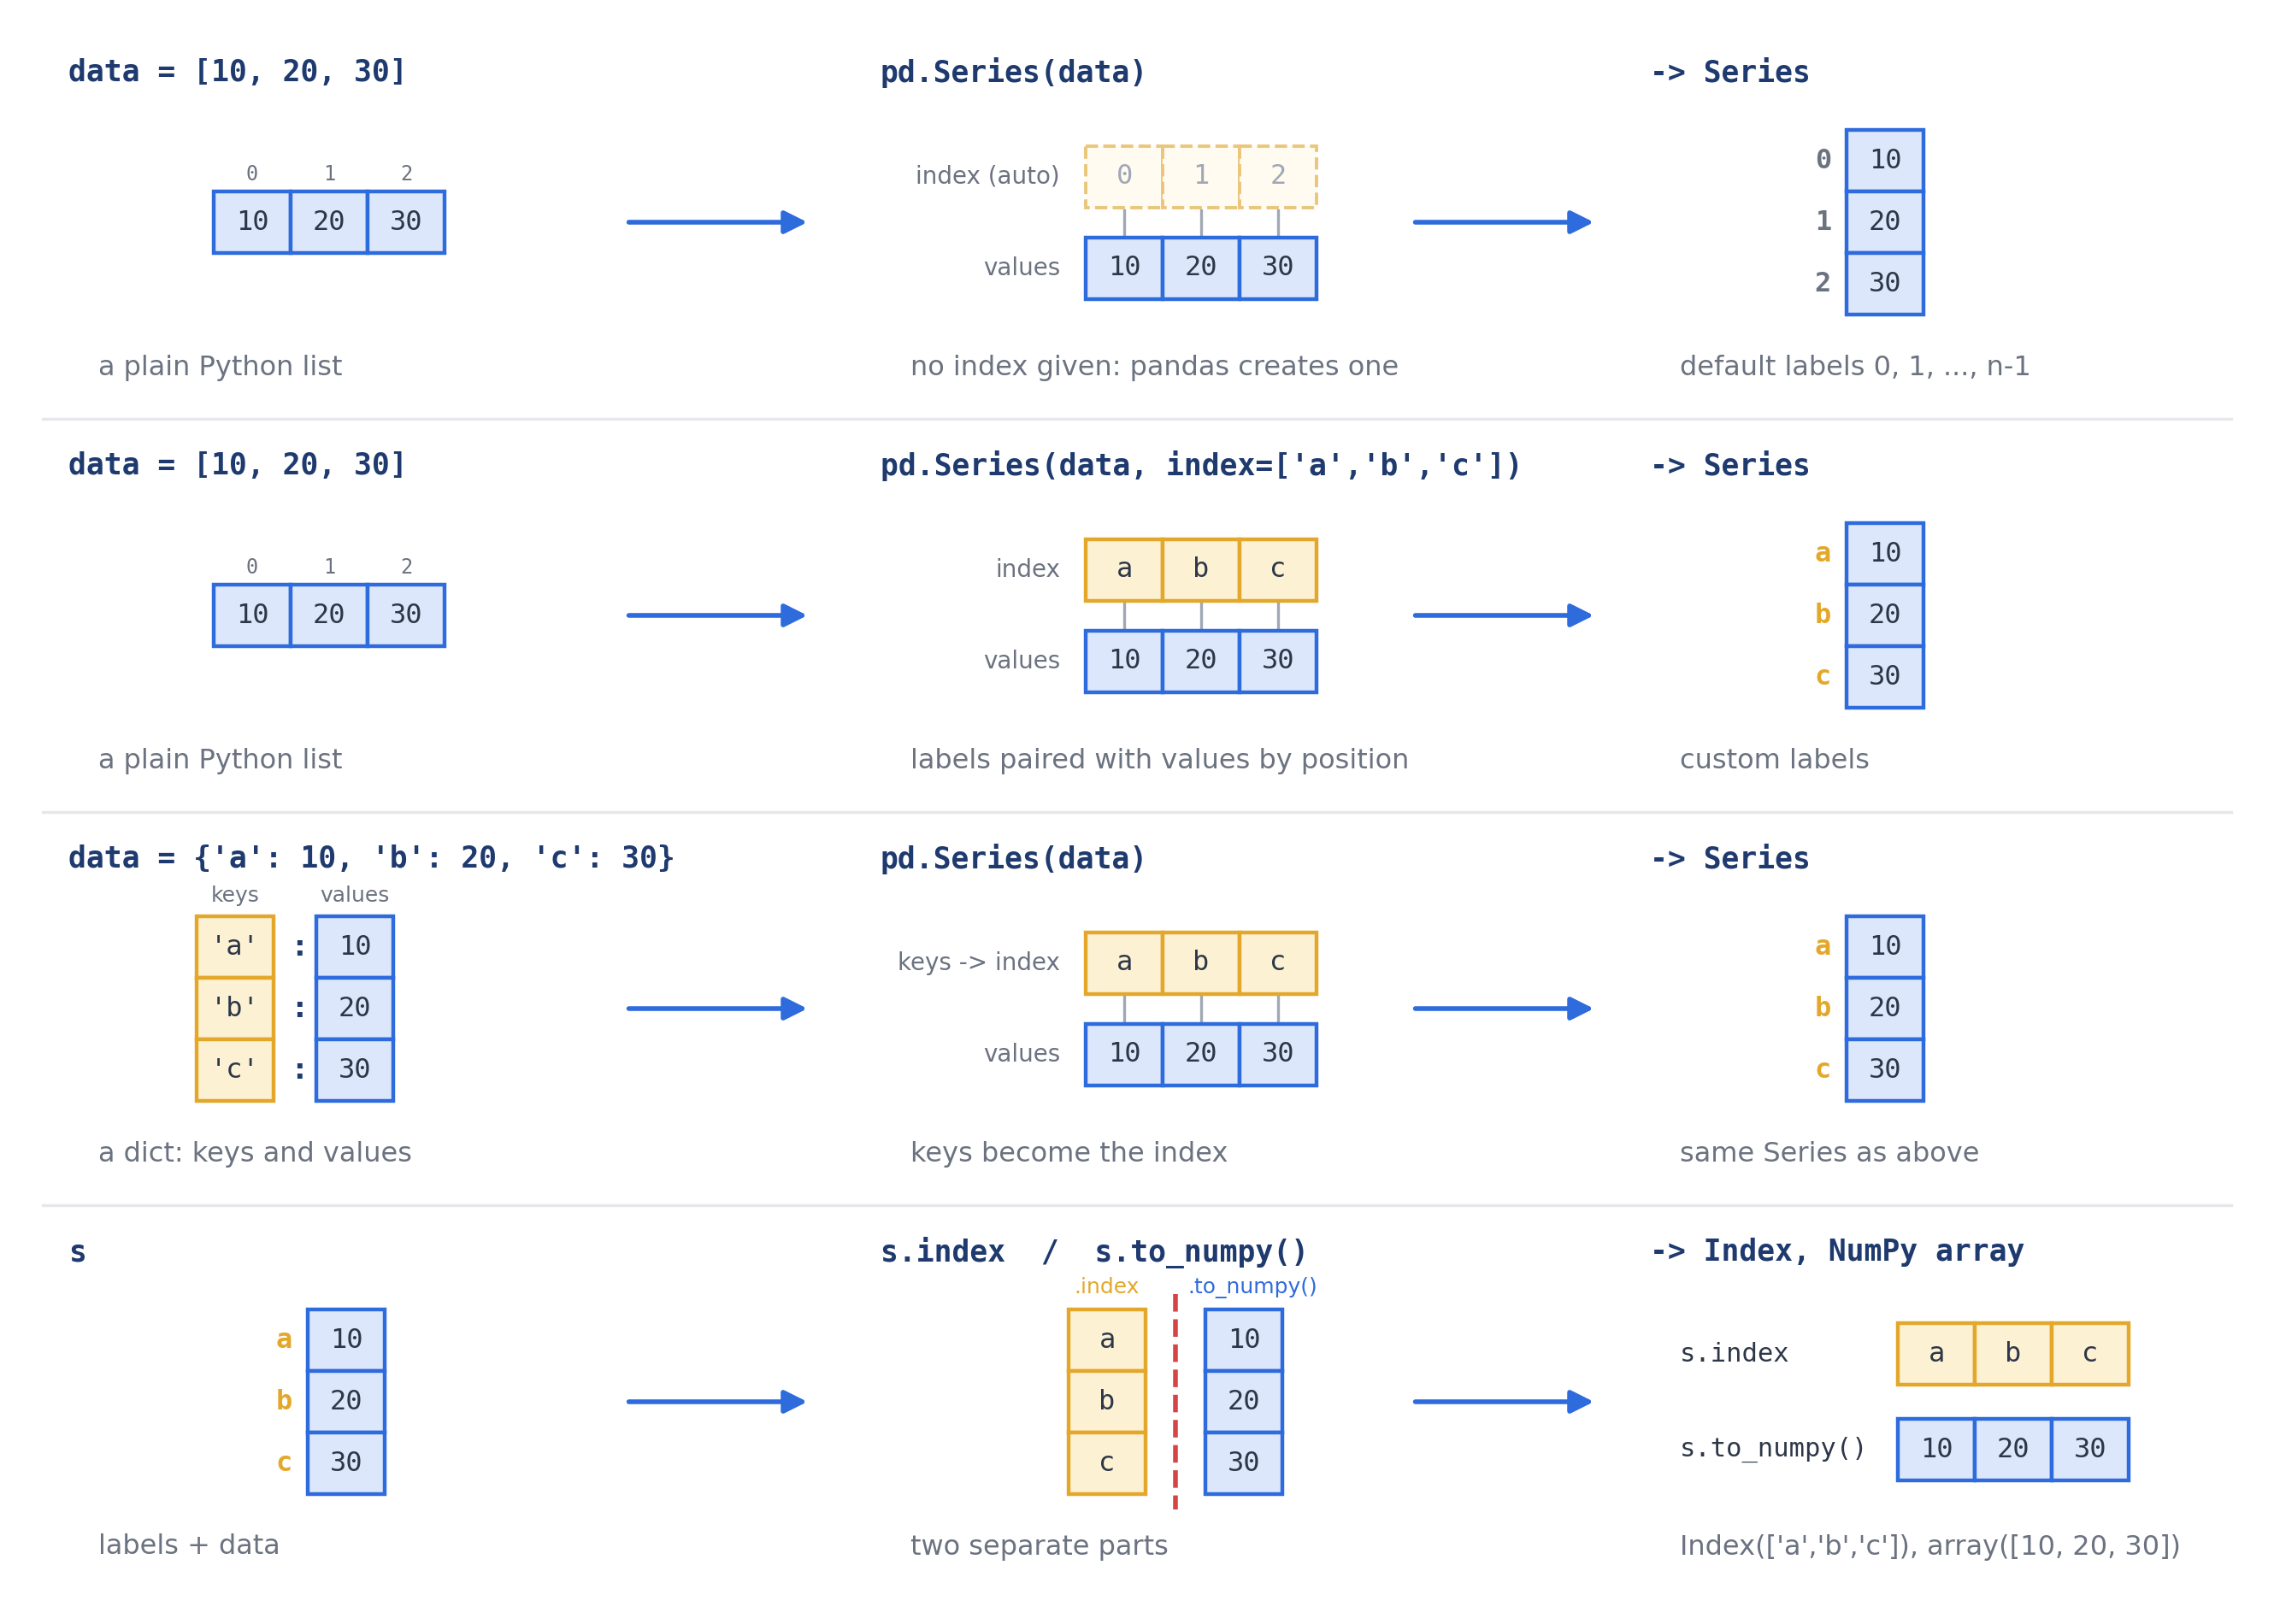
\includegraphics[width=1\textwidth]{contents/images/pandas/sub_series_creation.png}
    \caption{Creating a Series: from a list with the default index $0, \dots, n-1$, from a list with a custom \texttt{index}, and from a dictionary whose keys become the index. The attributes \texttt{.index} and \texttt{.to\_numpy()} return the labels and the data separately.}
\end{figure}

\begin{itemize}
    \item You can create a Series from a list (with or without specifying the \texttt{index} explicitly) or from a dictionary, where the keys automatically become the index.
    \item A Series acts as a NumPy array with labels: you can access the labels via the \texttt{.index} attribute and the raw array via the \texttt{.values} attribute.
\end{itemize}

\lstinputlisting[caption={Creating a Series and accessing its core attributes.}]{contents/listings/pandas/series_creation.py}

\subsection{Accessing Elements: \texttt{loc} vs \texttt{iloc}}
Because an integer can represent both a position and a label, pandas uses two distinct accessors to avoid ambiguity:
\begin{itemize}
    \item \texttt{.loc[label]}: Selects by \textbf{label} (the explicit name in the index). When slicing (\texttt{s.loc['a':'c']}), the stop element is \textbf{included}.
    \item \texttt{.iloc[position]}: Selects by \textbf{position} (0, 1, 2, ..., like standard Python lists). When slicing (\texttt{s.iloc[1:3]}), the stop element is \textbf{excluded}.
\end{itemize}

\begin{figure}[h]
    \centering
    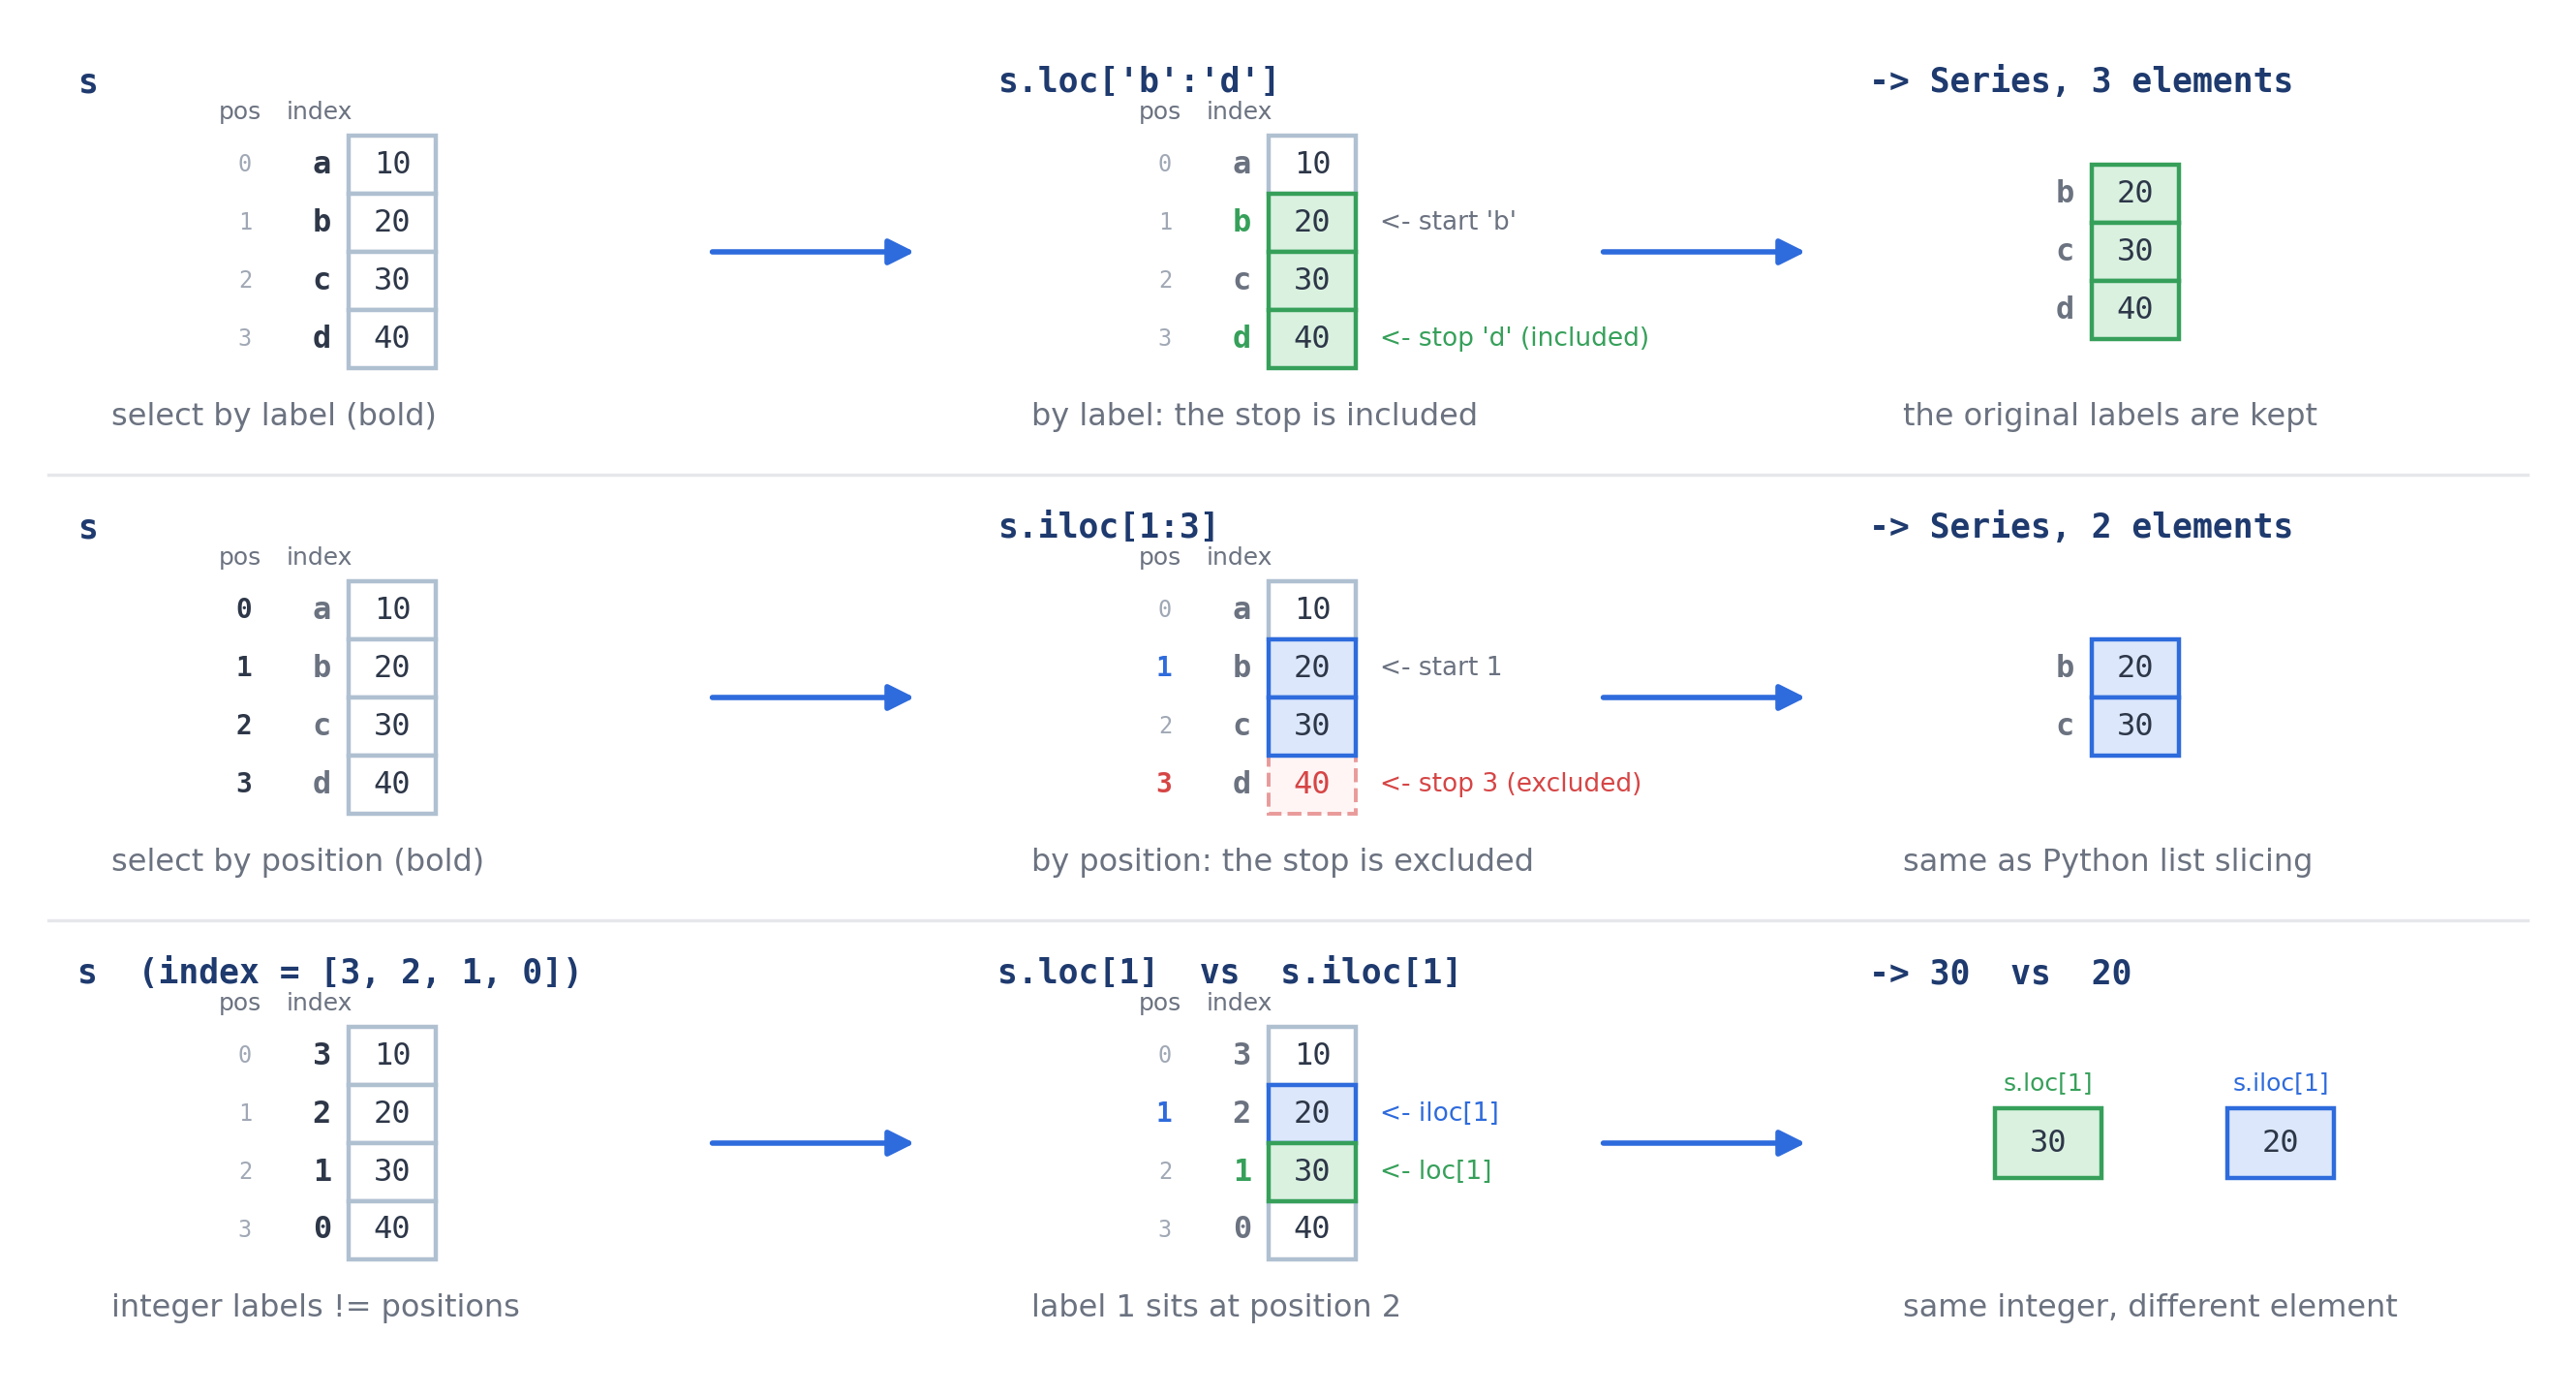
\includegraphics[width=1\textwidth]{contents/images/pandas/sub_loc_iloc.png}
    \caption{\texttt{loc} selects by label and includes the stop of a slice; \texttt{iloc} selects by position and excludes it. With integer labels, \texttt{s.loc[1]} and \texttt{s.iloc[1]} can return different elements.}
\end{figure}

\lstinputlisting[caption={Accessing Series elements using loc and iloc.}]{contents/listings/pandas/series_access.py}

\subsection{Masking and Fancy Indexing}

\begin{itemize}
    \item \textbf{Masking:} Applying a comparison to a Series creates a boolean mask. Because the mask is a Series itself containing labels, it must be used with \texttt{.loc}.
        \begin{figure}[h]
            \centering
            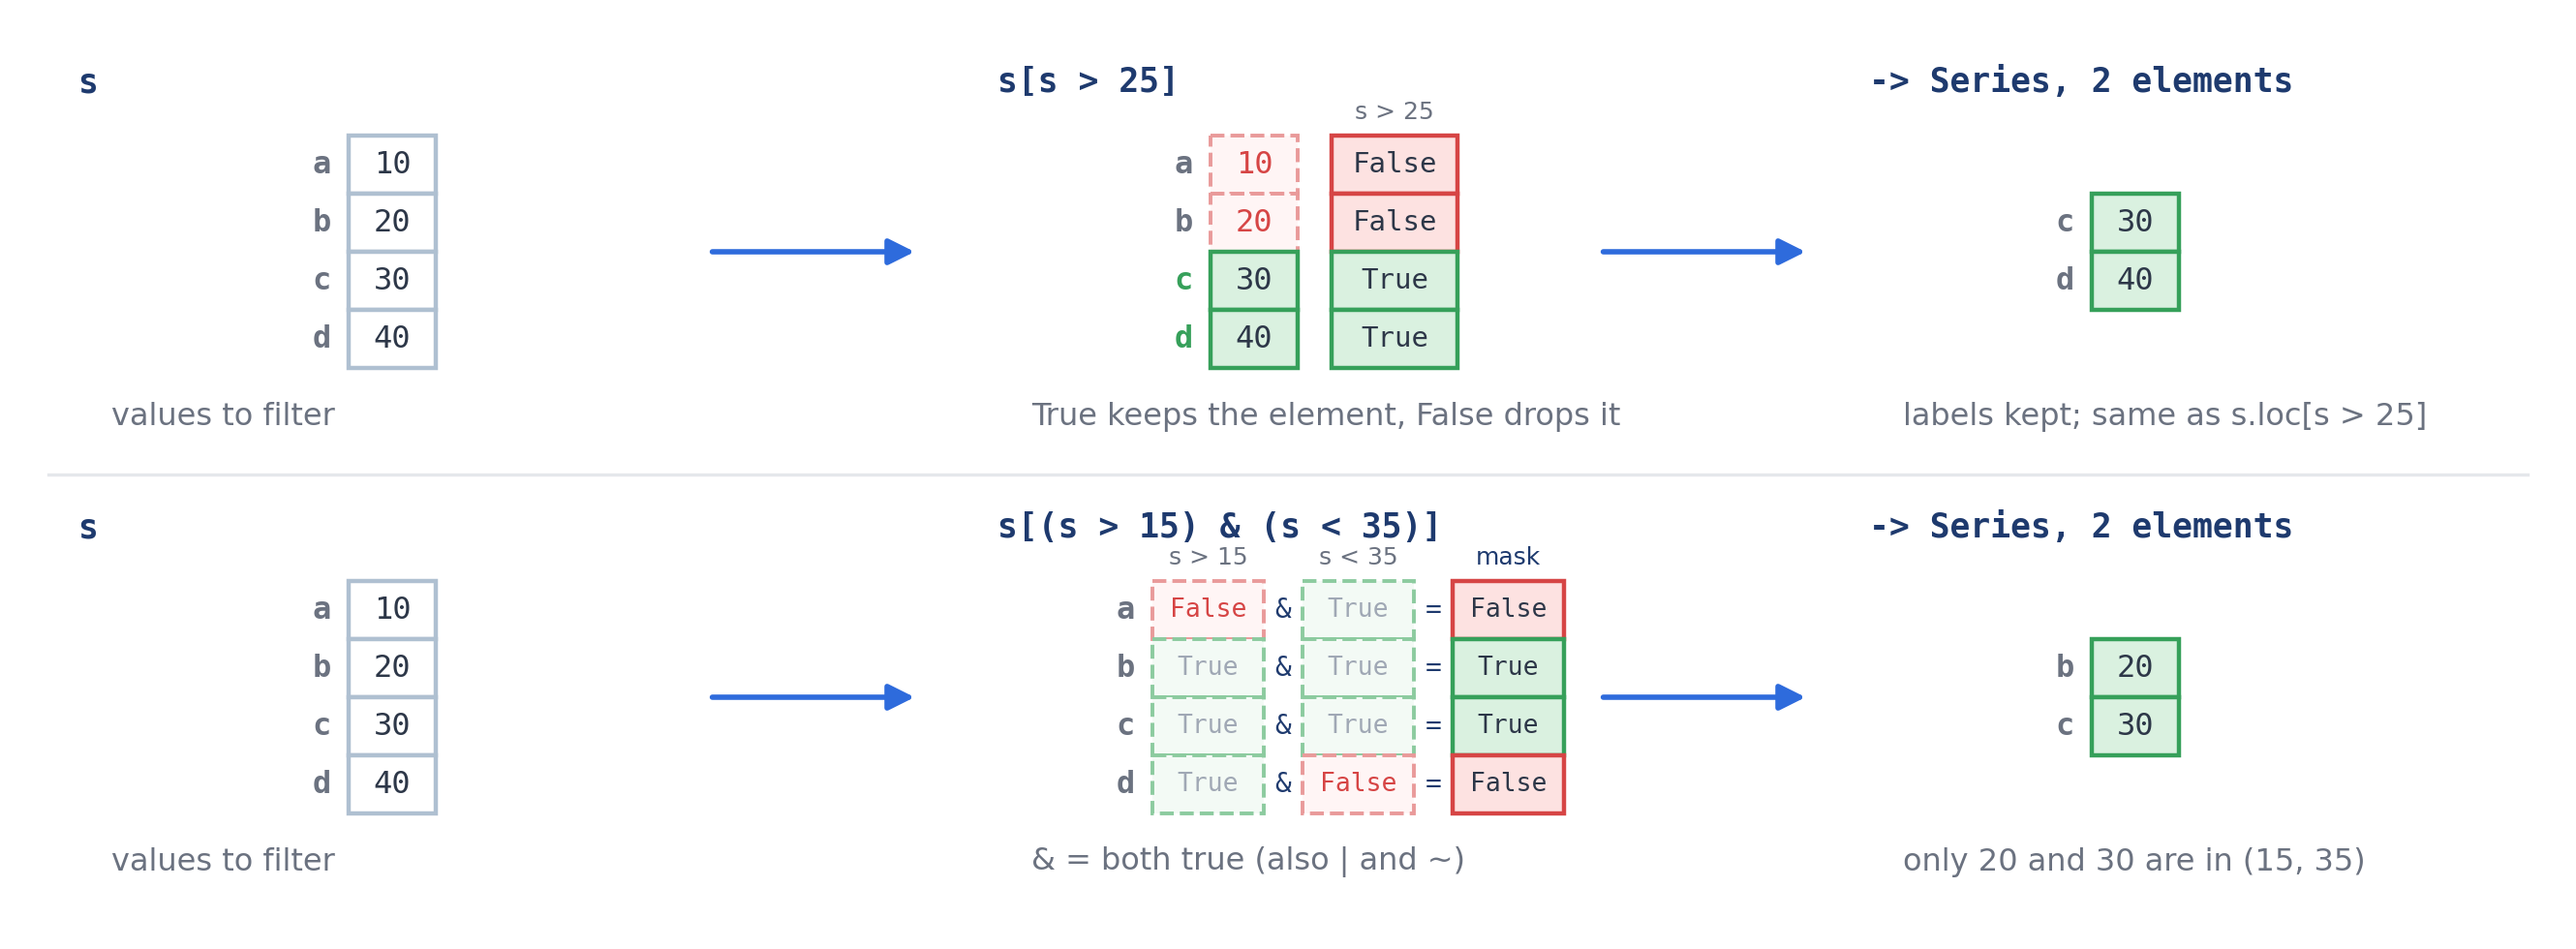
\includegraphics[width=1\textwidth]{contents/images/pandas/sub_masking.png}
            \caption{Boolean masking: a comparison produces a boolean Series with the same index, which keeps only the \texttt{True} elements when passed to \texttt{s[...]} or \texttt{s.loc[...]}. Conditions are combined with \texttt{\&}, \texttt{|}, \texttt{\textasciitilde}; \texttt{.iloc} rejects a boolean Series.}
        \end{figure}
    
    \item \textbf{Fancy Indexing:} You can pass a list of labels to \texttt{.loc} or a list of integer positions to \texttt{.iloc}.
        \begin{figure}[h]
            \centering
            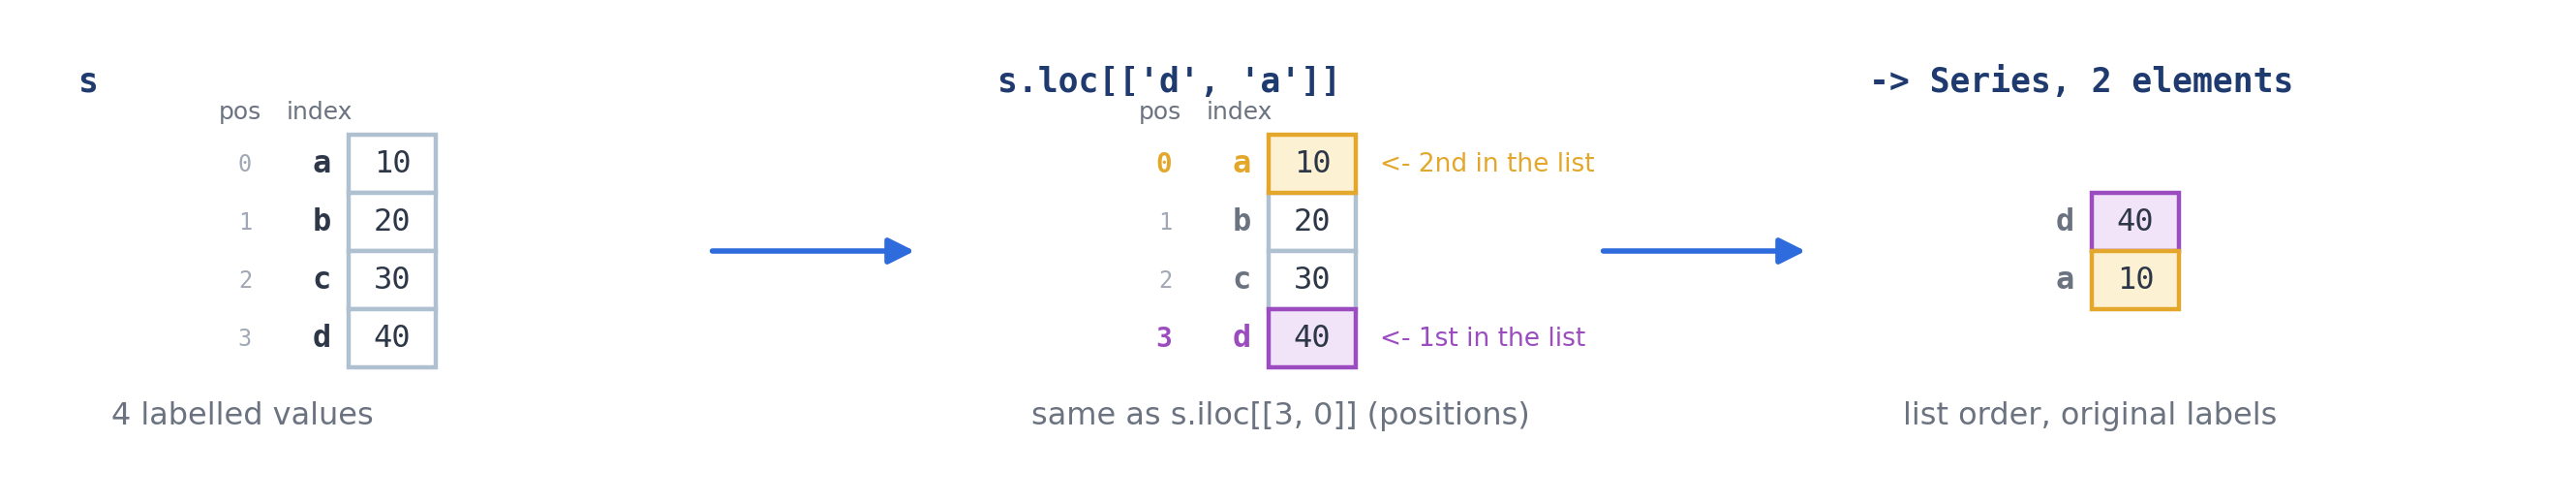
\includegraphics[width=1\textwidth]{contents/images/pandas/sub_fancy_indexing.png}
            \caption{Fancy indexing: a list of labels (\texttt{loc}) or positions (\texttt{iloc}) returns the elements in the order of the list, repetitions included. A label that is not in the index raises a \texttt{KeyError}.}
        \end{figure}

\end{itemize}


\section{DataFrames}

\subsection{A Table of Series}
A DataFrame is a two-dimensional table where each column is an independent Series. While all columns share the same row index, each column maintains its own distinct \texttt{dtype}.

\begin{figure}[h]
    \centering
    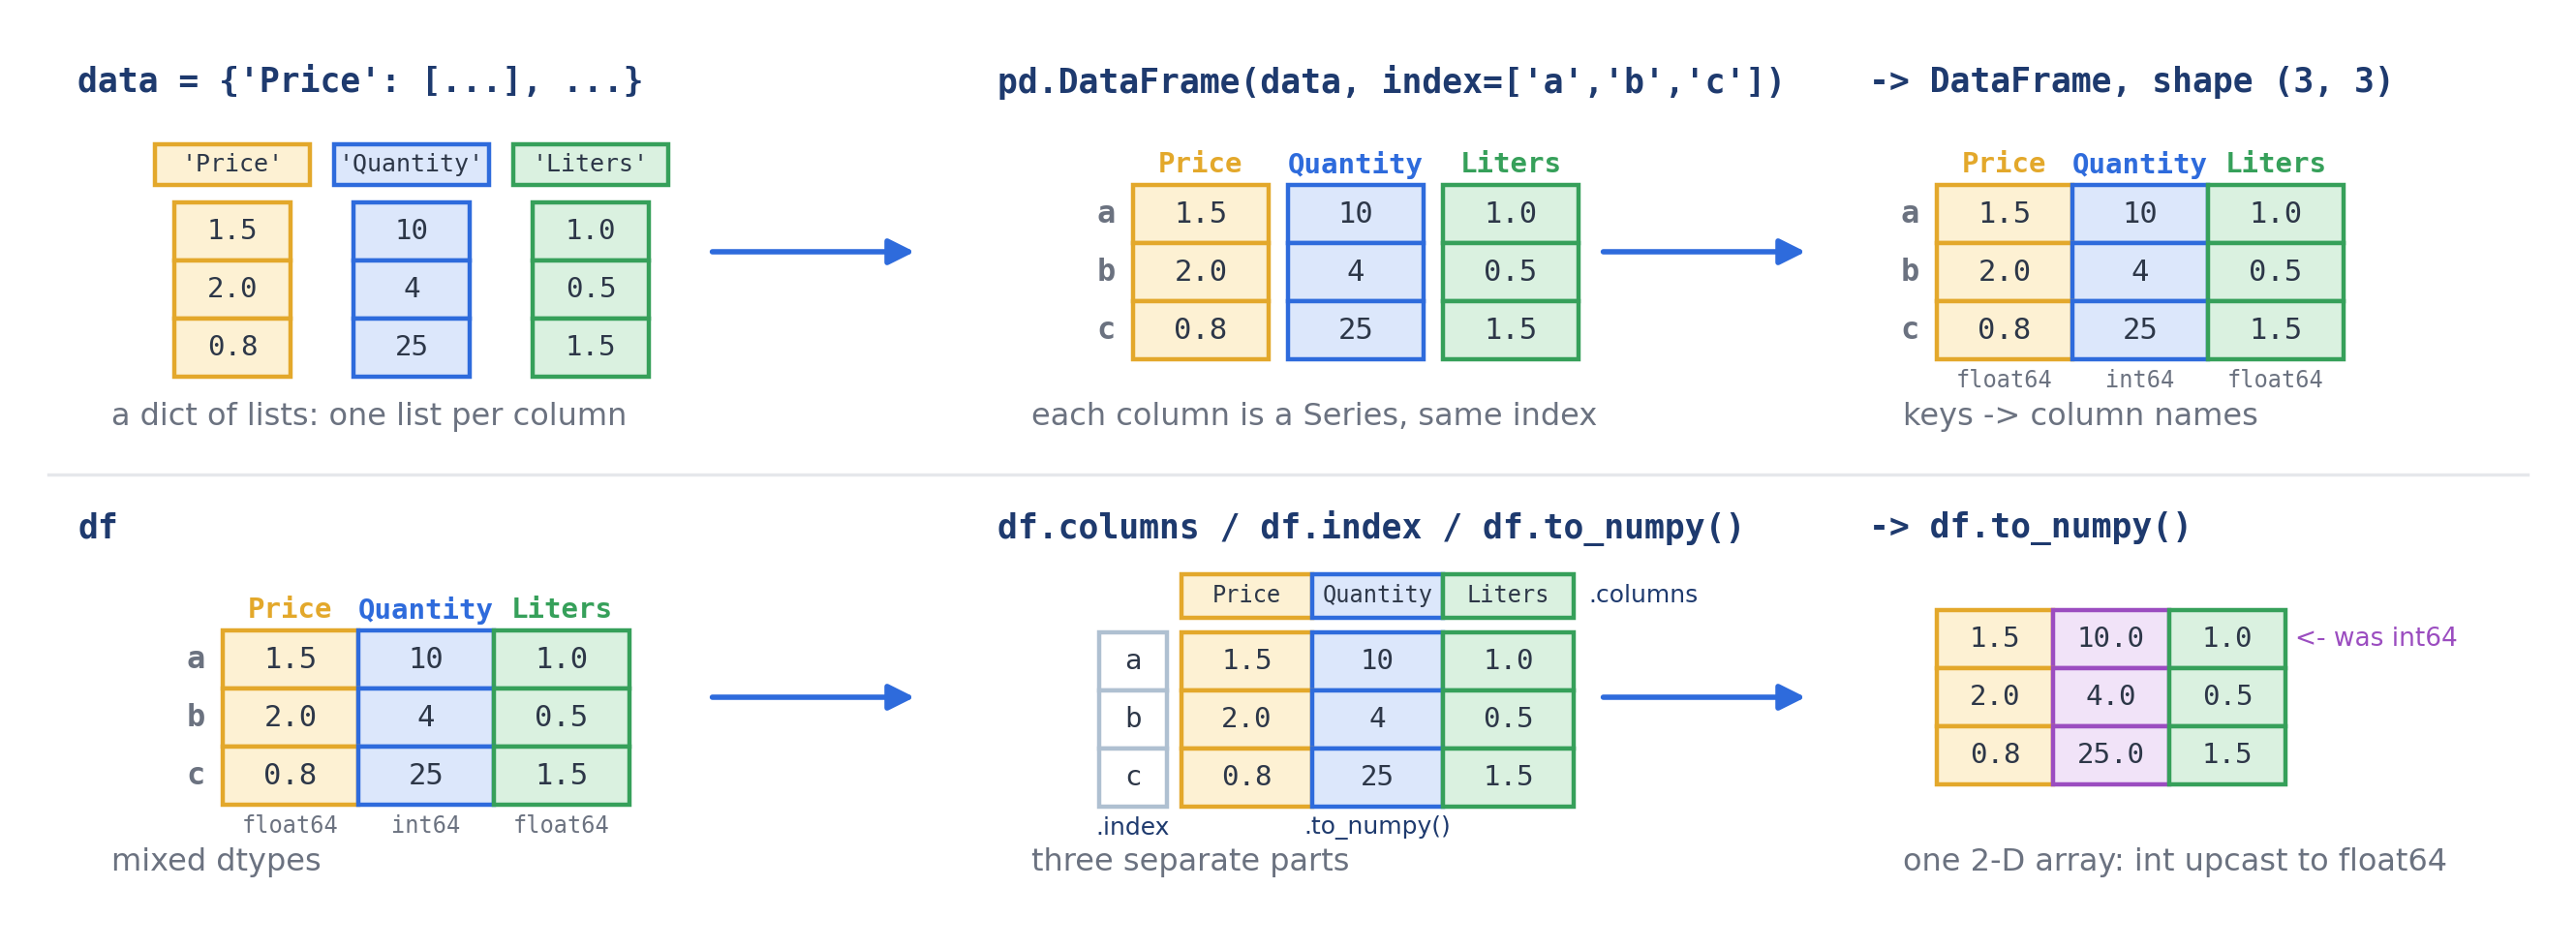
\includegraphics[width=1\textwidth]{contents/images/pandas/sub_dataframe_structure.png}
    \caption{A DataFrame built from a dictionary of lists: each key becomes a column (a Series with its own \texttt{dtype}) and all columns share the same index. \texttt{df.columns}, \texttt{df.index} and \texttt{df.to\_numpy()} return the three parts separately; in the array the \texttt{int64} column is upcast to \texttt{float64}.}
\end{figure}

\begin{itemize}
    \item DataFrames can be created from a dictionary of Series/lists (where keys become column names), a list of dictionaries, or a 2D NumPy array
    \item Core attributes include \texttt{df.columns} (the column names), \texttt{df.index} (the row labels), and \texttt{df.to\_numpy()} (the raw data as a 2D array). When converting to a single NumPy array, pandas upcasts the data to a type capable of holding all columns.
\end{itemize}

\lstinputlisting[caption={Creating and inspecting a DataFrame.}]{contents/listings/pandas/dataframe_creation.py}

\subsection{Accessing Columns and Rows}
On a DataFrame, plain brackets and \texttt{loc}/\texttt{iloc} serve completely different purposes:

\begin{figure}[h]
    \centering
    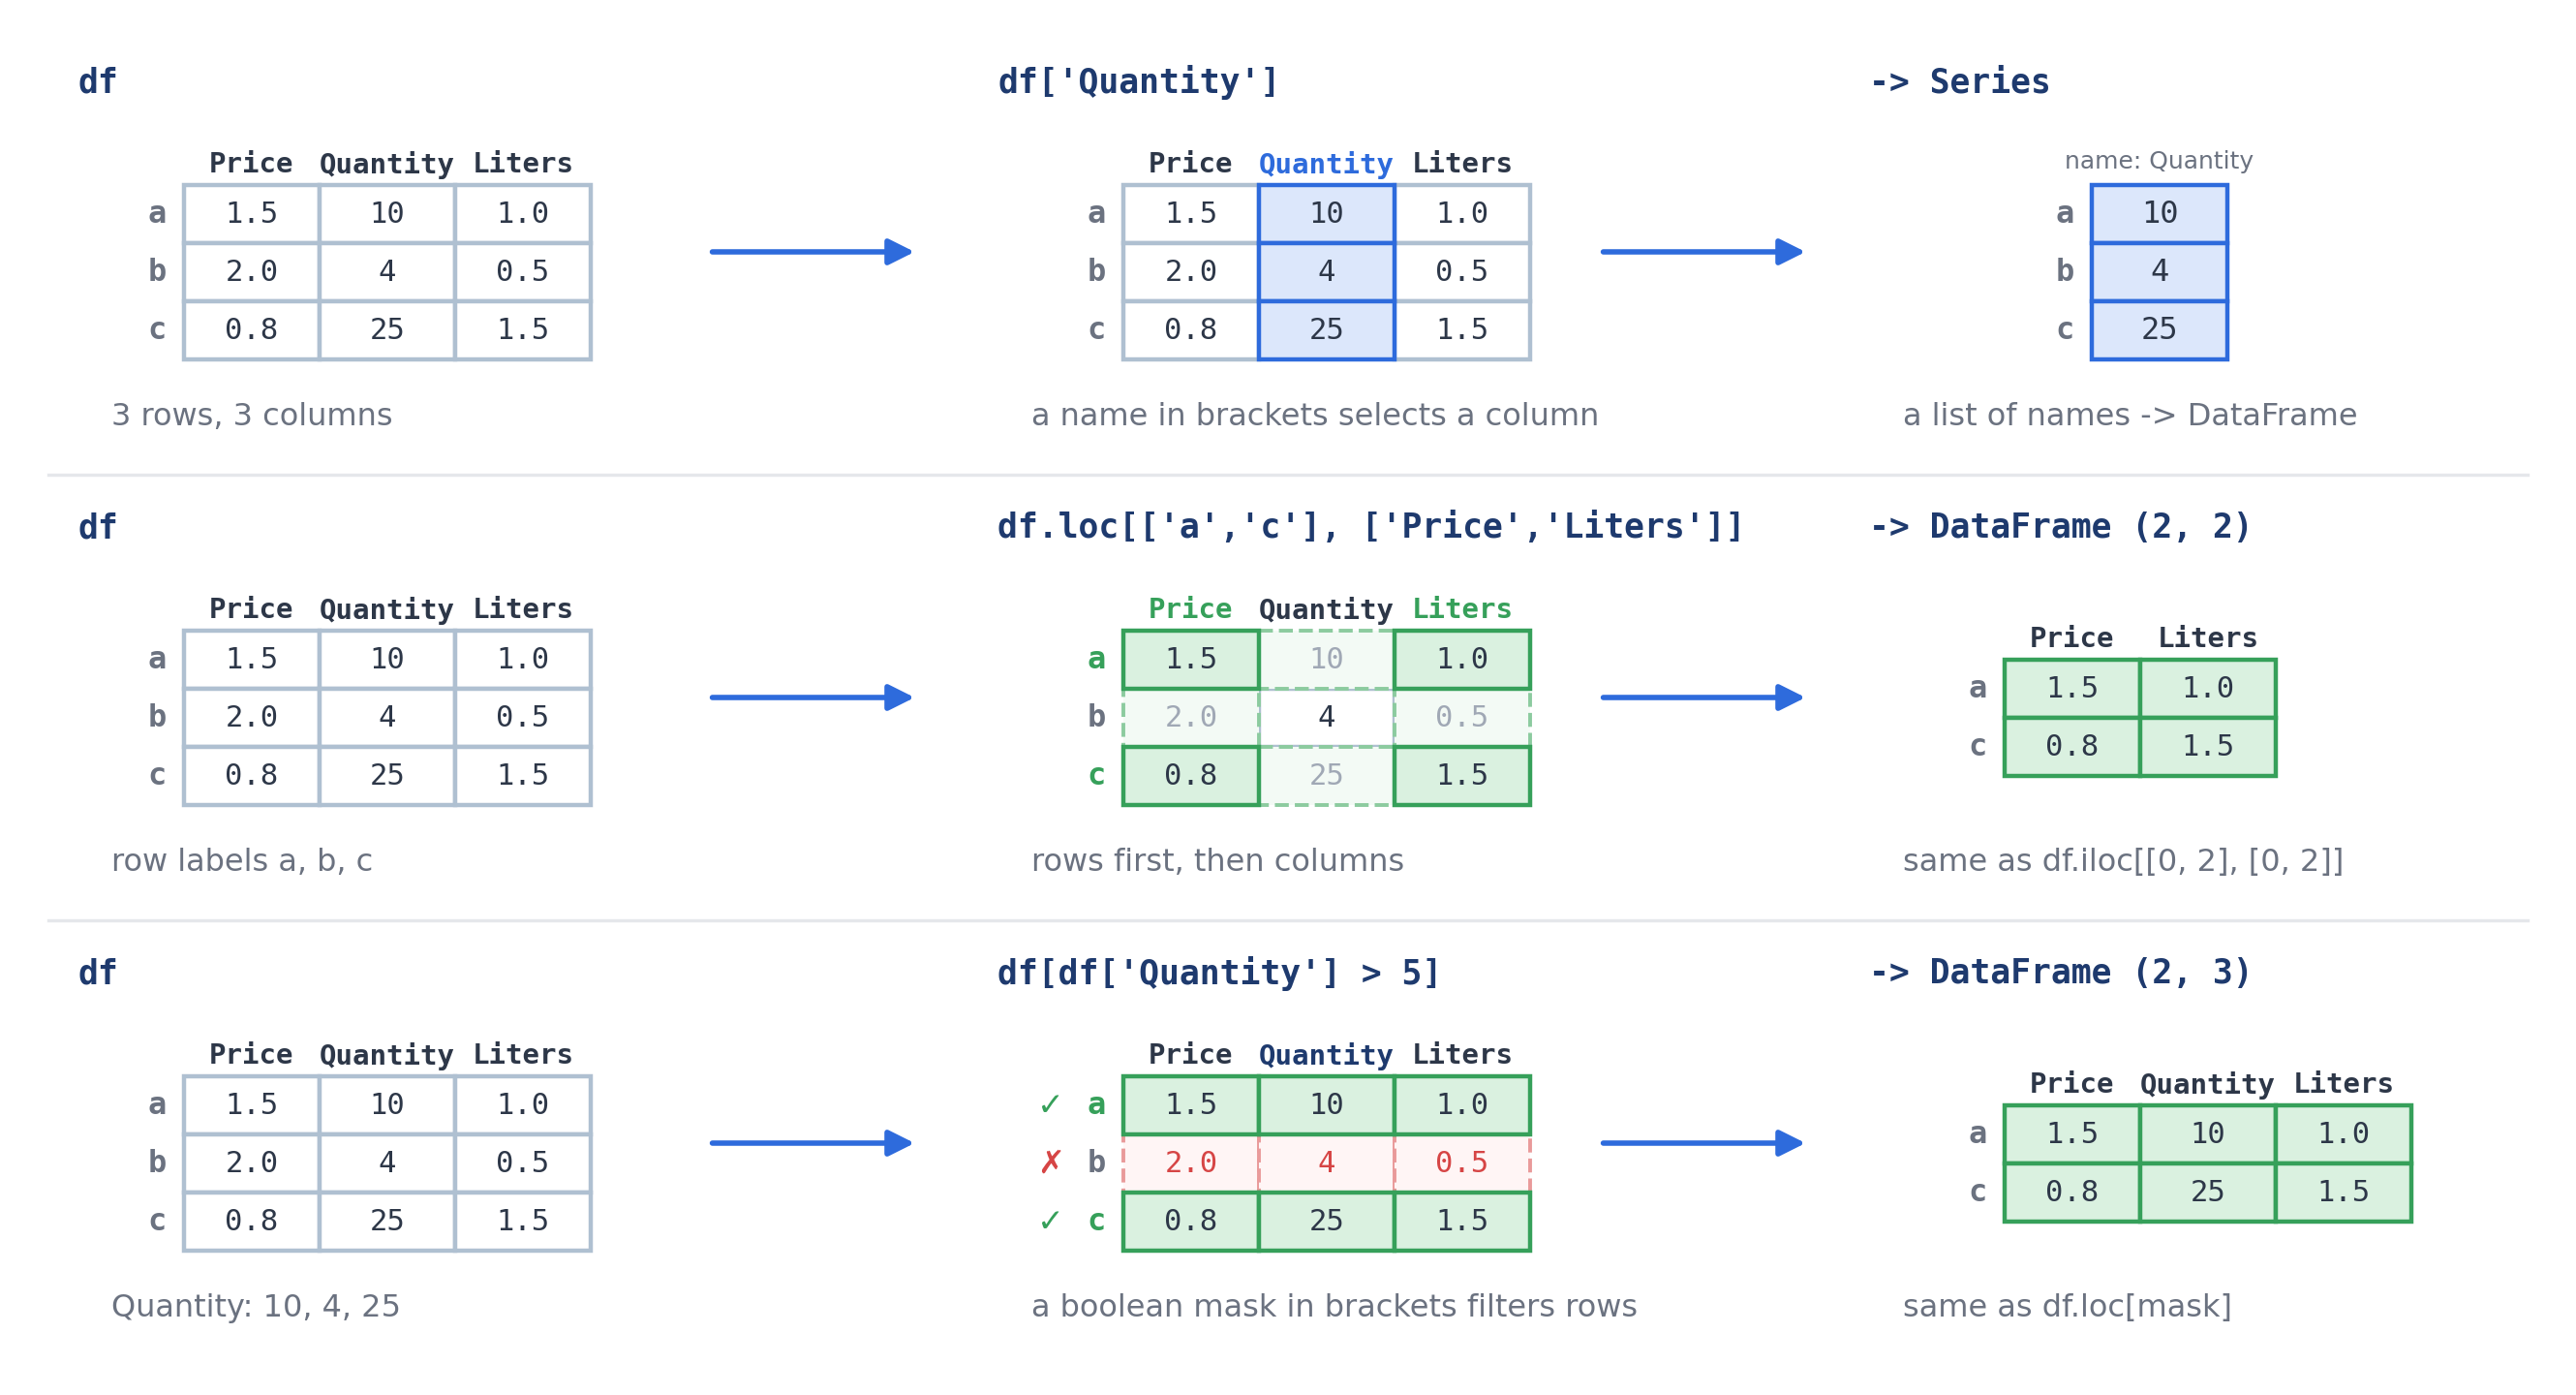
\includegraphics[width=1\textwidth]{contents/images/pandas/sub_dataframe_access.png}
    \caption{Selecting from a DataFrame: a column name in brackets returns a Series, \texttt{df.loc[rows, columns]} returns the intersection of the chosen rows and columns, and a boolean mask in brackets keeps only the rows where it is \texttt{True}.}
\end{figure}

\begin{itemize}
    \item \textbf{Columns:} A name (or list of names) in plain brackets selects columns (\texttt{df['Quantity']} returns a Series, \texttt{df[['Price', 'Liters']]} returns a DataFrame).
    \item \textbf{Rows \& Grids:} \texttt{.loc} and \texttt{.iloc} select rows, or both rows and columns if two selectors are provided (\texttt{df.loc[rows, columns]}).
    \item \textbf{Masking shortcut:} A boolean mask passed directly in plain brackets (e.g., \texttt{df[mask]}) is a ubiquitous shorthand for filtering rows, equivalent to \texttt{df.loc[mask]}.
\end{itemize}

\lstinputlisting[caption={Selecting rows, columns, and applying boolean masks on a DataFrame.}]{contents/listings/pandas/dataframe_access.py}

\subsection{Adding, Modifying, and Copy-on-Write}
You can add or replace columns by assigning them to a name (\texttt{df["NewCol"] = ...}). Methods like \texttt{rename} and \texttt{drop} return a new DataFrame without altering the original.

\begin{figure}[h]
    \centering
    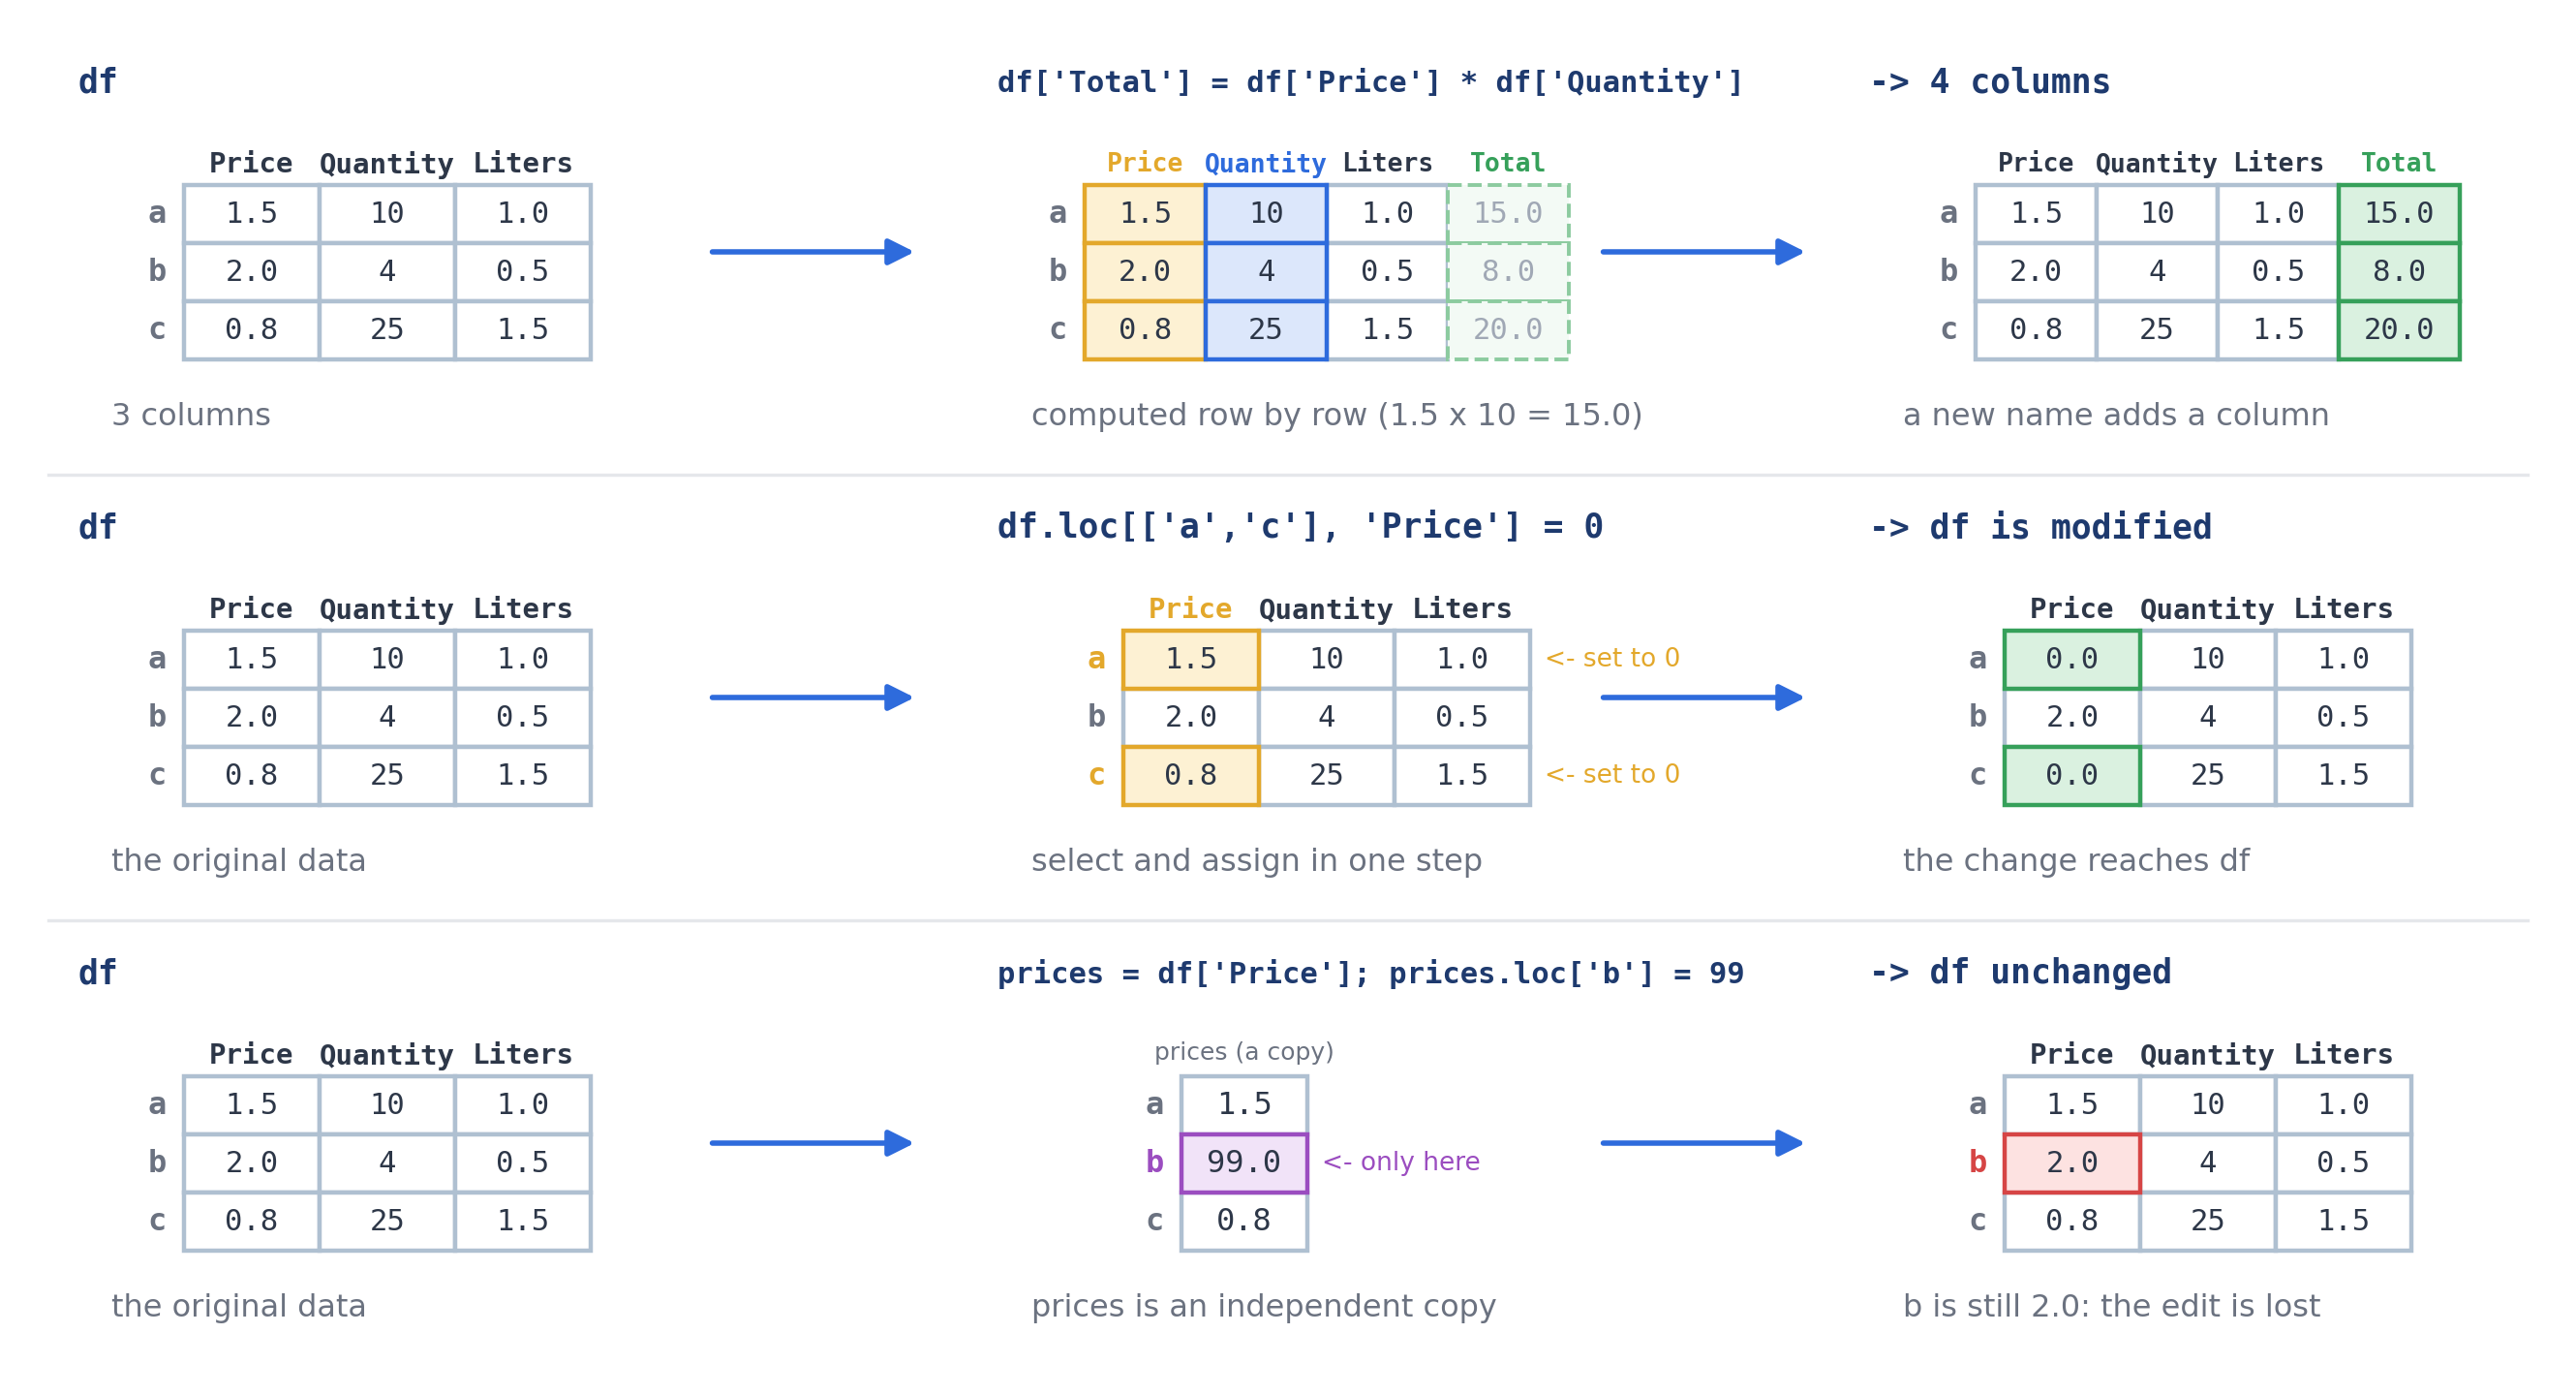
\includegraphics[width=1\textwidth]{contents/images/pandas/sub_dataframe_modify.png}
    \caption{Modifying a DataFrame: assigning to a new name adds a column; \texttt{df.loc[rows, column] = value} changes \texttt{df} in a single step; with Copy-on-Write, an edit made through an intermediate variable changes only the copy and is lost for \texttt{df}.}
\end{figure}

\textbf{Copy-on-Write (pandas 3.0+):}
Any piece of data extracted from a DataFrame (a column, slice, or mask) behaves as an independent copy. To safely modify the original DataFrame, you must perform the selection and assignment in a single operation:
\begin{itemize}
    \item \textbf{Correct:} \texttt{df.loc[["a", "c"], "Price"] = 0} (modifies \texttt{df} directly).
    \item \textbf{Incorrect:} \texttt{prices = df["Price"]; prices.loc["b"] = 99} (modifies the copy, leaving \texttt{df} unchanged).
\end{itemize}

\lstinputlisting[caption={Adding columns and assigning values properly.}]{contents/listings/pandas/dataframe_modify.py}



\section{Computation with pandas}
Pandas supports three main types of computational operations: unary operations, aggregations, and operations between pandas objects.

\subsection{Unary Operations}
Unary operations are applied element-by-element. You can perform standard arithmetic (e.g., \texttt{s / 4 + 1}) or apply NumPy universal functions (e.g., \texttt{np.abs(s)}) directly to a Series or DataFrame. The resulting object retains the exact same index and labels as the original.

\begin{figure}[h]
    \centering
    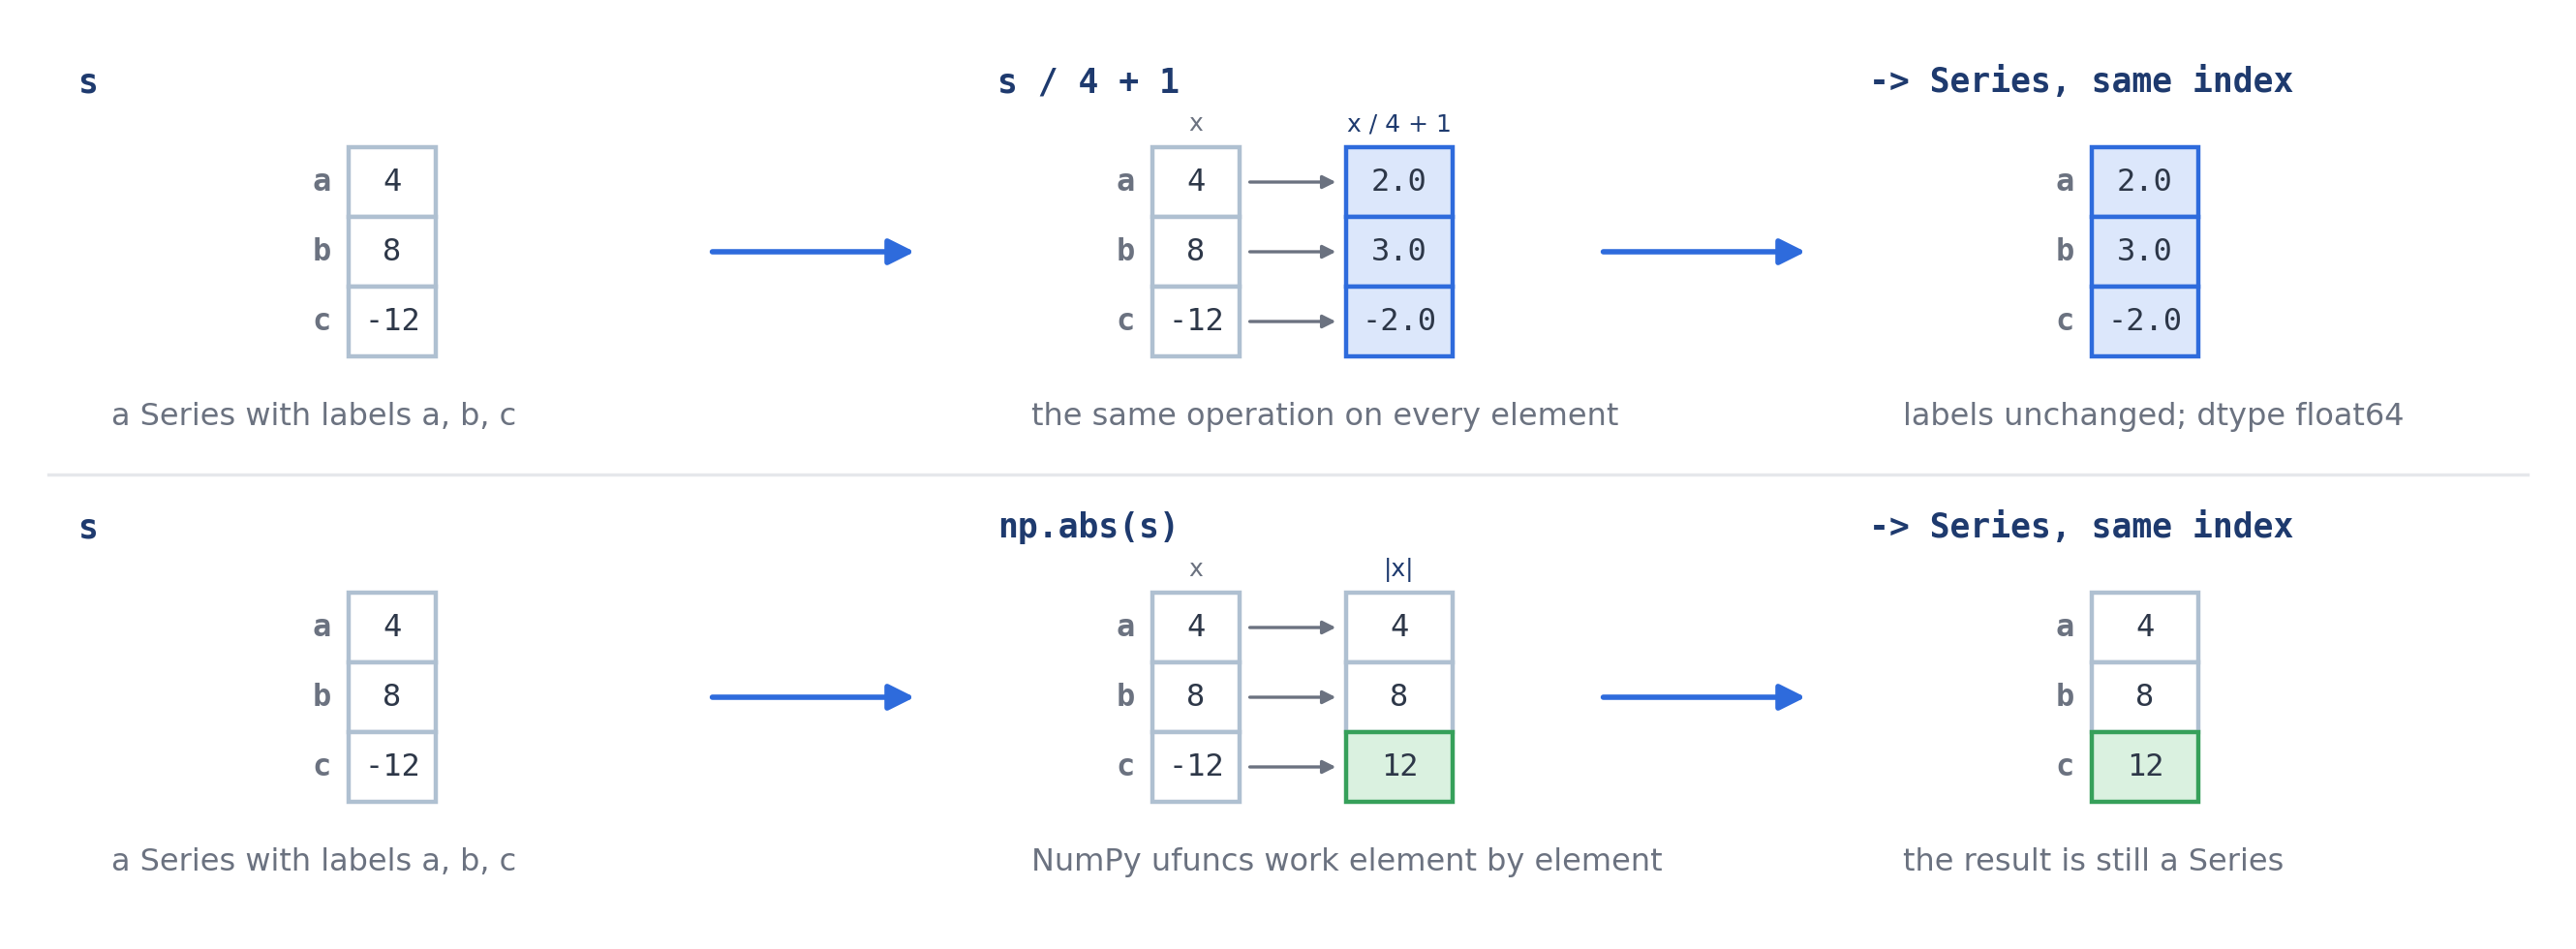
\includegraphics[width=1\textwidth]{contents/images/pandas/sub_unary.png}
    \caption{Unary operations: arithmetic expressions such as \texttt{s / 4 + 1} and NumPy ufuncs such as \texttt{np.abs(s)} are applied to every element, and the result keeps the original index.}
\end{figure}

\lstinputlisting[caption={Applying arithmetic and NumPy ufuncs to a Series.}]{contents/listings/pandas/pandas_unary.py}

\subsection{Operations Between Objects: Alignment}
When performing binary operations (like \texttt{+}, \texttt{-}, \texttt{*}, \texttt{/}) between Series or DataFrames, pandas pairs the elements \textbf{by label, not by position}.

\begin{figure}[h]
    \centering
    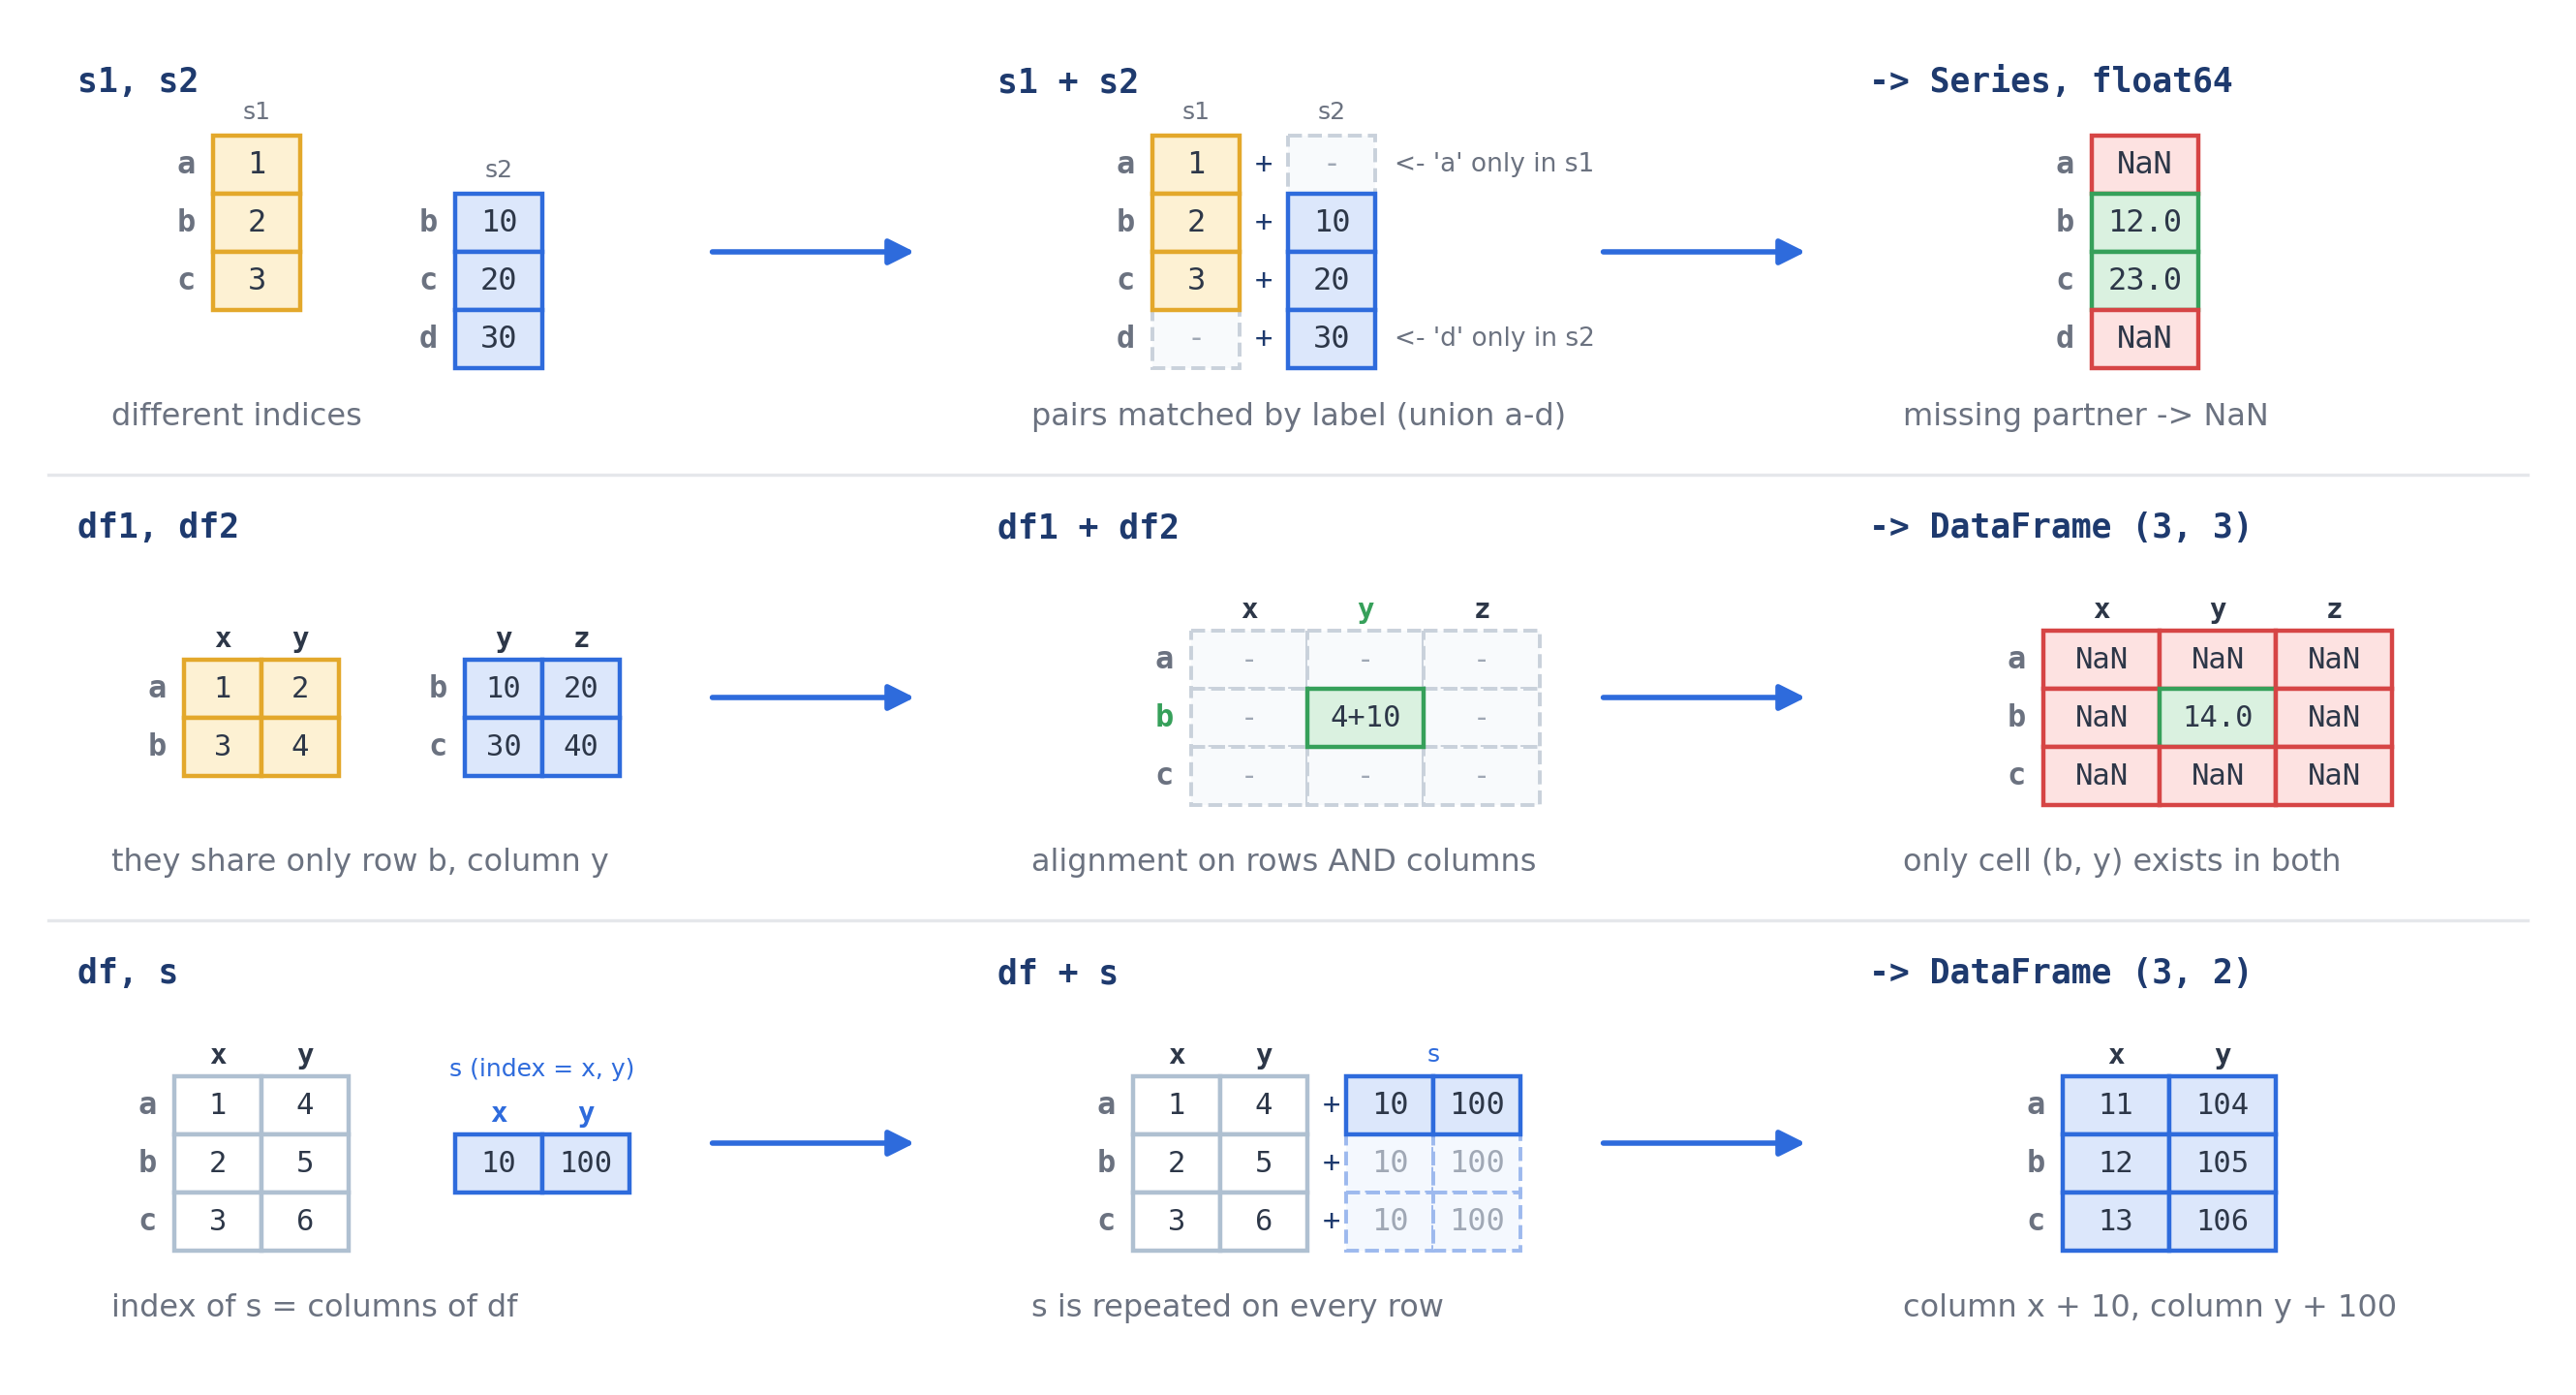
\includegraphics[width=1\textwidth]{contents/images/pandas/sub_alignment.png}
    \caption{Label alignment: two Series are matched by label over the union of their indices, and a label missing on one side gives \texttt{NaN}. Two DataFrames are aligned on both rows and columns. A Series added to a DataFrame is matched to its columns and broadcast over every row.}
\end{figure}

\begin{itemize}
    \item \textbf{Series + Series:} pandas aligns the two Series based on their indices. If a label exists in one Series but not the other, the result for that label is \texttt{NaN} (Not a Number). The final index is the sorted union of both indices. Because \texttt{NaN} is a floating-point value, introducing it will upcast an integer array to \texttt{float64}.
    \item \textbf{DataFrame + DataFrame:} Alignment happens on both axes (rows and columns). A cell only computes a valid result if both its row label and column label exist in both DataFrames; otherwise, it becomes \texttt{NaN}.
    \item \textbf{Broadcasting (DataFrame + Series):} When operating between a DataFrame and a Series, pandas matches the index of the Series to the \textbf{columns} of the DataFrame. The Series is then broadcast (repeated) across every row of the DataFrame. 
\end{itemize}

\lstinputlisting[caption={Automatic label alignment and broadcasting.}]{contents/listings/pandas/pandas_alignment.py}

\subsection{Aggregations and Normalization}
Aggregation functions (such as \texttt{mean}, \texttt{std}, \texttt{min}, \texttt{max}, \texttt{sum}) reduce the data.

\begin{figure}[h]
    \centering
    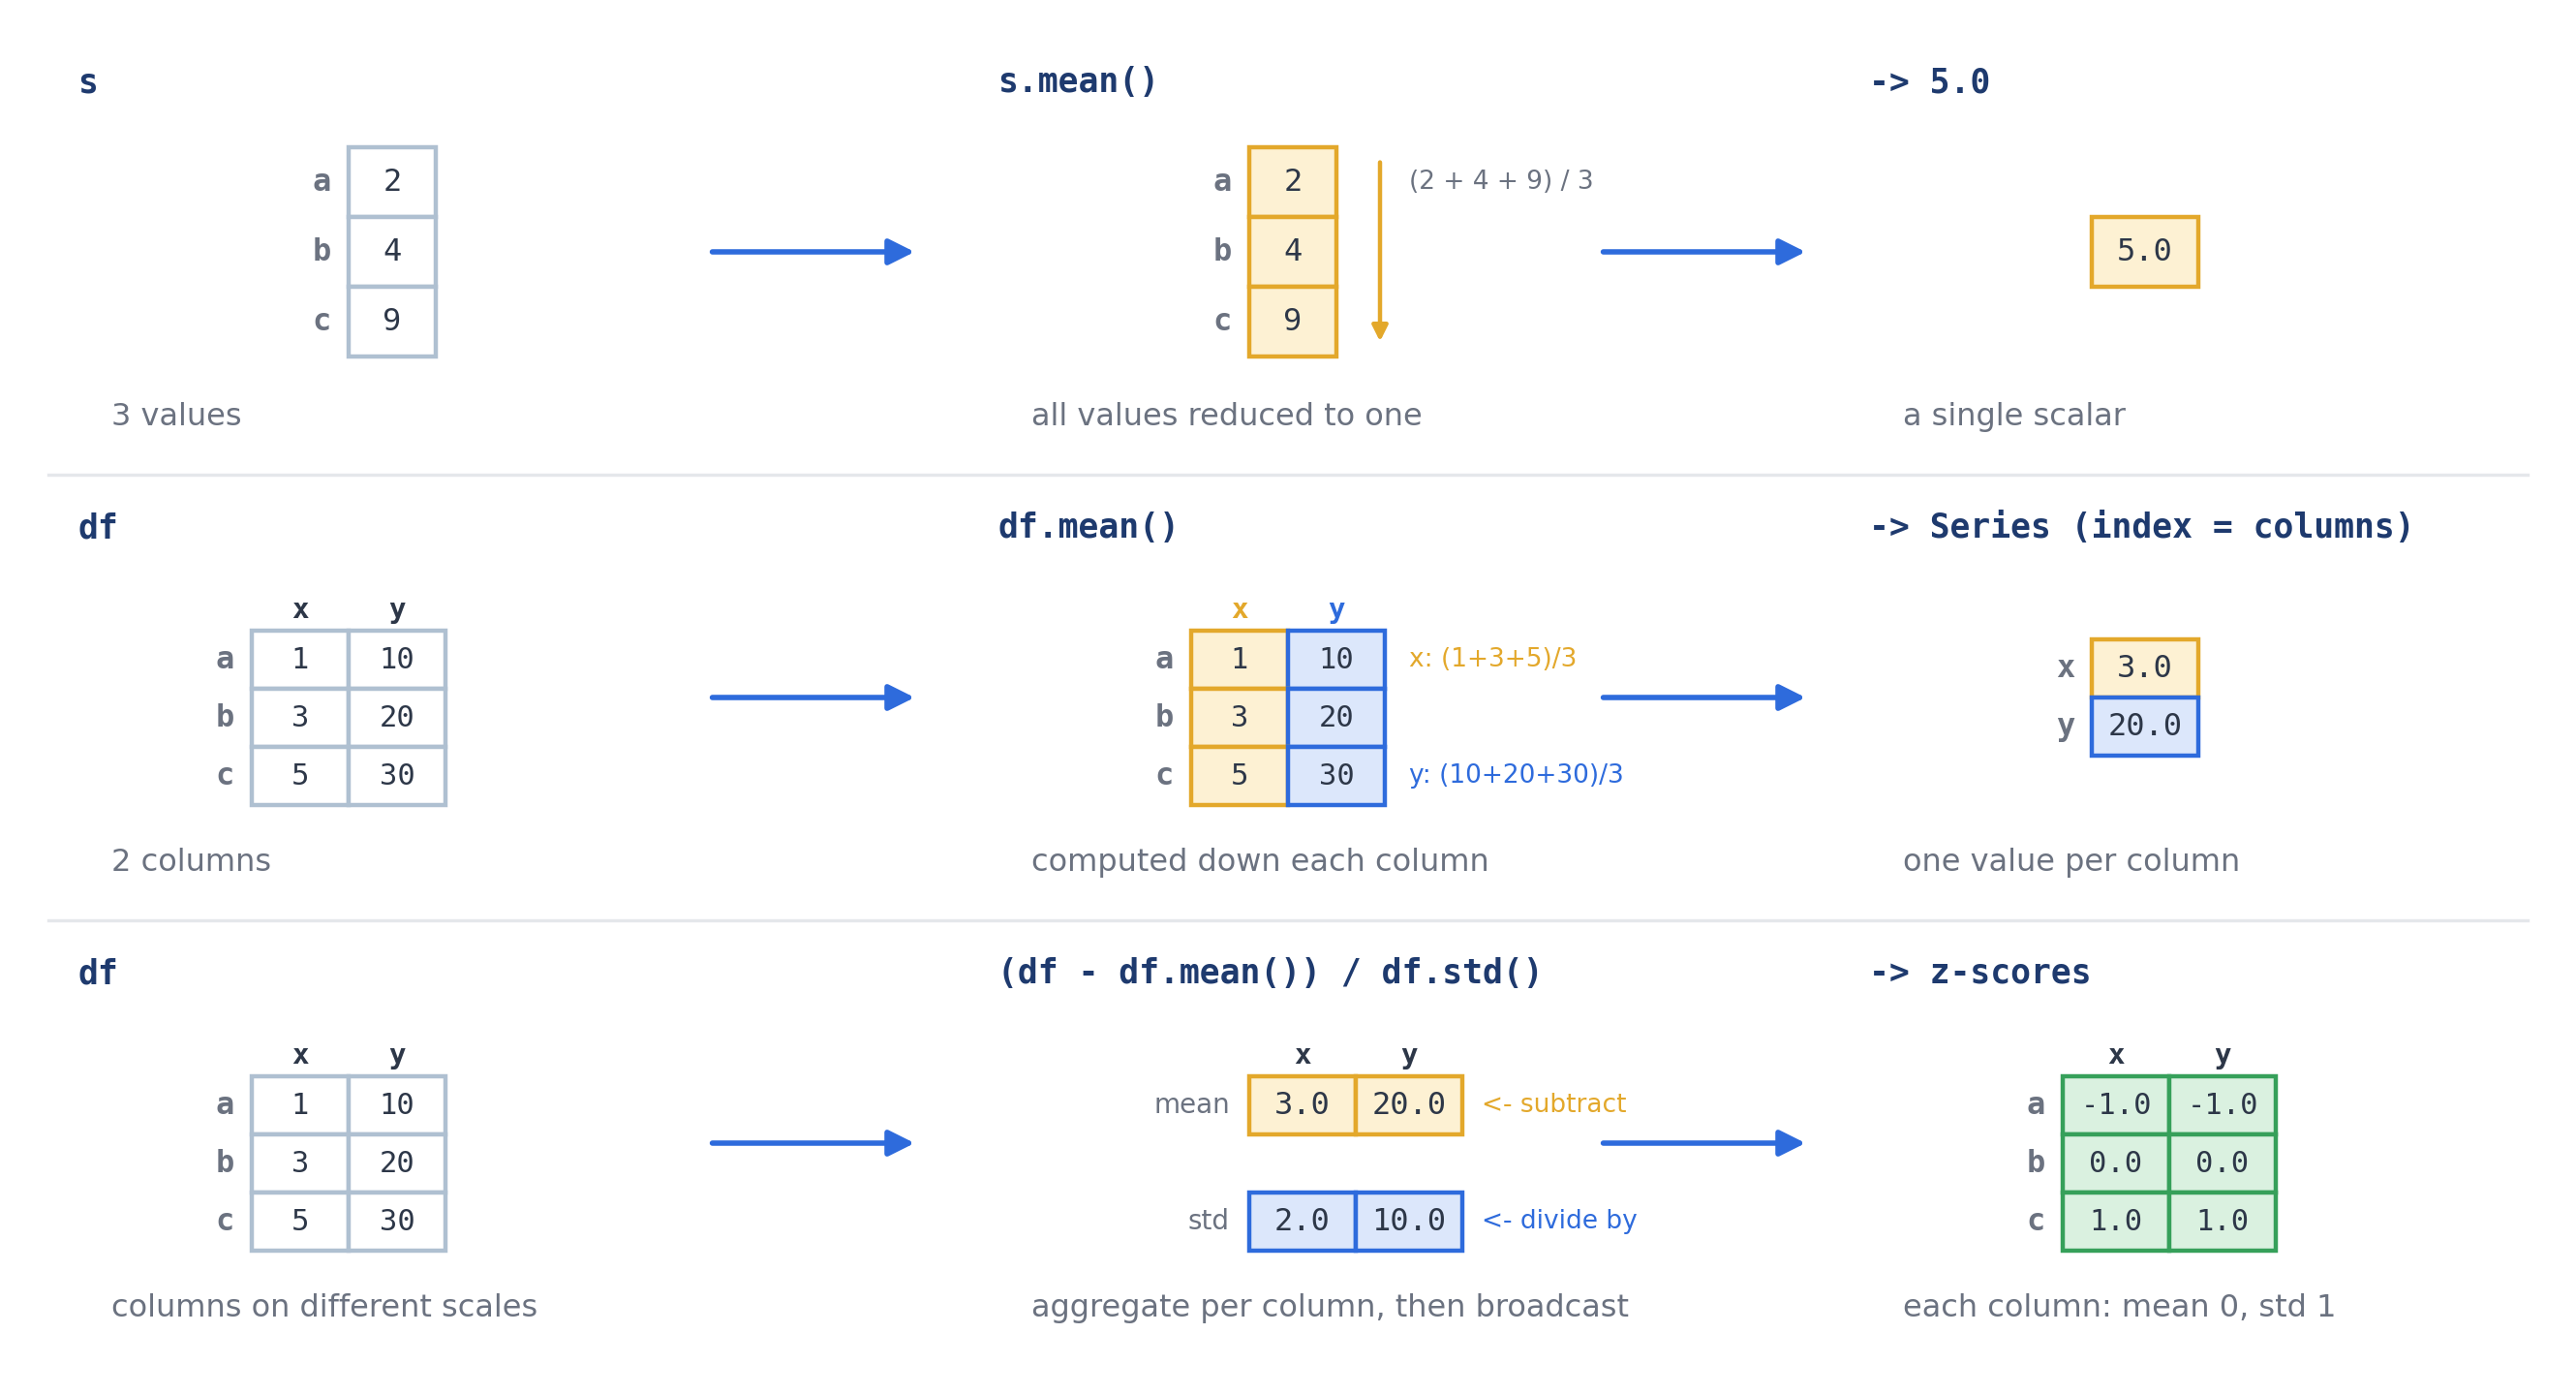
\includegraphics[width=1\textwidth]{contents/images/pandas/sub_aggregations.png}
    \caption{Aggregations: on a Series \texttt{mean()} returns a scalar, on a DataFrame it returns a Series with one value per column. Z-score normalization combines column-wise aggregation and broadcasting: each column ends up with mean 0 and standard deviation 1 (sample \texttt{std}, $\mathrm{ddof}=1$).}
\end{figure}

\begin{itemize}
    \item On a \textbf{Series}, an aggregation returns a single scalar value.
    \item On a \textbf{DataFrame}, the aggregation is computed column by column (iterating over the rows), returning a Series with one value per column.
    \item \textbf{Standard Deviation Note:} By default, \texttt{df.std()} calculates the sample standard deviation (dividing by $n-1$), which differs from NumPy's \texttt{np.std()} (which divides by $n$). To match NumPy's behavior, use \texttt{df.std(ddof=0)}.
\end{itemize}

A common data preprocessing task is Z-score normalization, which leverages both column-wise aggregation and broadcasting to execute without a single loop[cite: 142].

\lstinputlisting[caption={Aggregating DataFrames and Z-score normalization.}]{contents/listings/pandas/pandas_aggregations.py}



\section{Combining Series and DataFrames}
pandas provides two primary functions for putting DataFrames and Series together: \texttt{pd.concat} for stacking them, and \texttt{pd.merge} for joining them based on common values.

\subsection{Concatenation}
The \texttt{pd.concat} function stacks objects (vertically by default). 

\begin{figure}[h]
    \centering
    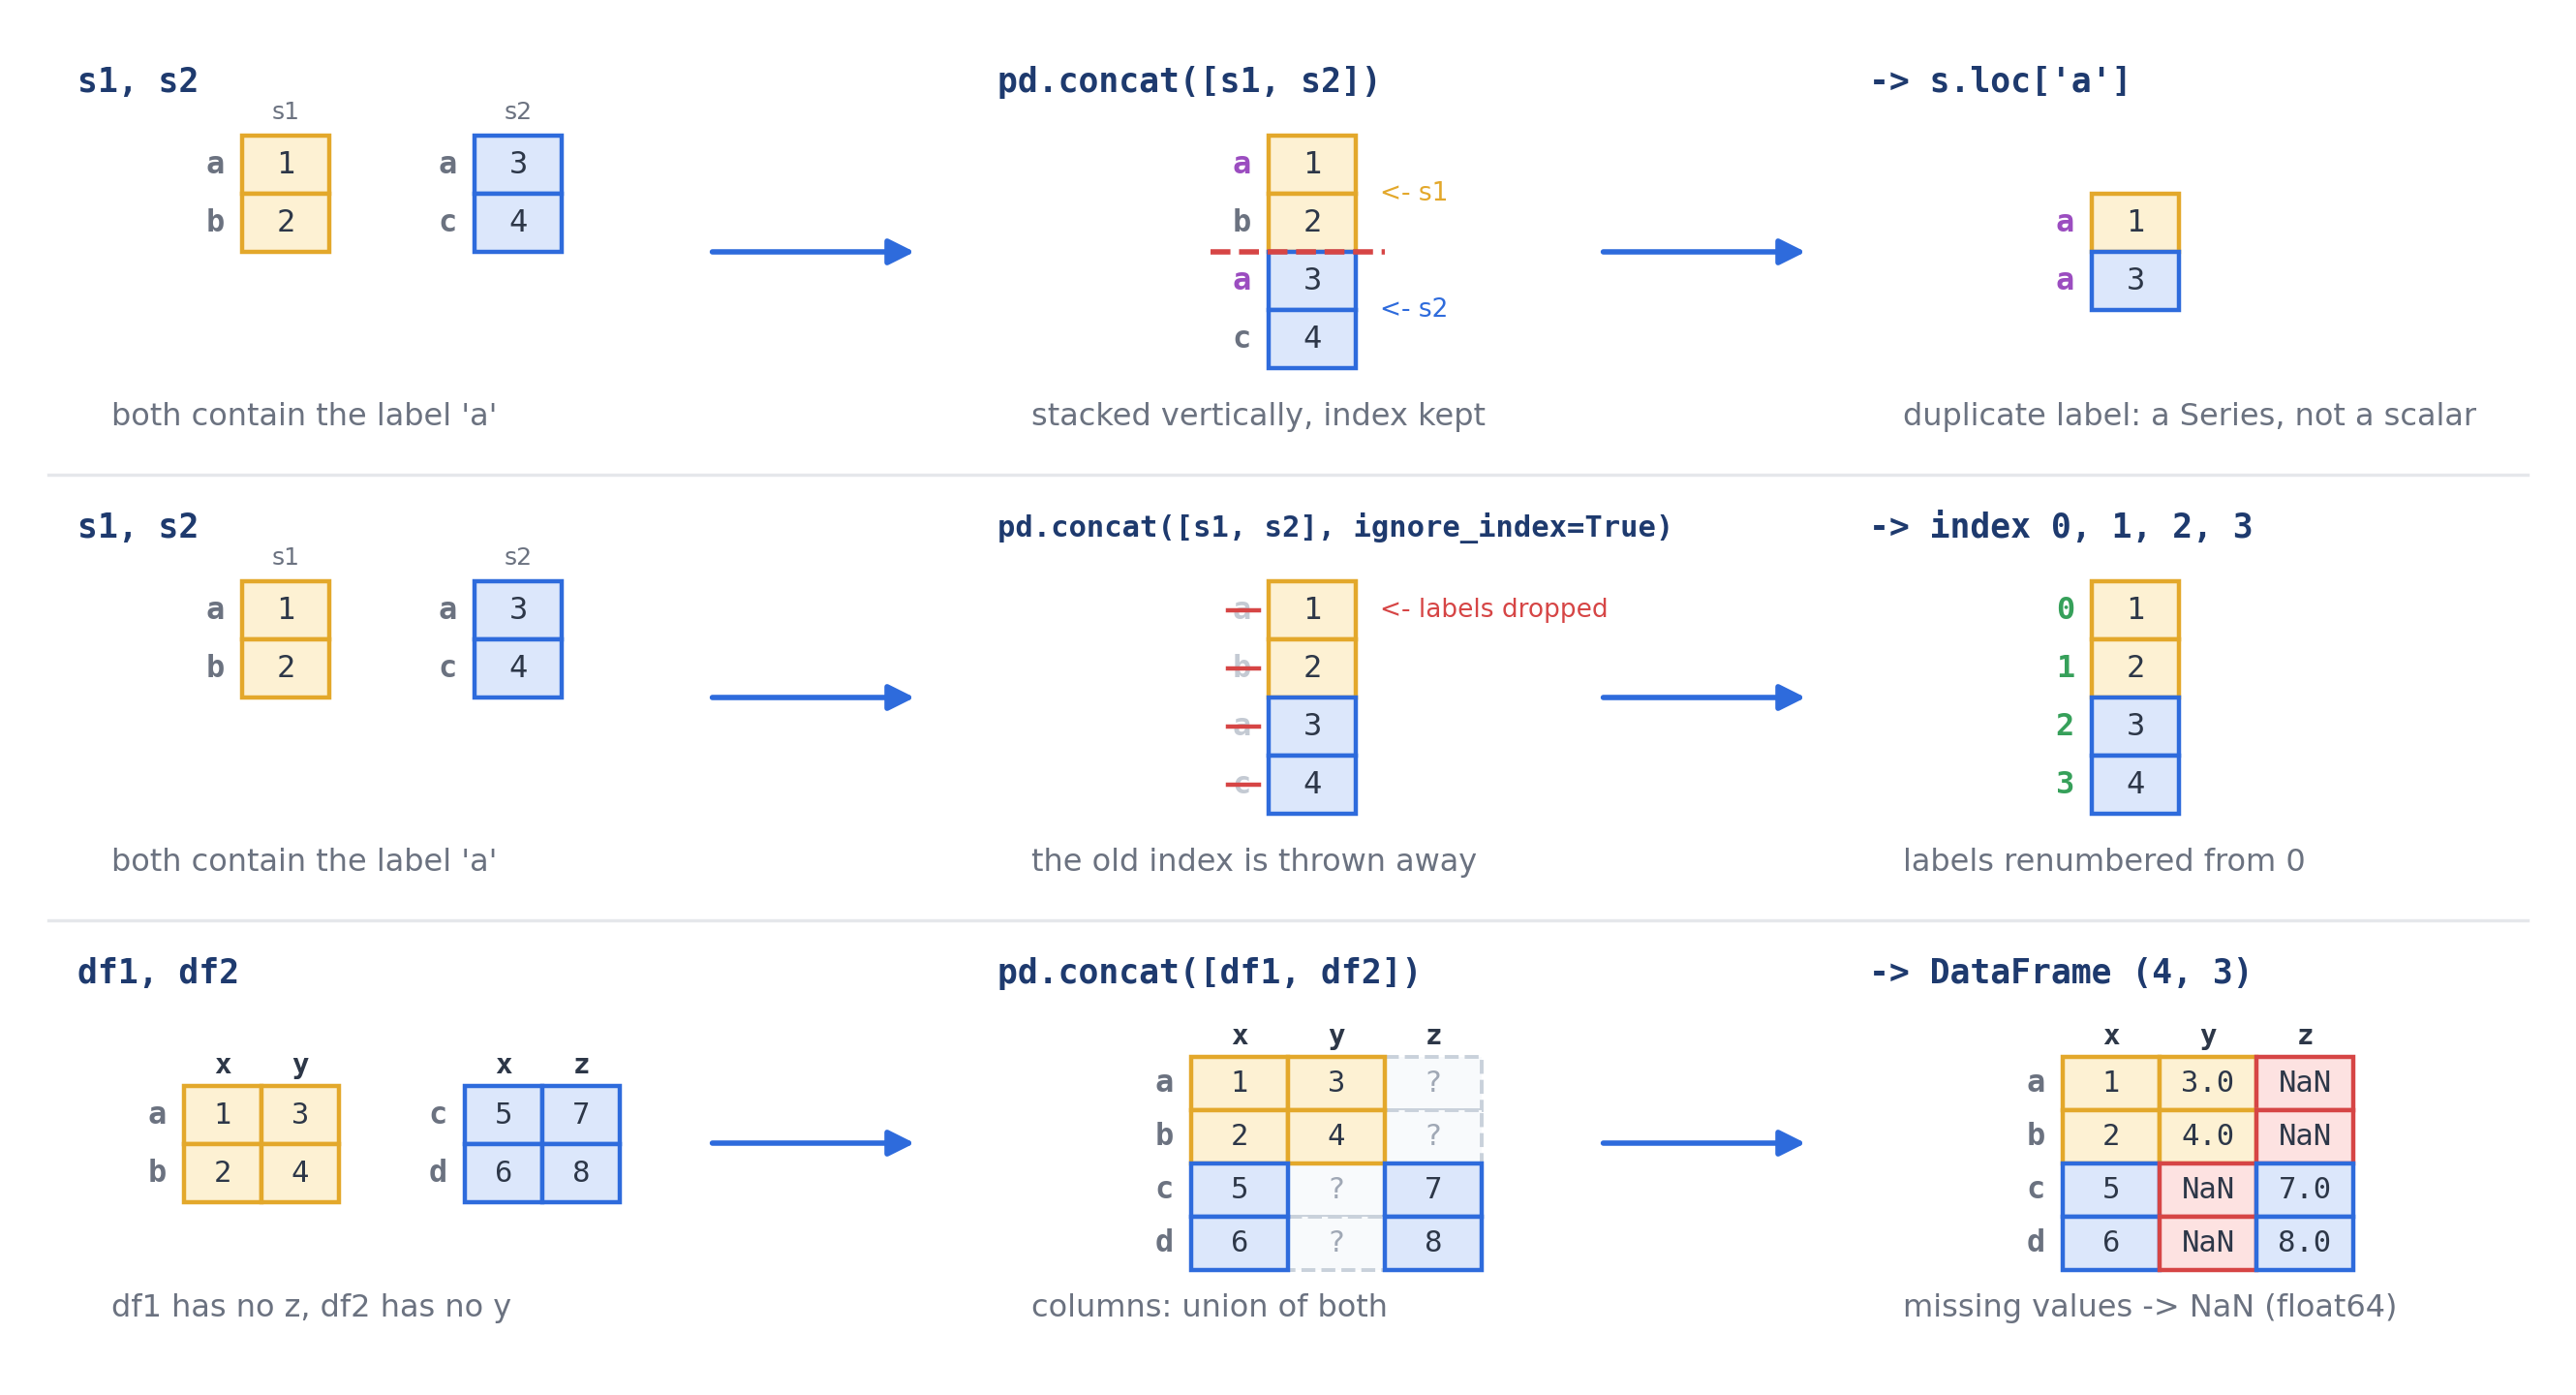
\includegraphics[width=1\textwidth]{contents/images/pandas/sub_concat.png}
    \caption{Concatenation: \texttt{pd.concat} stacks the objects and keeps their labels, so a duplicated label returns several values with \texttt{.loc}. With \texttt{ignore\_index=True} the result is renumbered from 0. Columns missing in one DataFrame are filled with \texttt{NaN}.}
\end{figure}

\begin{itemize}
    \item \textbf{Index preservation:} Concatenation keeps the original index as it is, including duplicate labels. If a label is duplicated, selecting it via \texttt{.loc} will return a Series containing all matches instead of a single scalar.
    \item \textbf{Resetting the index:} Passing \texttt{ignore\_index=True} throws the old index away and renumbers the elements sequentially.
    \item \textbf{Missing columns:} When concatenating DataFrames, if one DataFrame lacks a column present in the other, pandas fills the missing values with \texttt{NaN}.
\end{itemize}

\textit{Note:} The old \texttt{df1.append(df2)} method was removed in pandas 2.0; you should always use \texttt{pd.concat} instead.

\subsection{Merge: Joining on Common Values}
\texttt{pd.merge(df1, df2)} combines two DataFrames similarly to a database SQL join.

\begin{figure}[h]
    \centering
    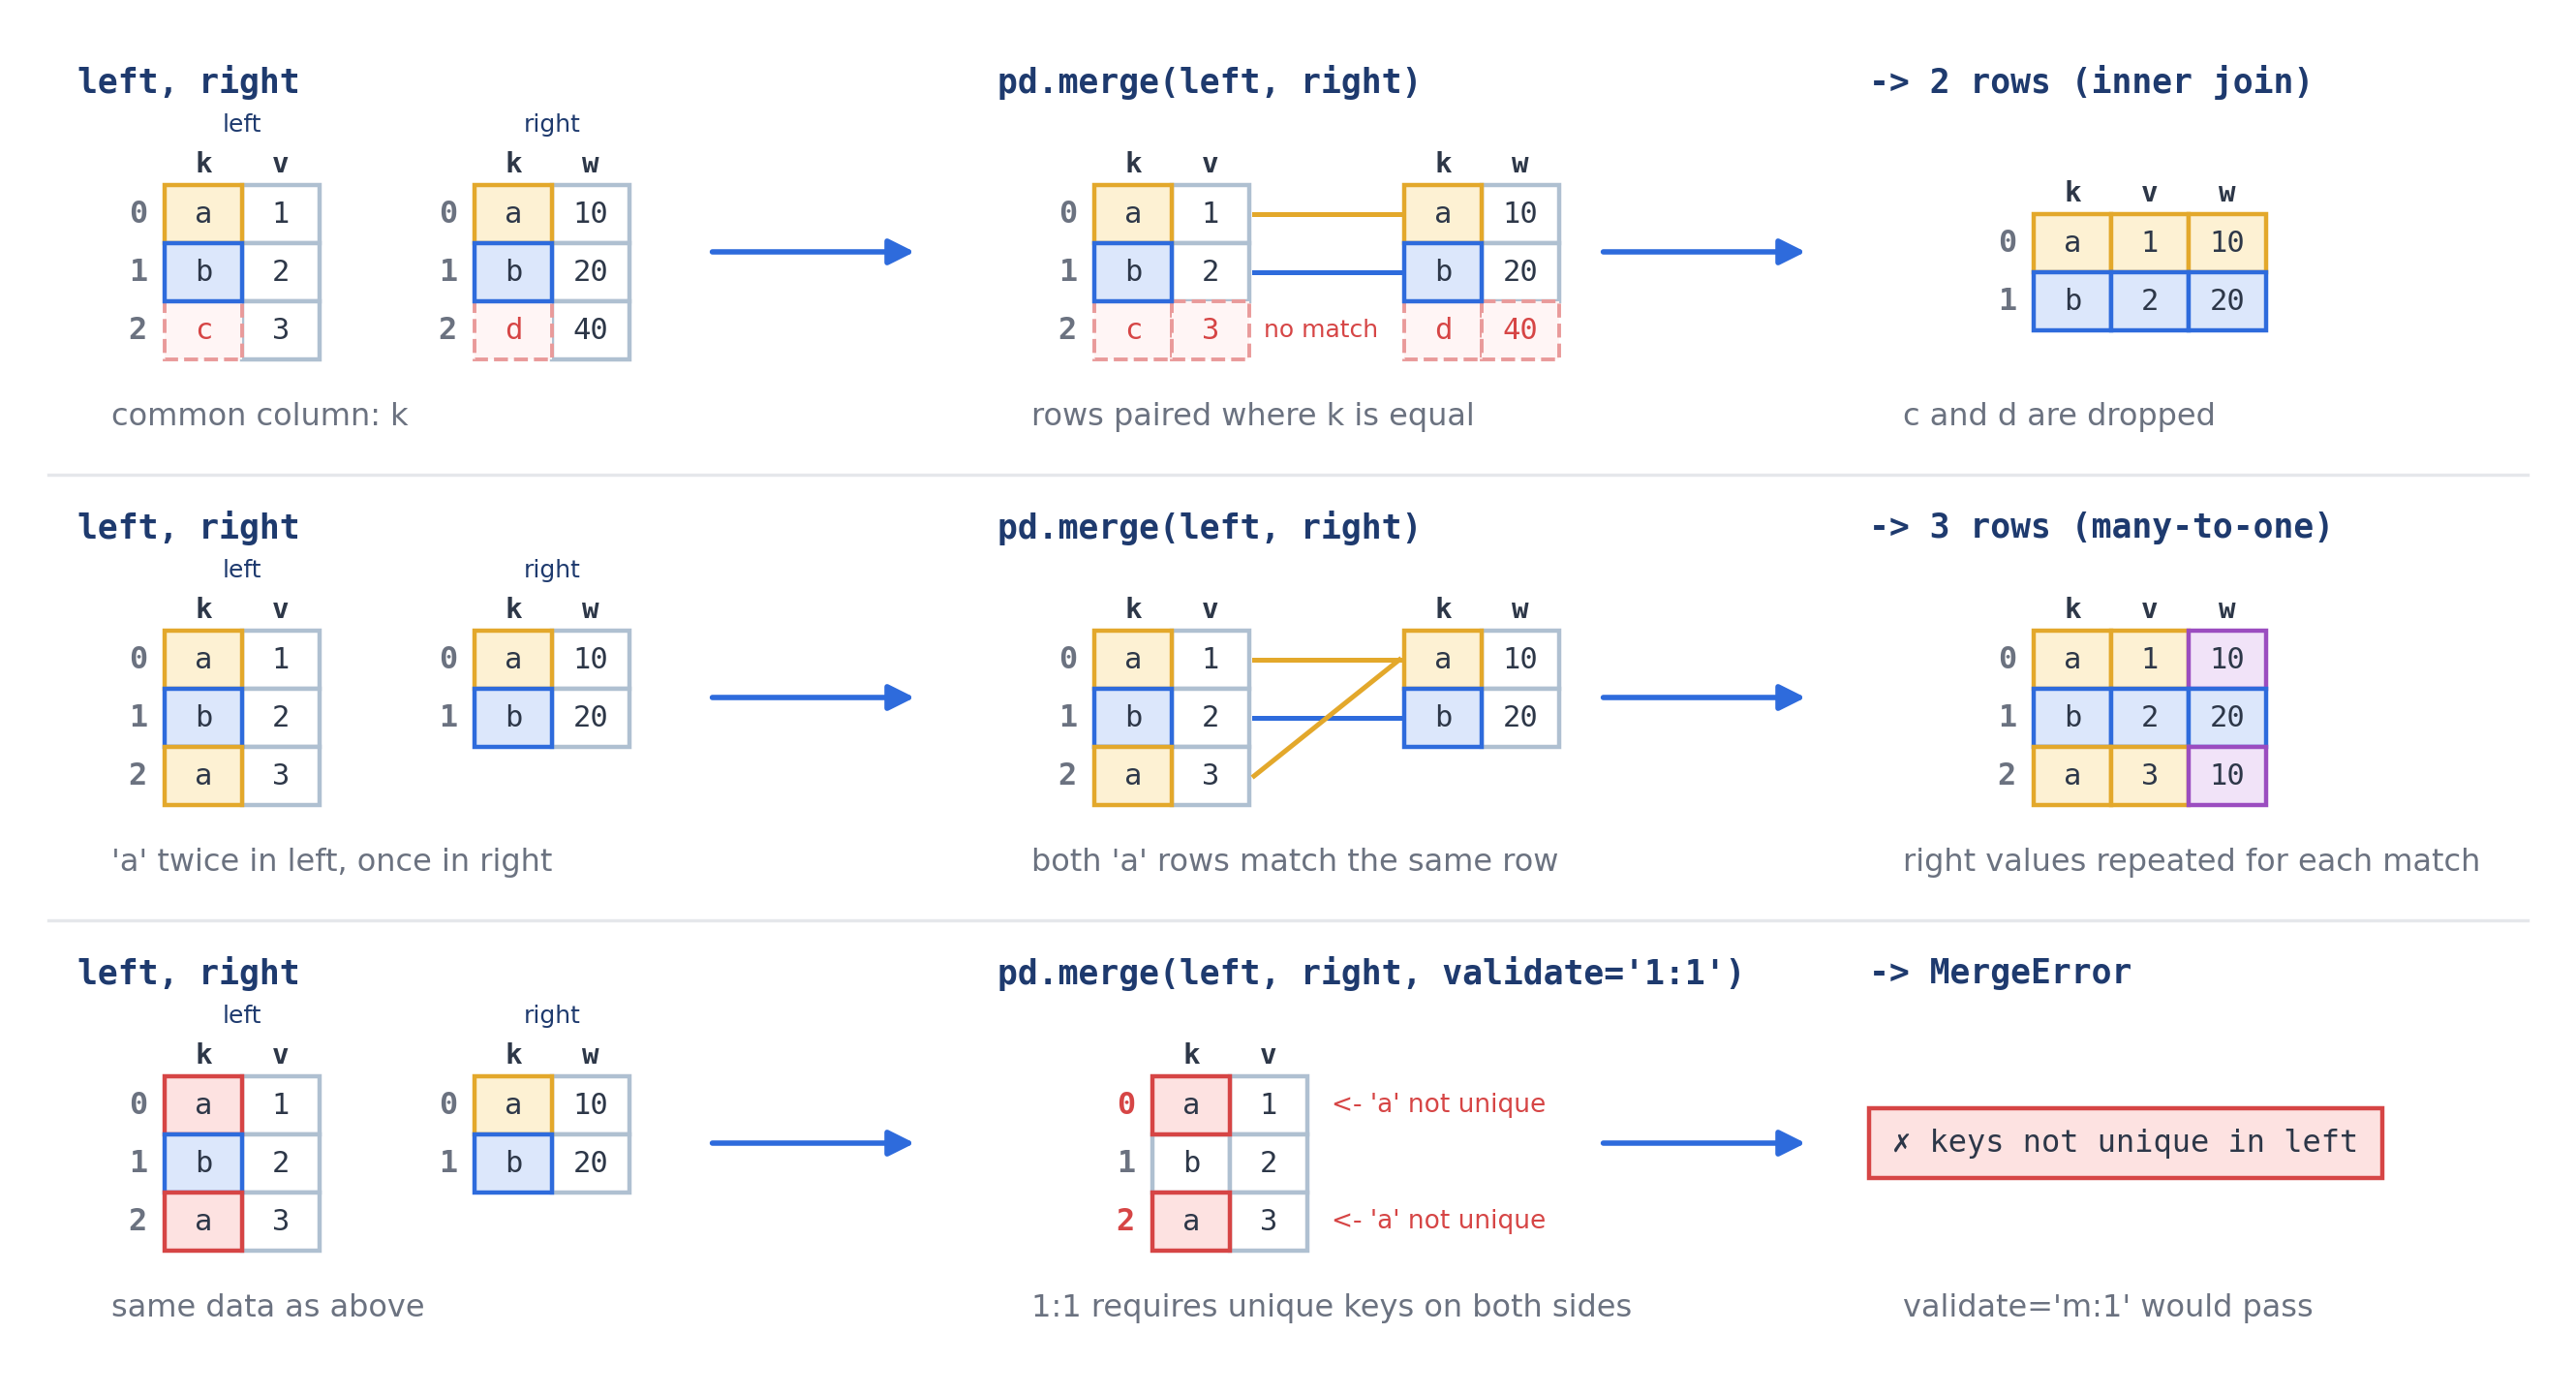
\includegraphics[width=1\textwidth]{contents/images/pandas/sub_merge.png}
    \caption{Merge: rows are paired where the key column \texttt{k} has the same value; by default (inner join) unmatched rows are dropped. In a many-to-one merge the right values are repeated for every matching left row. \texttt{validate='1:1'} raises a \texttt{MergeError} when the keys are not unique.}
\end{figure}

\begin{itemize}
    \item It pairs rows that share equal values in specific columns (by default, columns with the same name, or specified explicitly via \texttt{on=}).
    \item You can also join based on indices using \texttt{left\_index=True, right\_index=True}.
    \item It supports one-to-one, many-to-one, and many-to-many joins. In a many-to-one join, values from the right DataFrame are repeated to match the left.
    \item The \texttt{validate} argument (e.g., \texttt{validate='1:1'}) is used to verify the expected merge type and will raise an error if the data violates this expectation.
\end{itemize}

\lstinputlisting[caption={Concatenating and merging pandas objects.}]{contents/listings/pandas/pandas_combining.py}



\section{Grouping Data}
Pandas provides the equivalent of the SQL \texttt{GROUP BY} statement via \texttt{df.groupby(...)}. This allows you to split the rows into groups by the value of a key column, then iterate, aggregate, or filter the groups.

\subsection{The GroupBy Mechanism}
\begin{figure}[h]
    \centering
    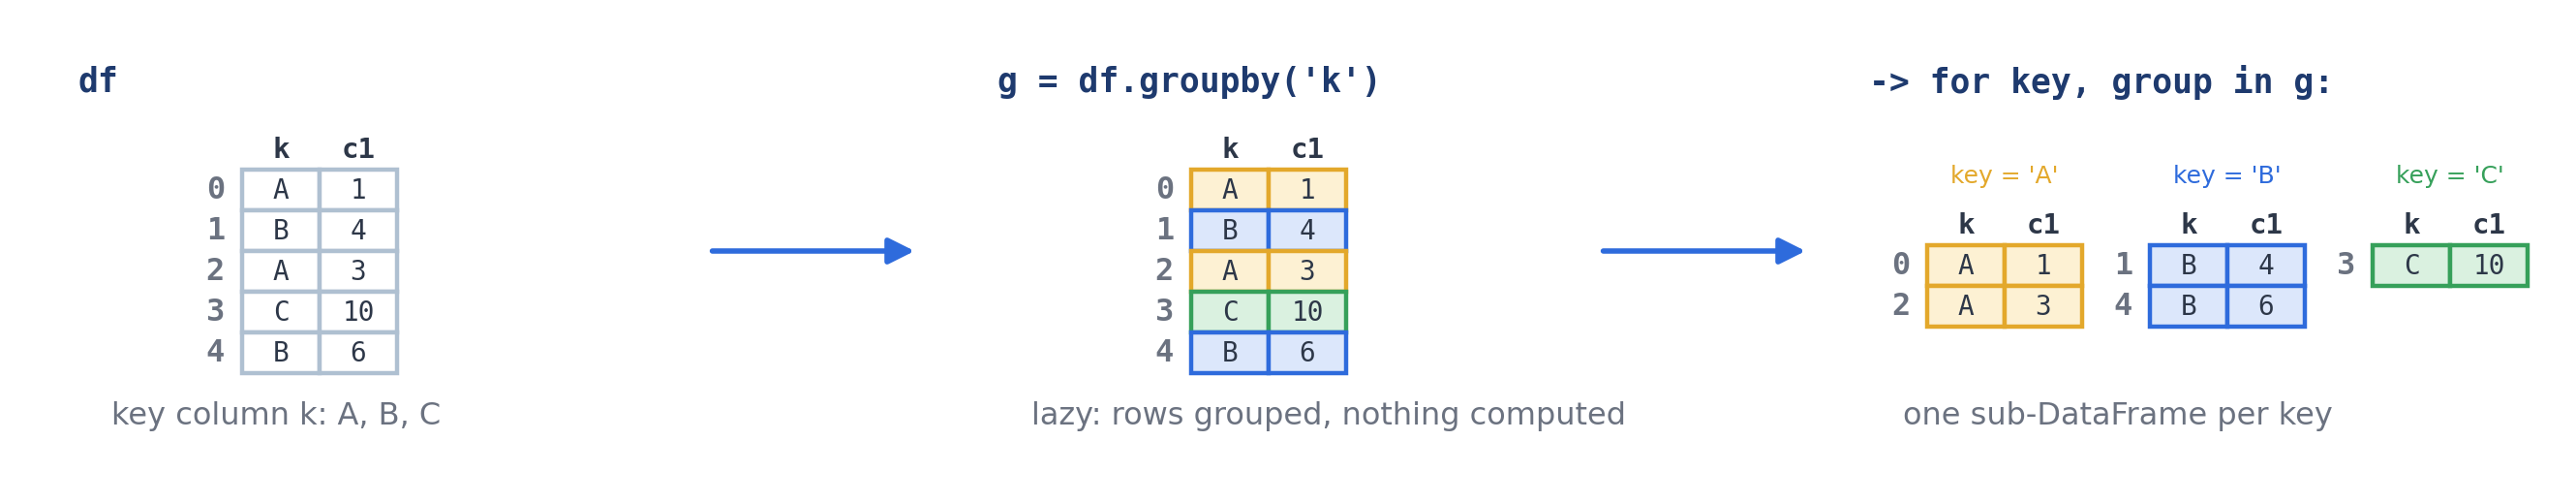
\includegraphics[width=1\textwidth]{contents/images/pandas/sub_groupby_mechanism.png}
    \caption{The GroupBy mechanism: \texttt{df.groupby('k')} only records which rows belong to each key, without computing anything. Iterating over it yields one \texttt{(key, sub-DataFrame)} pair per group, with the original row labels.}
\end{figure}

Calling \texttt{df.groupby("k")} returns a \texttt{DataFrameGroupBy} object, not a computed table; no computation occurs until you explicitly ask for it. You can iterate over this object in a loop, which yields pairs of the group key and a DataFrame subset containing only that group's rows.

\subsection{Aggregating by Group}
When you aggregate a grouped object, the result contains one row per group, and the grouping key becomes the new index.

\begin{figure}[h]
    \centering
    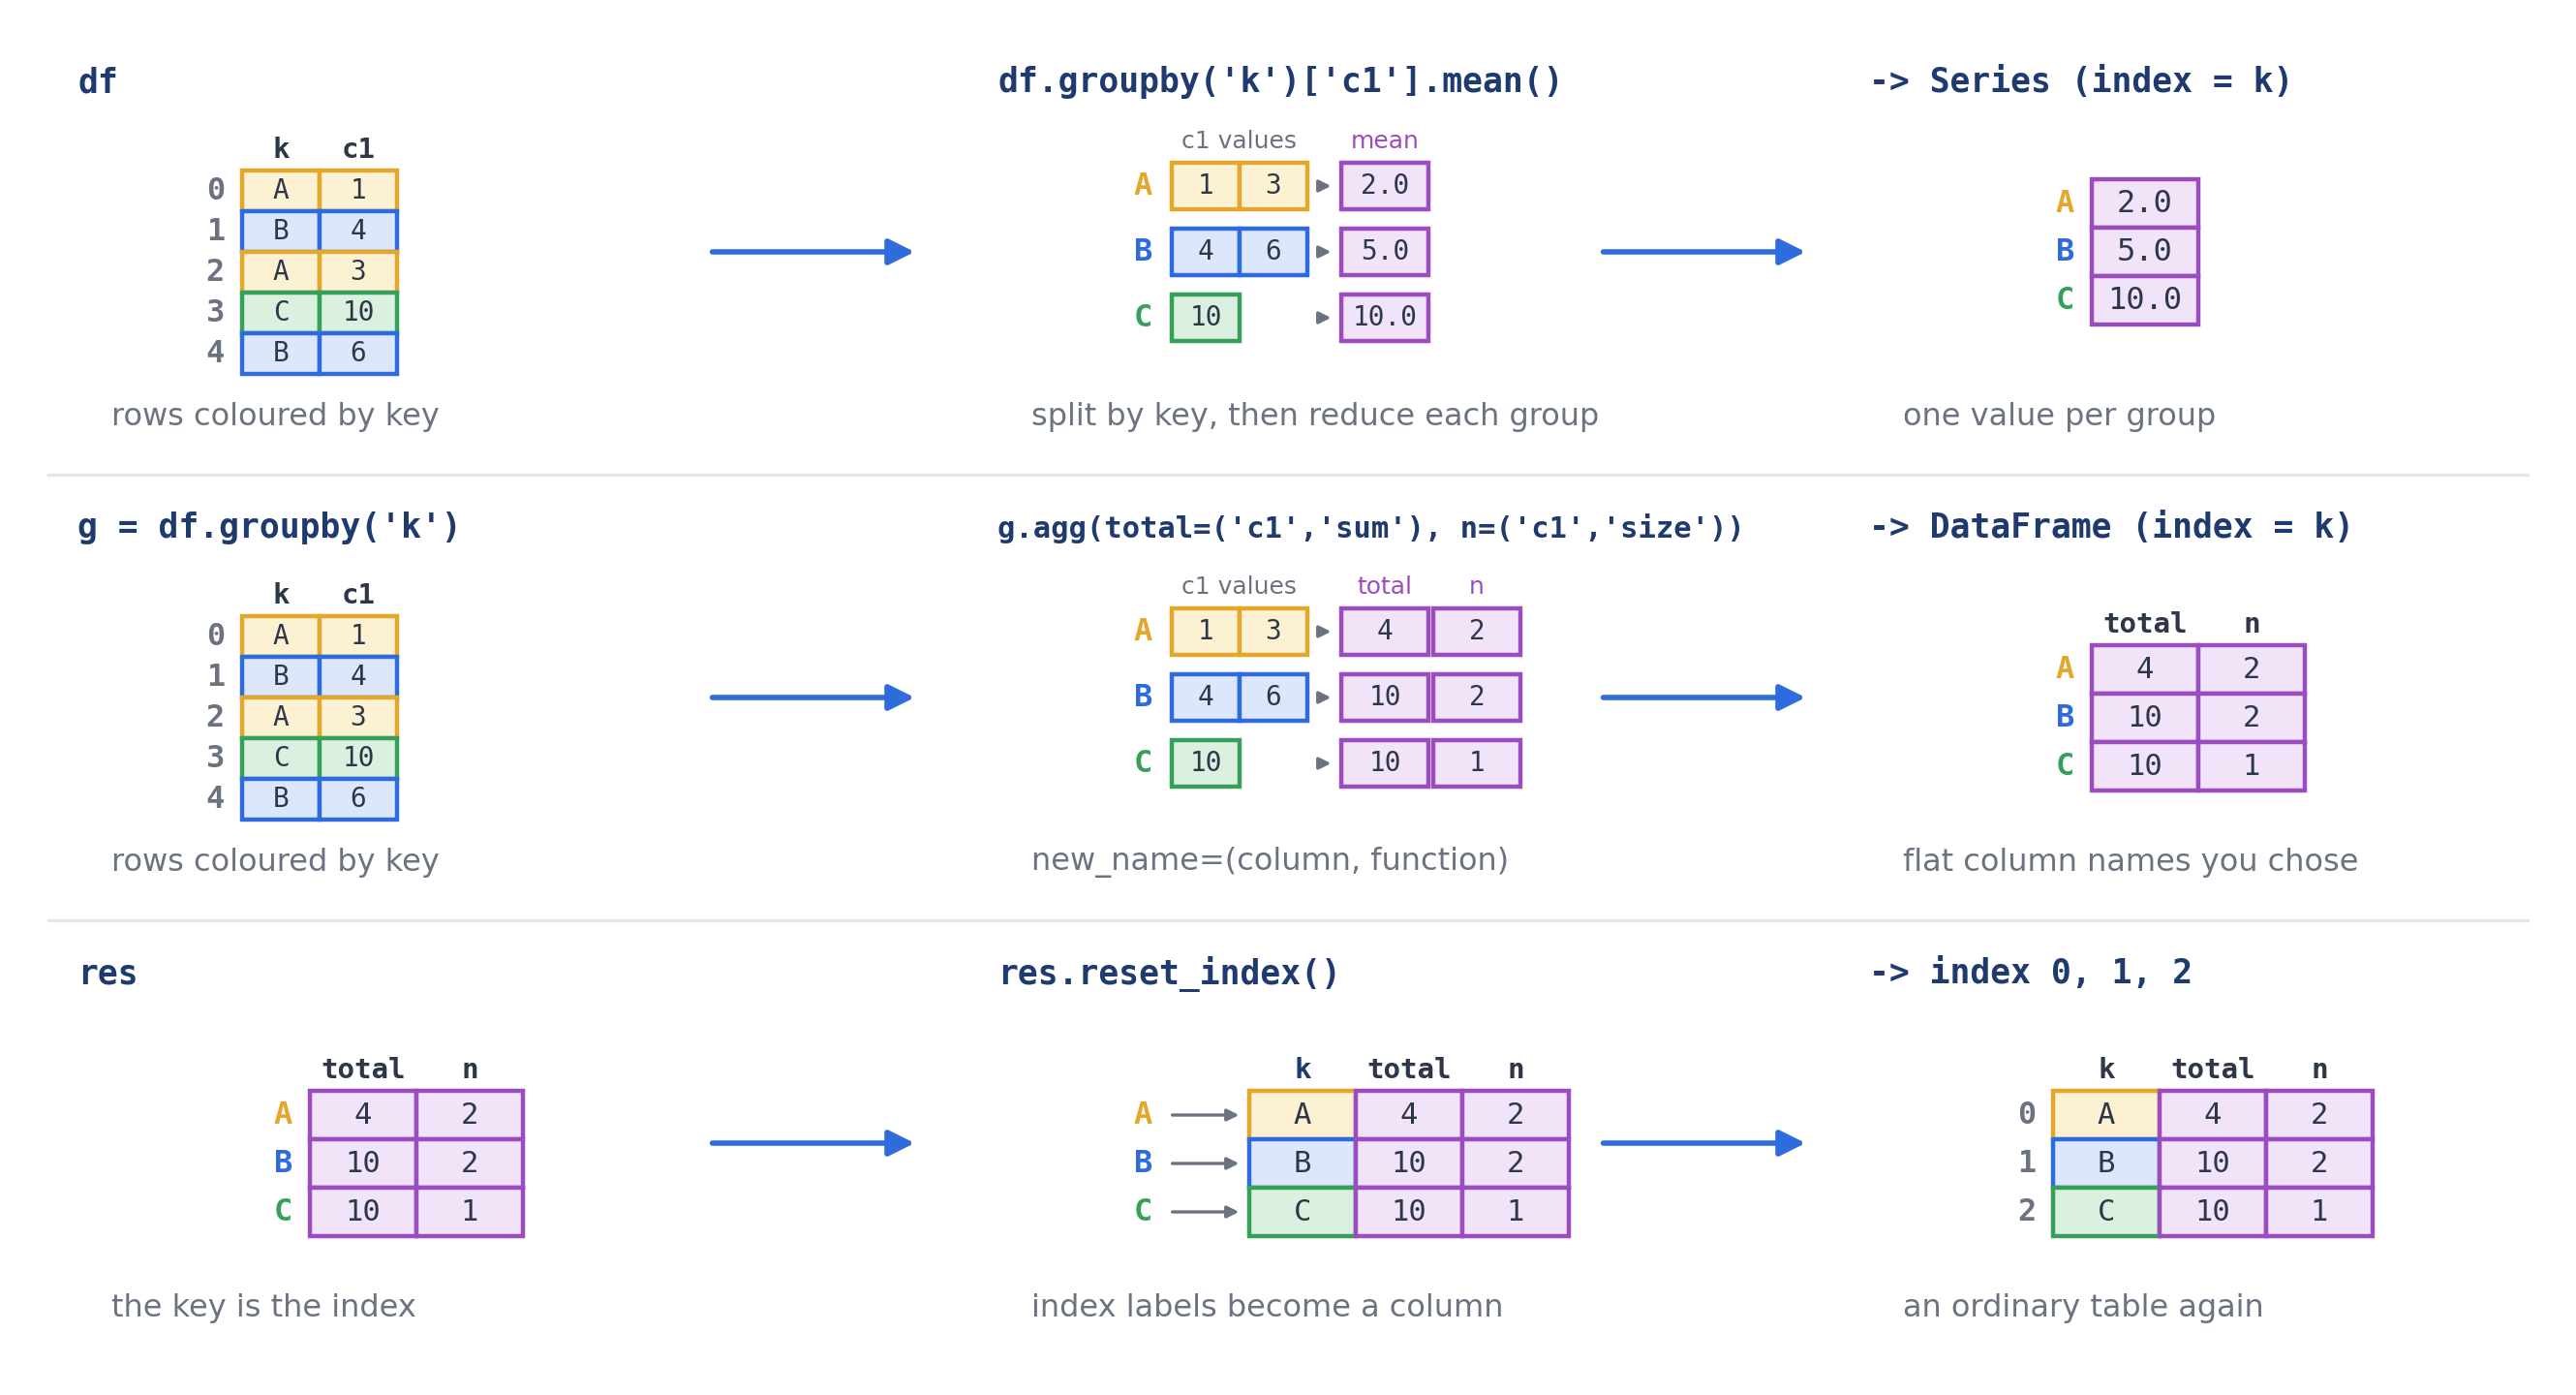
\includegraphics[width=1\textwidth]{contents/images/pandas/sub_groupby_agg.png}
    \caption{Aggregating by group: each group is reduced to one row and the key becomes the index. Named aggregation (\texttt{new\_name=(column, function)}) gives flat column names, and \texttt{reset\_index()} turns the key back into an ordinary column.}
\end{figure}

\begin{itemize}
    \item \textbf{Single column:} \texttt{df.groupby('k')['c1'].mean()} returns a Series.
    \item \textbf{All columns:} \texttt{df.groupby('k').mean()} applies the function to every numeric column and returns a DataFrame.
    \item \textbf{Resetting the index:} Appending \texttt{.reset\_index()} turns the grouping key back into an ordinary column, replacing the index with a standard $0, 1, 2\dots$ sequence.
    \item \textbf{Named Aggregation (Best Practice):} When performing multiple aggregations via \texttt{.agg()}, pandas creates multi-level column names. To avoid this, use named aggregations: \texttt{.agg(new\_name=('column', 'function'))} to keep a flat, readable table.
\end{itemize}

\subsection{Filtering Groups}
The \texttt{.filter()} method applies a boolean function to each group. It evaluates the entire group as a DataFrame and either keeps or drops the \textit{whole} group. The output consists of the original rows that passed the test, without collapsing them into a single row per group.

\begin{figure}[h]
    \centering
    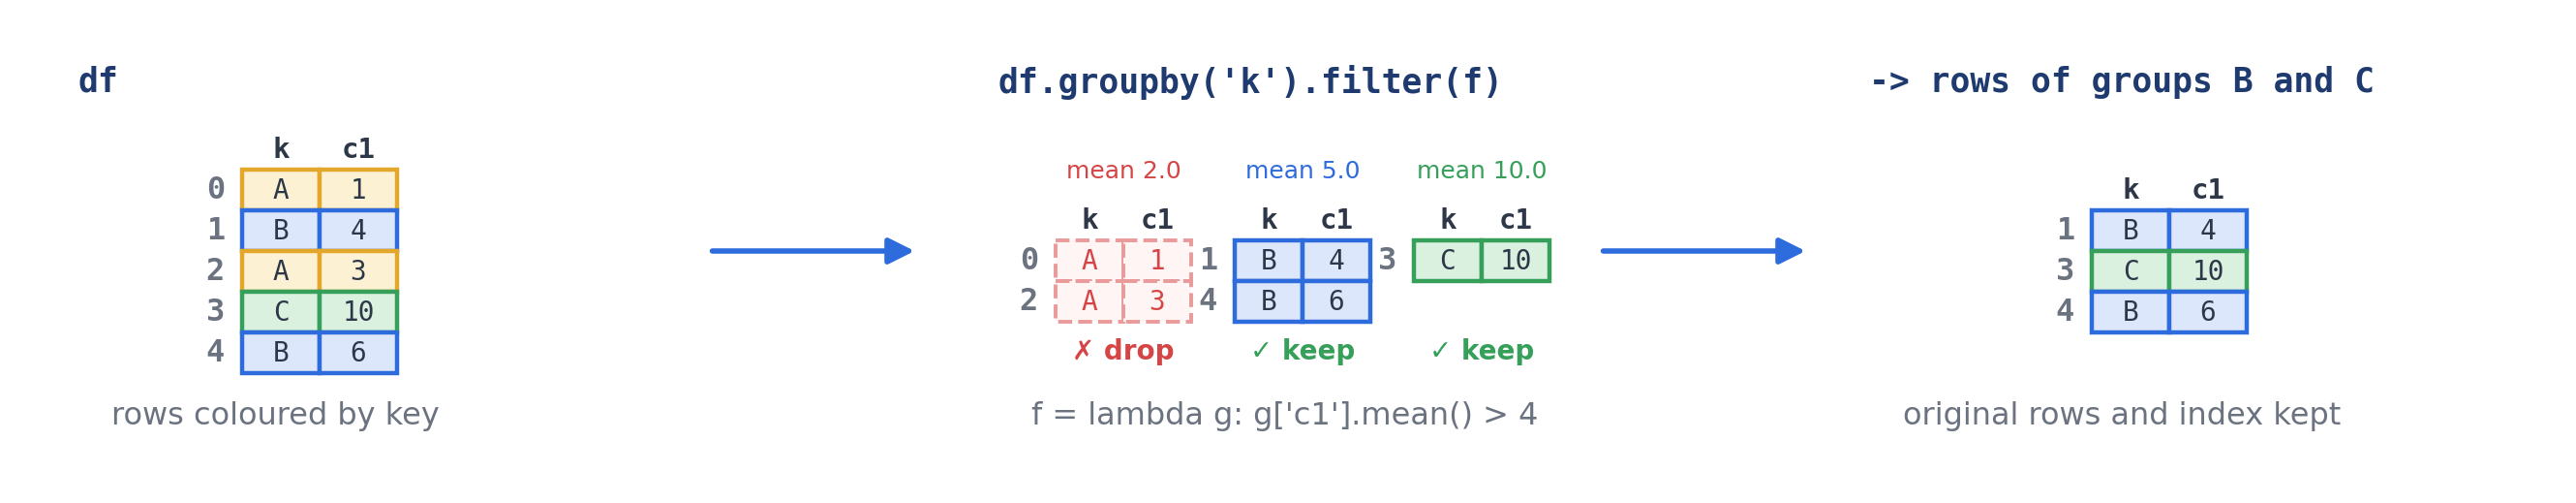
\includegraphics[width=1\textwidth]{contents/images/pandas/sub_groupby_filter.png}
    \caption{Filtering groups: the function receives each group as a DataFrame and returns a single boolean. Whole groups are kept or dropped, and the result contains the original rows with their original index.}
\end{figure}

\lstinputlisting[caption={Grouping, named aggregations, and filtering.}]{contents/listings/pandas/pandas_grouping.py}



\section{DataFrames and I/O}

\subsection{Reading and Writing CSV Files}

\begin{figure}[h]
    \centering
    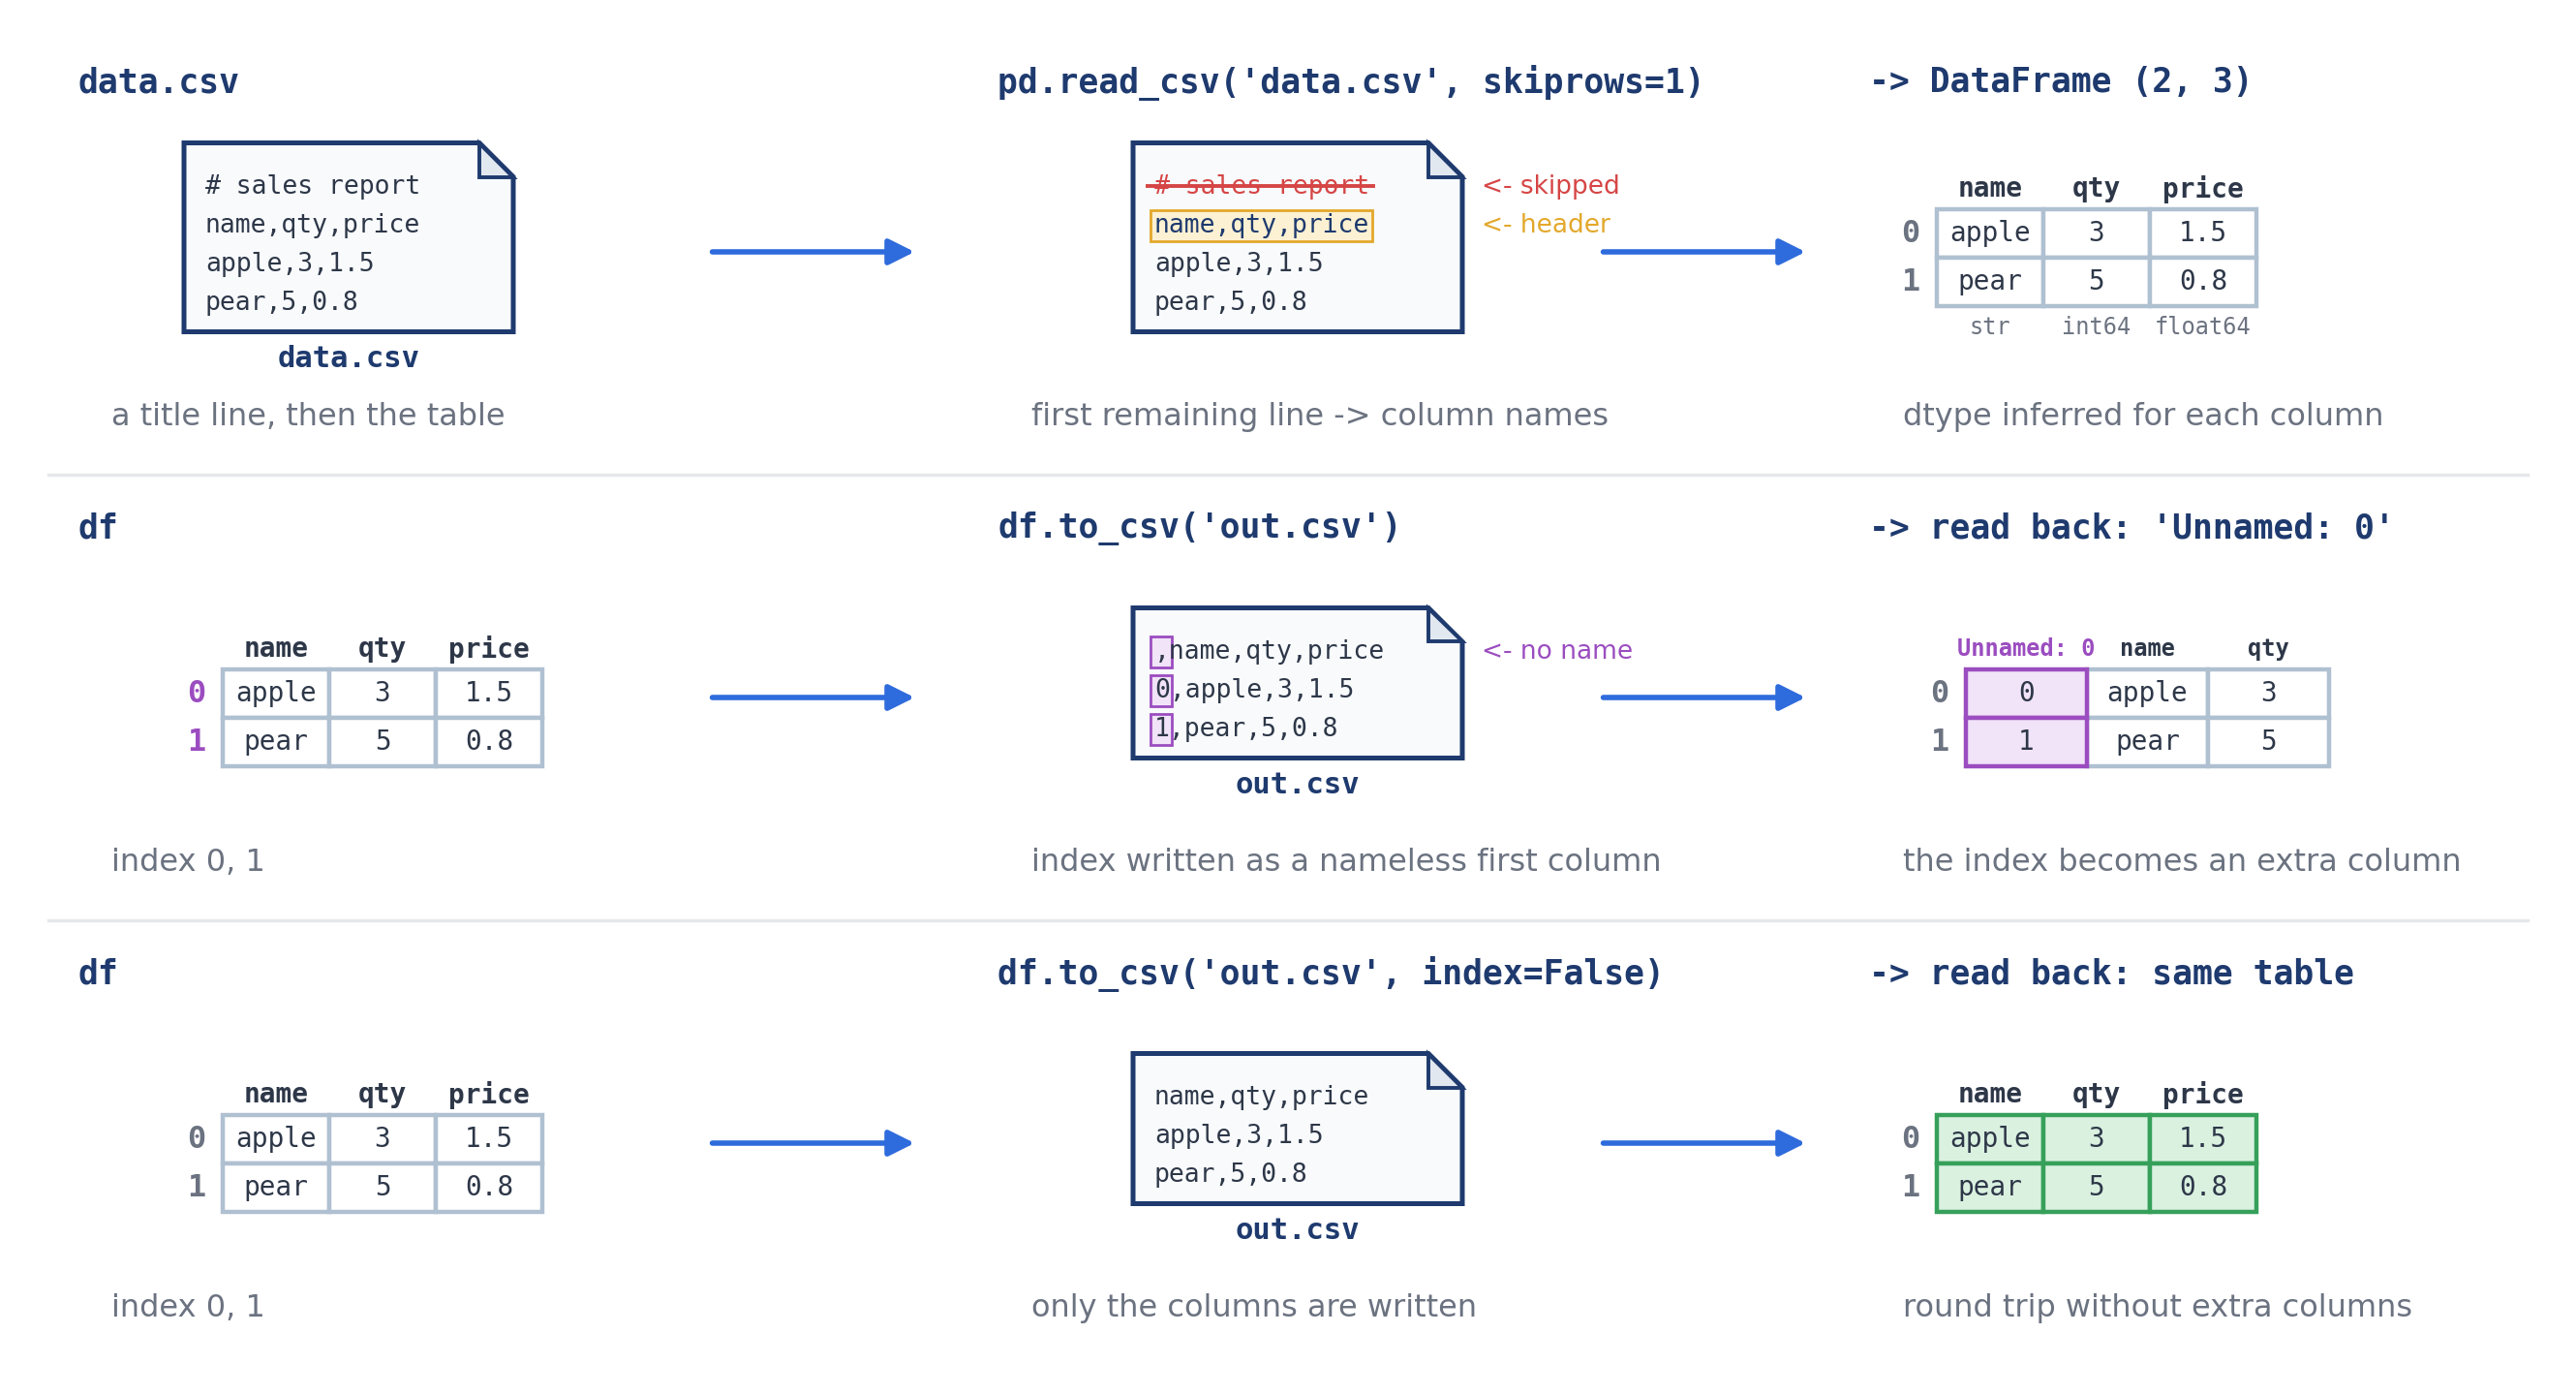
\includegraphics[width=1\textwidth]{contents/images/pandas/sub_csv_io.png}
    \caption{CSV input and output: \texttt{read\_csv} takes the column names from the first line not skipped by \texttt{skiprows} and infers a \texttt{dtype} for each column. By default \texttt{to\_csv} also writes the index as a nameless first column, which comes back as \texttt{Unnamed: 0}; \texttt{index=False} writes only the columns.}
\end{figure}

\begin{itemize}
    \item \textbf{Reading:} \texttt{pd.read\_csv(path, sep=',')} automatically reads column names from the first line and infers the data type of each column. Use \texttt{skiprows=N} to ignore file headers or titles.
    \item \textbf{Writing:} \texttt{df.to\_csv(path)} writes the table to disk. By default, it writes the index as a nameless first column. To omit the index, use \texttt{index=False}.
\end{itemize}

\subsection{Handling Missing Values on Import}
Empty fields and the explicit text "NaN" are automatically converted to \texttt{NaN} upon reading. However, custom missing value markers (e.g., "no info", "x") will cause pandas to read the entire column as text (dtype \texttt{str} or \texttt{object}). To properly parse these and retain numeric types, provide a list of custom markers to the \texttt{na\_values} argument during import.

\begin{figure}[h]
    \centering
    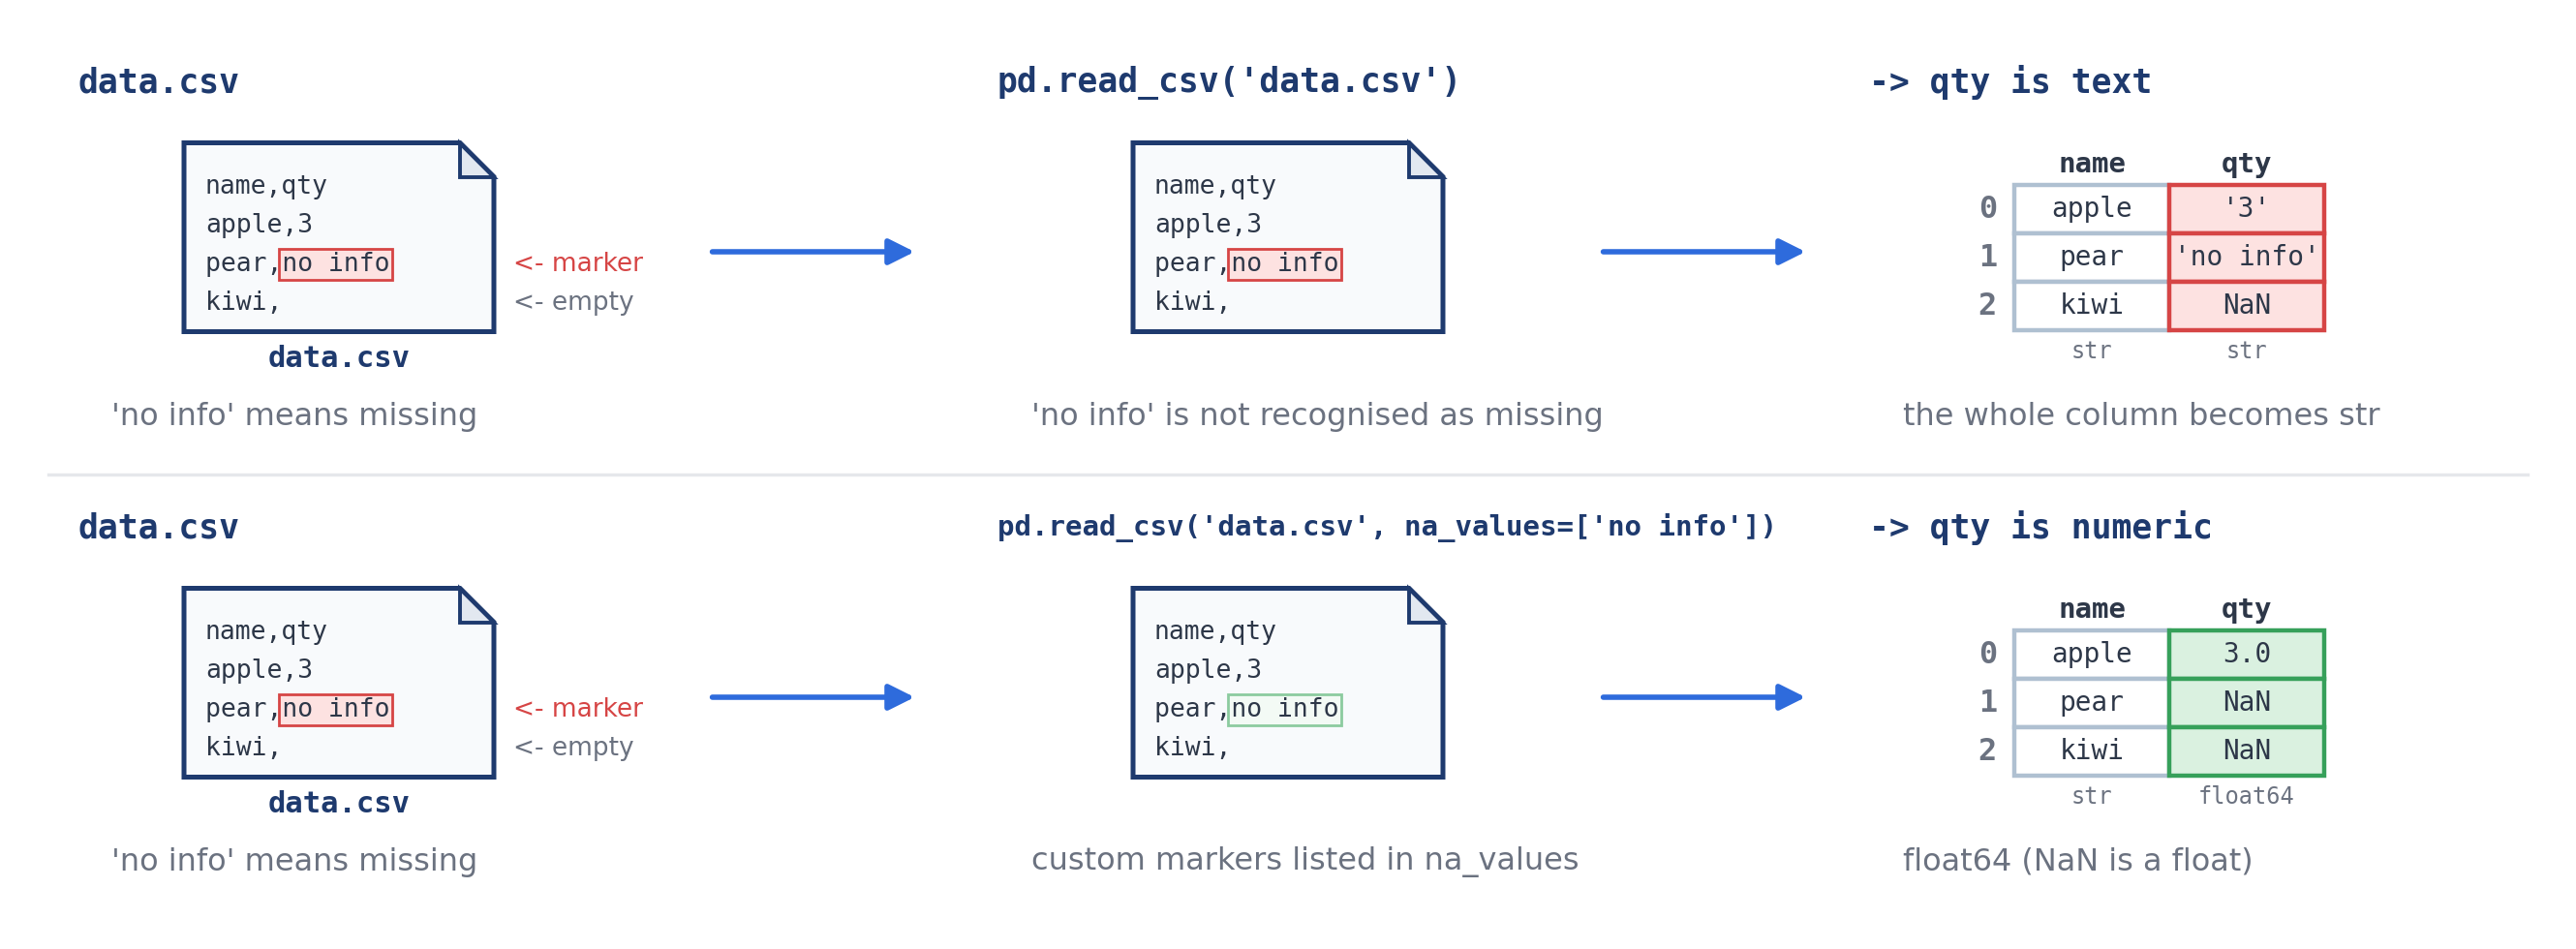
\includegraphics[width=1\textwidth]{contents/images/pandas/sub_missing_values.png}
    \caption{Missing values on import: a custom marker such as \texttt{'no info'} is read as text and turns the whole column into \texttt{str}; listing it in \texttt{na\_values} converts it to \texttt{NaN}, and the column becomes \texttt{float64}.}
\end{figure}

\subsection{Other Supported Formats}
pandas natively supports a wide variety of formats:

\begin{itemize}
    \item \textbf{JSON:} \texttt{pd.read\_json()} and \texttt{df.to\_json}.
    \item \textbf{Excel:} \texttt{pd.read\_excel()} and \texttt{df.to\_excel()}.
    \item \textbf{Parquet:} \texttt{pd.read\_parquet()} and \texttt{df.to\_parquet()} (highly efficient, compressed, and strictly typed, ideal for large datasets).
\end{itemize}

\begin{figure}[h]
    \centering
    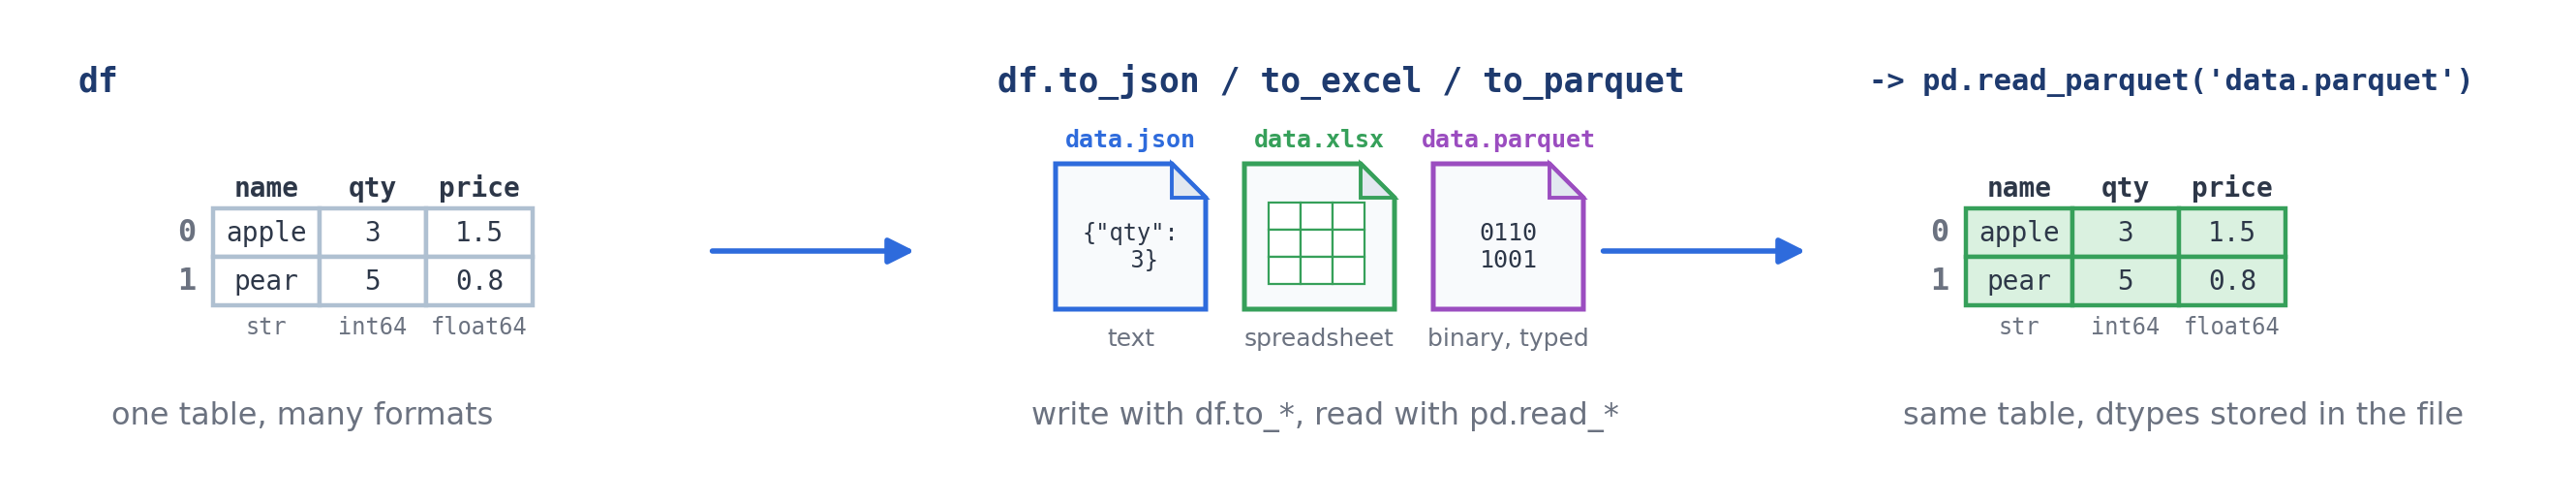
\includegraphics[width=1\textwidth]{contents/images/pandas/sub_formats.png}
    \caption{Other formats: every \texttt{df.to\_*} writer has a matching \texttt{pd.read\_*} reader. JSON is plain text, Excel is a spreadsheet, and Parquet is a compressed binary format that also stores the \texttt{dtype} of each column.}
\end{figure}

\lstinputlisting[caption={Reading and writing CSV files, handling custom missing values.}]{contents/listings/pandas/pandas_io.py}



\section{Missing Values}
Missing data is a common occurrence in real-world datasets (e.g., a sensor failing to answer, an empty field in a file, or a merge with no match). pandas marks these missing values with \texttt{NaN} (Not a Number), and it also accepts standard Python \texttt{None} values, automatically converting them to \texttt{NaN}. 
Because \texttt{NaN} is technically a floating-point value, introducing it into a column of integers will upcast the entire column to \texttt{float64}, allowing the numbers to remain in a highly optimized NumPy array.

\subsection{Detecting, Dropping, and Filling}
pandas provides several methods to handle missing data. It is important to note that \textbf{none of these methods modify the original object}; each returns a new Series or DataFrame.

\begin{figure}[h]
    \centering
    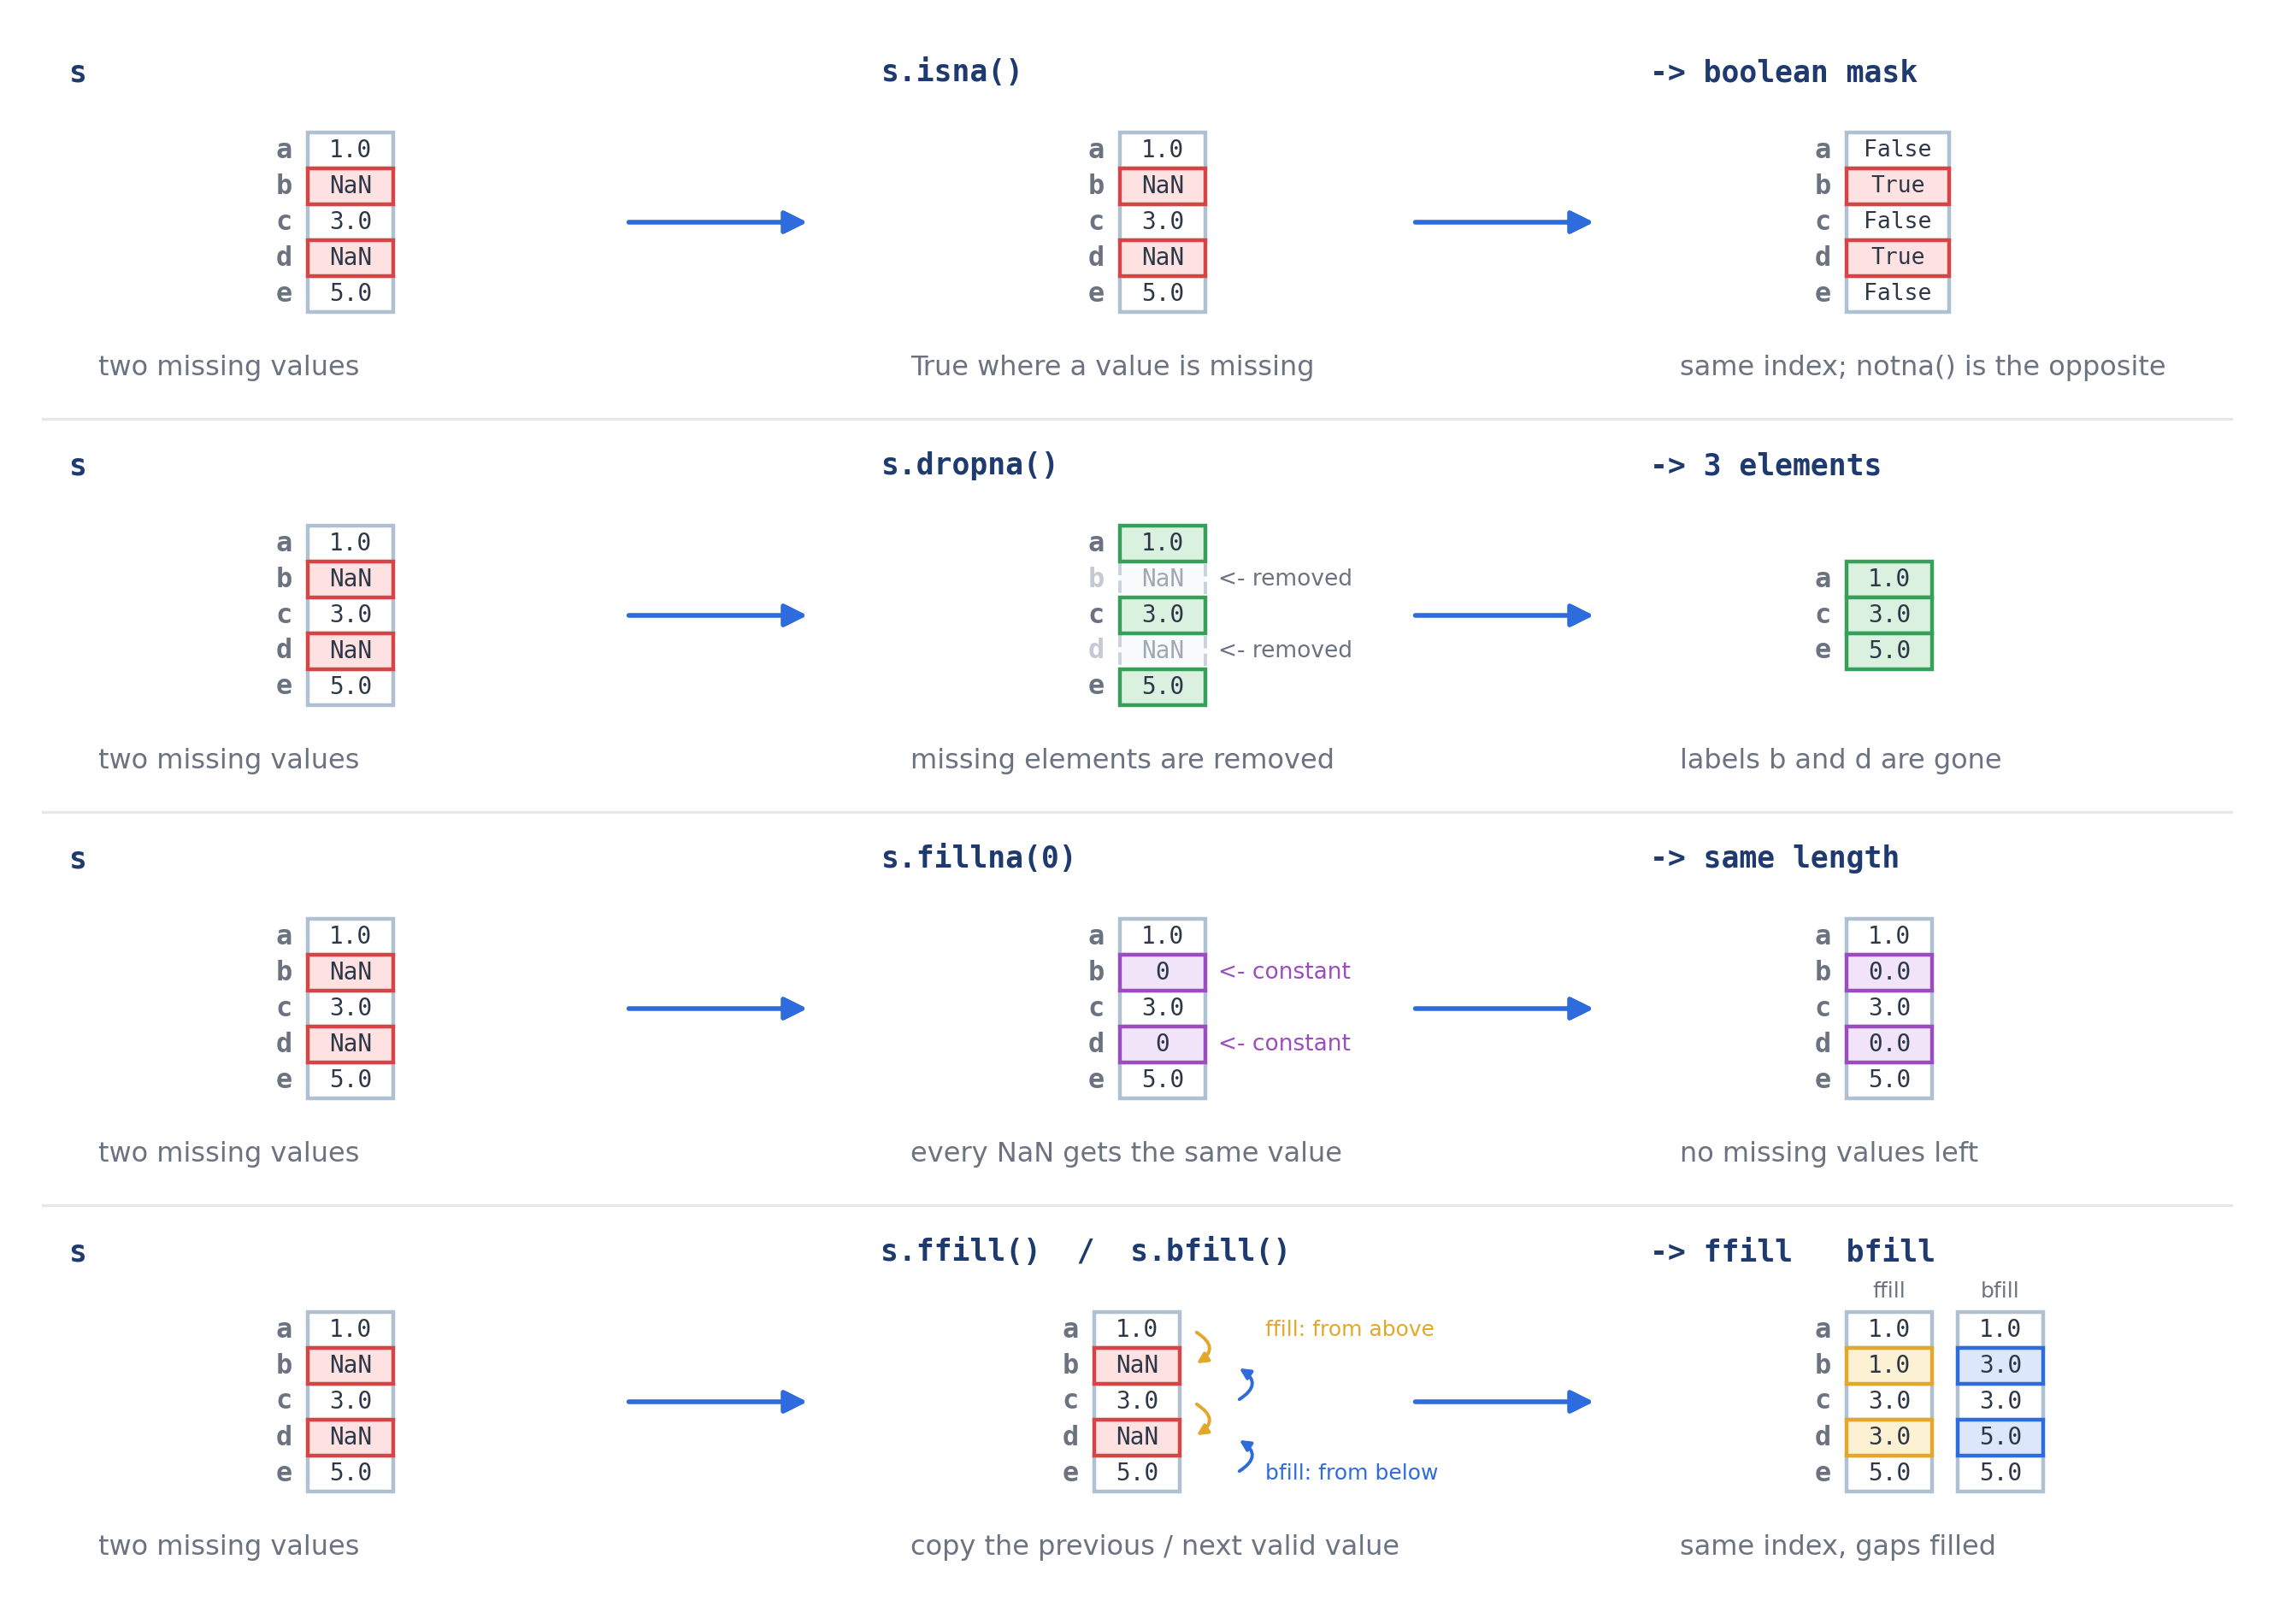
\includegraphics[width=1\textwidth]{contents/images/pandas/sub_missing_series.png}
    \caption{Missing values in a Series: \texttt{isna()} marks them with \texttt{True}, \texttt{dropna()} removes them together with their labels, \texttt{fillna(0)} replaces them with a constant, and \texttt{ffill()}/\texttt{bfill()} copy the previous or next valid value. Each method returns a new object.}
\end{figure}

\begin{itemize}
    \item \textbf{Detecting:} \texttt{isna()} (and its opposite, \texttt{notna()}) returns a boolean mask of the exact same shape, containing \texttt{True} wherever a value is missing.
    \item \textbf{Dropping:} \texttt{dropna()} completely removes the missing elements.
    \item \textbf{Filling with a constant:} \texttt{fillna(value)} replaces every missing value with the specified \texttt{value} (e.g., \texttt{0}).
    \item \textbf{Forward/Backward filling:} \texttt{ffill()} replaces every missing value with the previous valid one, while \texttt{bfill()} uses the next valid one.
\end{itemize}

\subsection{Missing Values in a DataFrame}
When dealing with a 2-dimensional DataFrame, \texttt{dropna()} drops entire rows that contain at least one missing value. 

\begin{figure}[h]
    \centering
    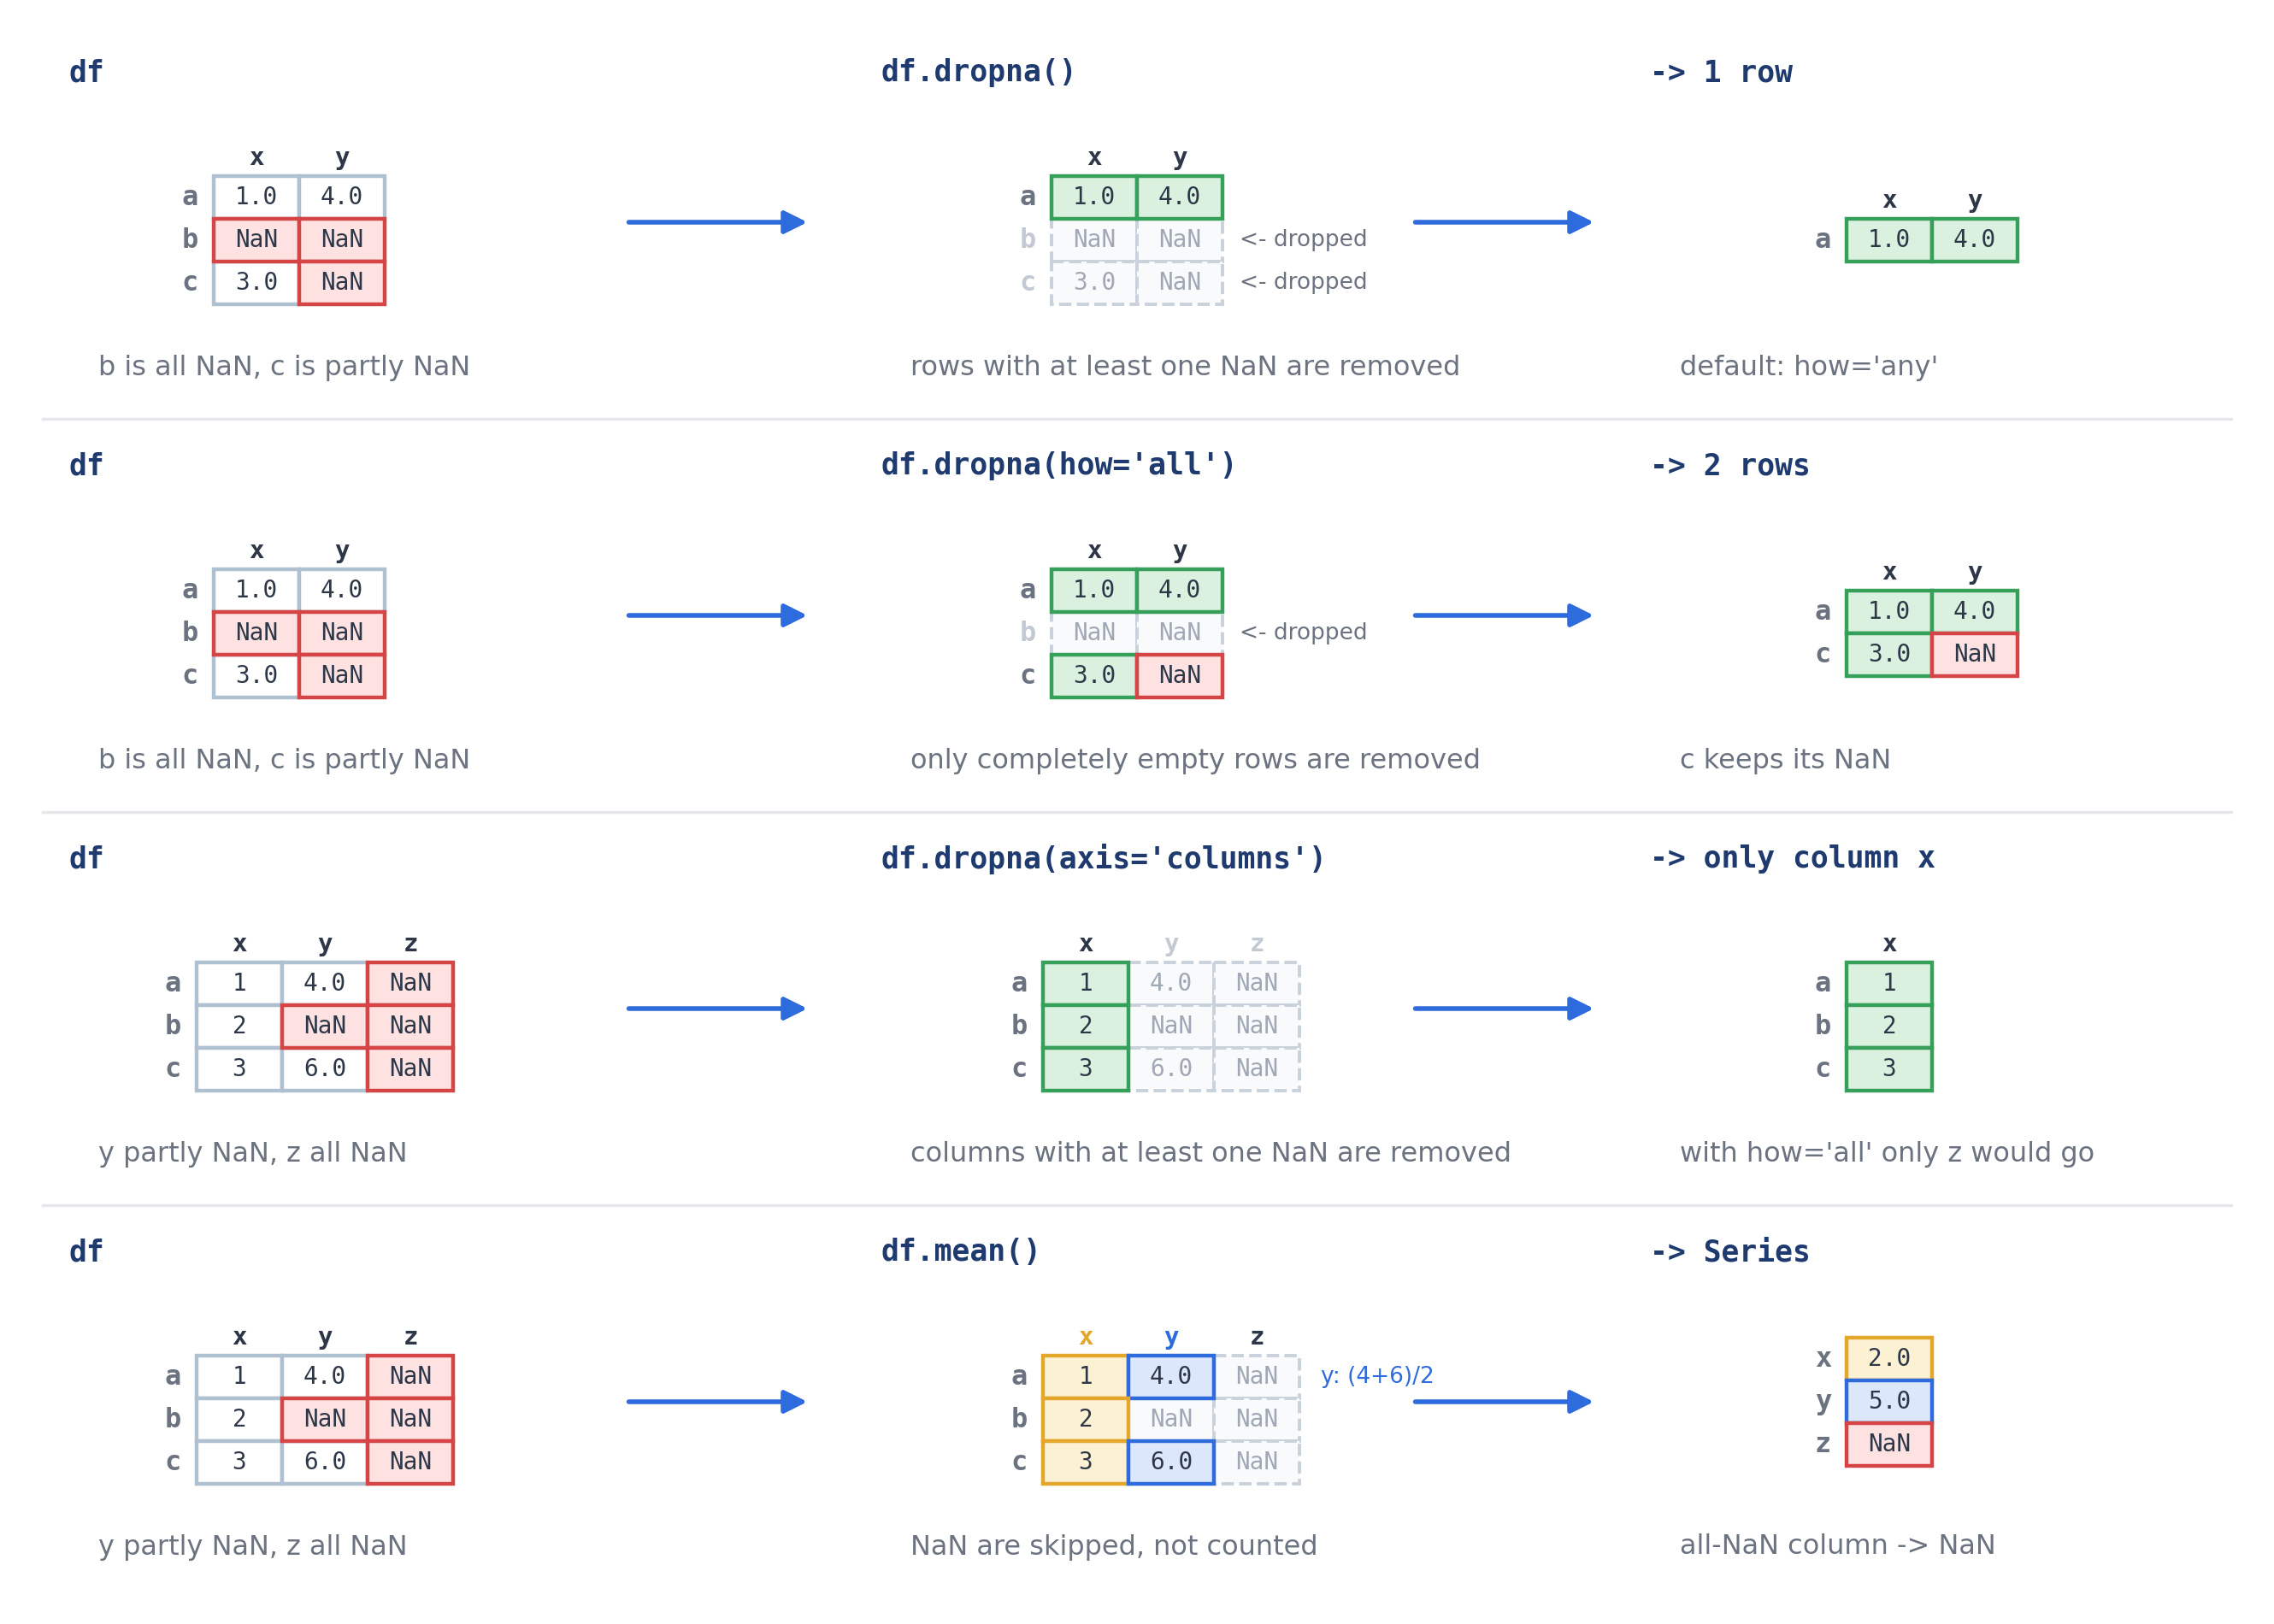
\includegraphics[width=1\textwidth]{contents/images/pandas/sub_missing_dataframe.png}
    \caption{Missing values in a DataFrame: \texttt{dropna()} removes every row with at least one \texttt{NaN}, \texttt{how='all'} only the completely empty ones, and \texttt{axis='columns'} works on columns instead. Aggregations such as \texttt{mean()} skip \texttt{NaN}; a column with no valid values gives \texttt{NaN}.}
\end{figure}

\begin{itemize}
    \item You can change this behavior to drop columns instead by using \texttt{axis='columns'}. 
    \item If you only want to drop rows/columns that are entirely empty, use the \texttt{how='all'} argument.
\end{itemize}
Finally, when performing aggregations (like \texttt{.mean()} or \texttt{.sum()}), pandas automatically skips \texttt{NaN} values by default, computing the result using only the existing data points.

\lstinputlisting[caption={Handling missing values in Series and DataFrames.}]{contents/listings/pandas/pandas_missing_values.py}

\chapter{Matplotlib}

\section{Introduction to Matplotlib}
Matplotlib is the foundational plotting library in Python. It is used extensively on its own, and serves as the underlying drawing engine for pandas and Seaborn. The standard import convention is \texttt{import matplotlib.pyplot as plt}.

\subsection{Two Interfaces: Stateful vs. Stateless}
Matplotlib can be used in two distinct ways[cite: 156]:

\begin{figure}[h]
    \centering
    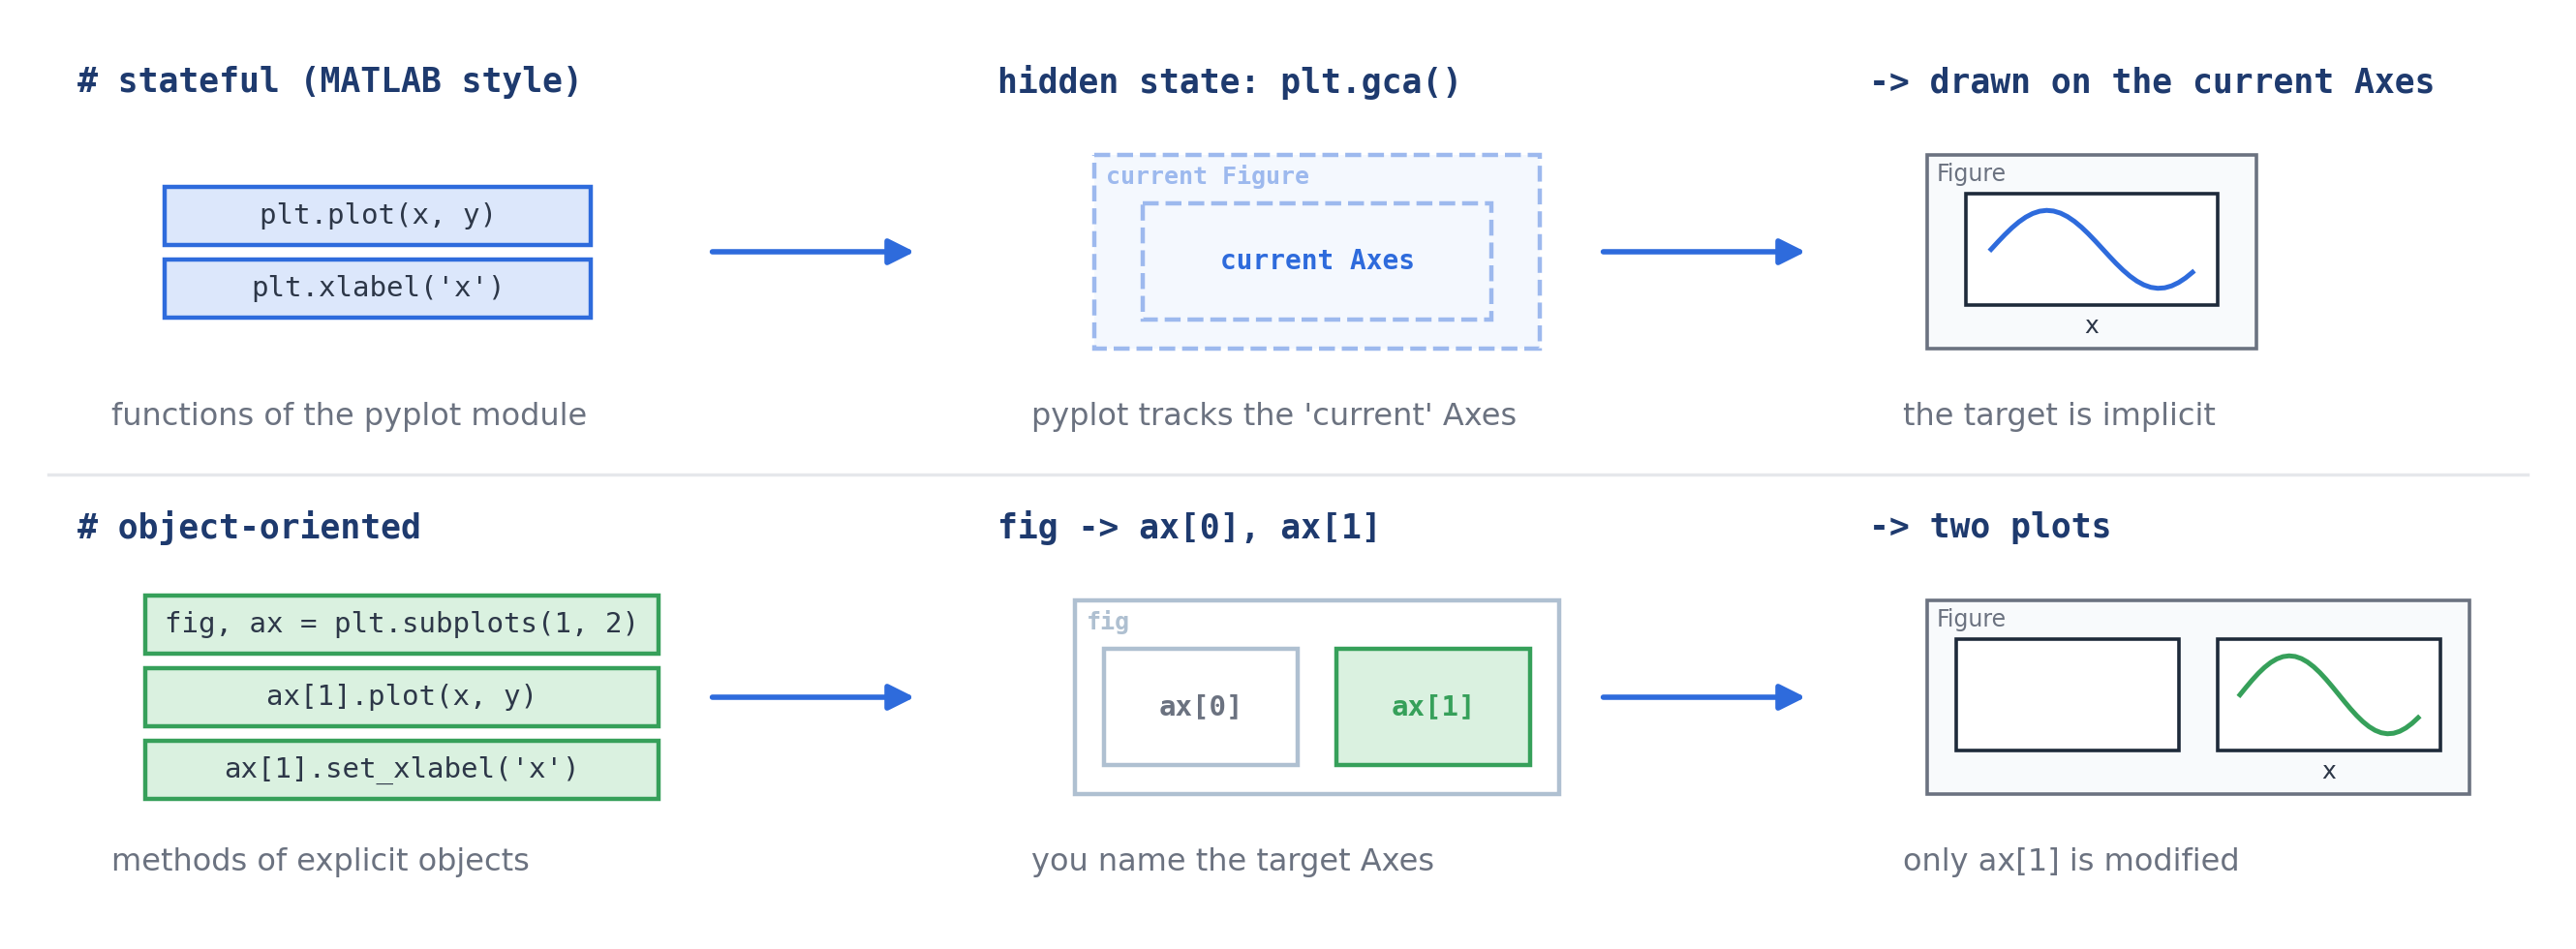
\includegraphics[width=1\textwidth]{contents/images/matplotlib/sub_interfaces.png}
    \caption{The two Matplotlib interfaces: \texttt{pyplot} functions act on the current Axes, tracked implicitly by Matplotlib, while the object-oriented style calls methods on explicit \texttt{Figure} and \texttt{Axes} objects, so the target of each call is always clear.}
\end{figure}

\begin{itemize}
    \item \textbf{Stateful (MATLAB style):} You call functions directly from the \texttt{pyplot} module (e.g., \texttt{plt.plot()}, \texttt{plt.xlabel()}). These functions automatically apply changes to the \textit{current} active Figure and Axes, which Matplotlib tracks in the background.
    \item \textbf{Stateless (Object-Oriented):} You explicitly call methods on specific \texttt{Figure} and \texttt{Axes} objects (e.g., \texttt{ax.plot()}, \texttt{ax.set\_xlabel()}). This approach is strongly recommended because it makes it perfectly clear which plot you are modifying, especially when working with multiple plots at once.
\end{itemize}

\lstinputlisting[caption={Stateful vs. Stateless (Object-Oriented) approaches in Matplotlib.}]{contents/listings/matplotlib/interfaces.py}



\section{Stateless: Figures and Axes}
A \textbf{Figure} is the overall window or image, whereas the \textbf{Axes} are the individual plots contained inside the Figure, each with its own x-axis and y-axis. A single Figure can hold multiple Axes.

\subsection{Creating a Figure and Line Plot}
\begin{itemize}
    \item \texttt{plt.subplots(figsize=(width, height))} creates and returns a new Figure and its associated Axes. The dimensions are specified in inches.
    \item \texttt{ax.plot(x, y)} takes two lists or NumPy arrays containing coordinates and joins the points with line segments. Calling it multiple times on the same Axes automatically adds new lines in different colors.
    \item You can configure the plot's appearance using \texttt{ax.set\_...} methods (e.g., \texttt{ax.set\_xlabel}, \texttt{ax.set\_xlim}, \texttt{ax.set\_xticks}) and add a grid with \texttt{ax.grid()}.
\end{itemize}

\begin{figure}[h]
    \centering
    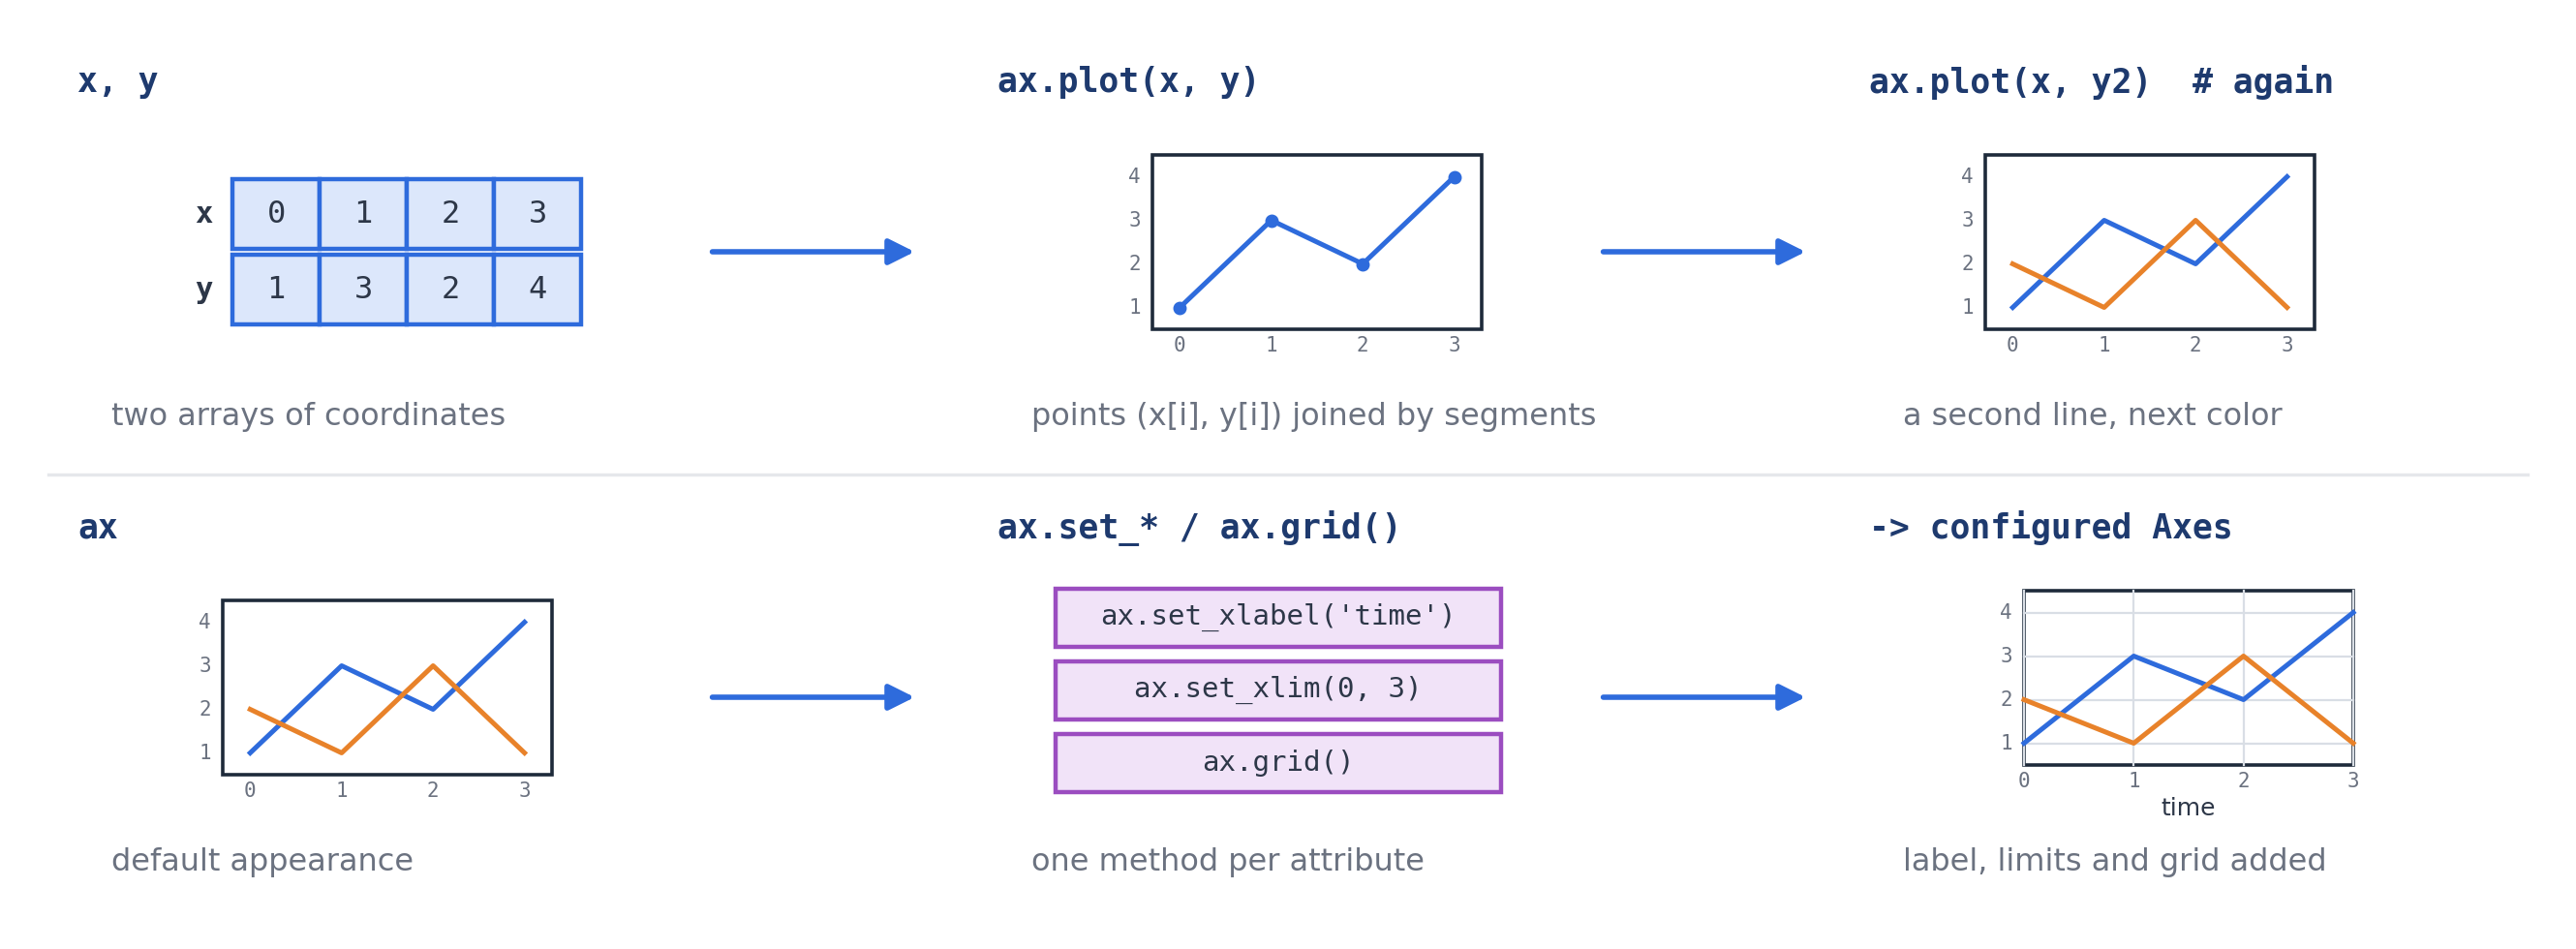
\includegraphics[width=1\textwidth]{contents/images/matplotlib/sub_line_plot.png}
    \caption{Line plots: \texttt{ax.plot(x, y)} joins the points \texttt{(x[i], y[i])} with segments, and each new call adds a line in the next color. The \texttt{ax.set\_...} methods and \texttt{ax.grid()} change one attribute of the Axes at a time.}
\end{figure}

\lstinputlisting[caption={Creating a plot and setting axis attributes using the stateless interface.}]{contents/listings/matplotlib/attributes.py}

\subsection{Creating Many Subplots}
You can create a grid of plots by passing the number of rows and columns as the first two arguments to \texttt{plt.subplots()}.
\begin{itemize}
    \item \textbf{1D Grid:} If you create one row of $n$ Axes, the returned \texttt{ax} object is a 1-D NumPy array of shape \texttt{(n,)}. You access the second plot using \texttt{ax[1]}.
    \item \textbf{2D Grid:} If you create a grid of $m$ rows and $n$ columns, \texttt{ax} is a 2-D array of shape \texttt{(m, n)}. You access the bottom-right plot using coordinate indexing, like \texttt{ax[1, 1]}.
    \item \textbf{Tight Layout:} Always call \texttt{fig.tight\_layout()} at the end of your plotting code to automatically adjust spacing and prevent the labels of neighboring subplots from overlapping.
\end{itemize}

\begin{figure}[h]
    \centering
    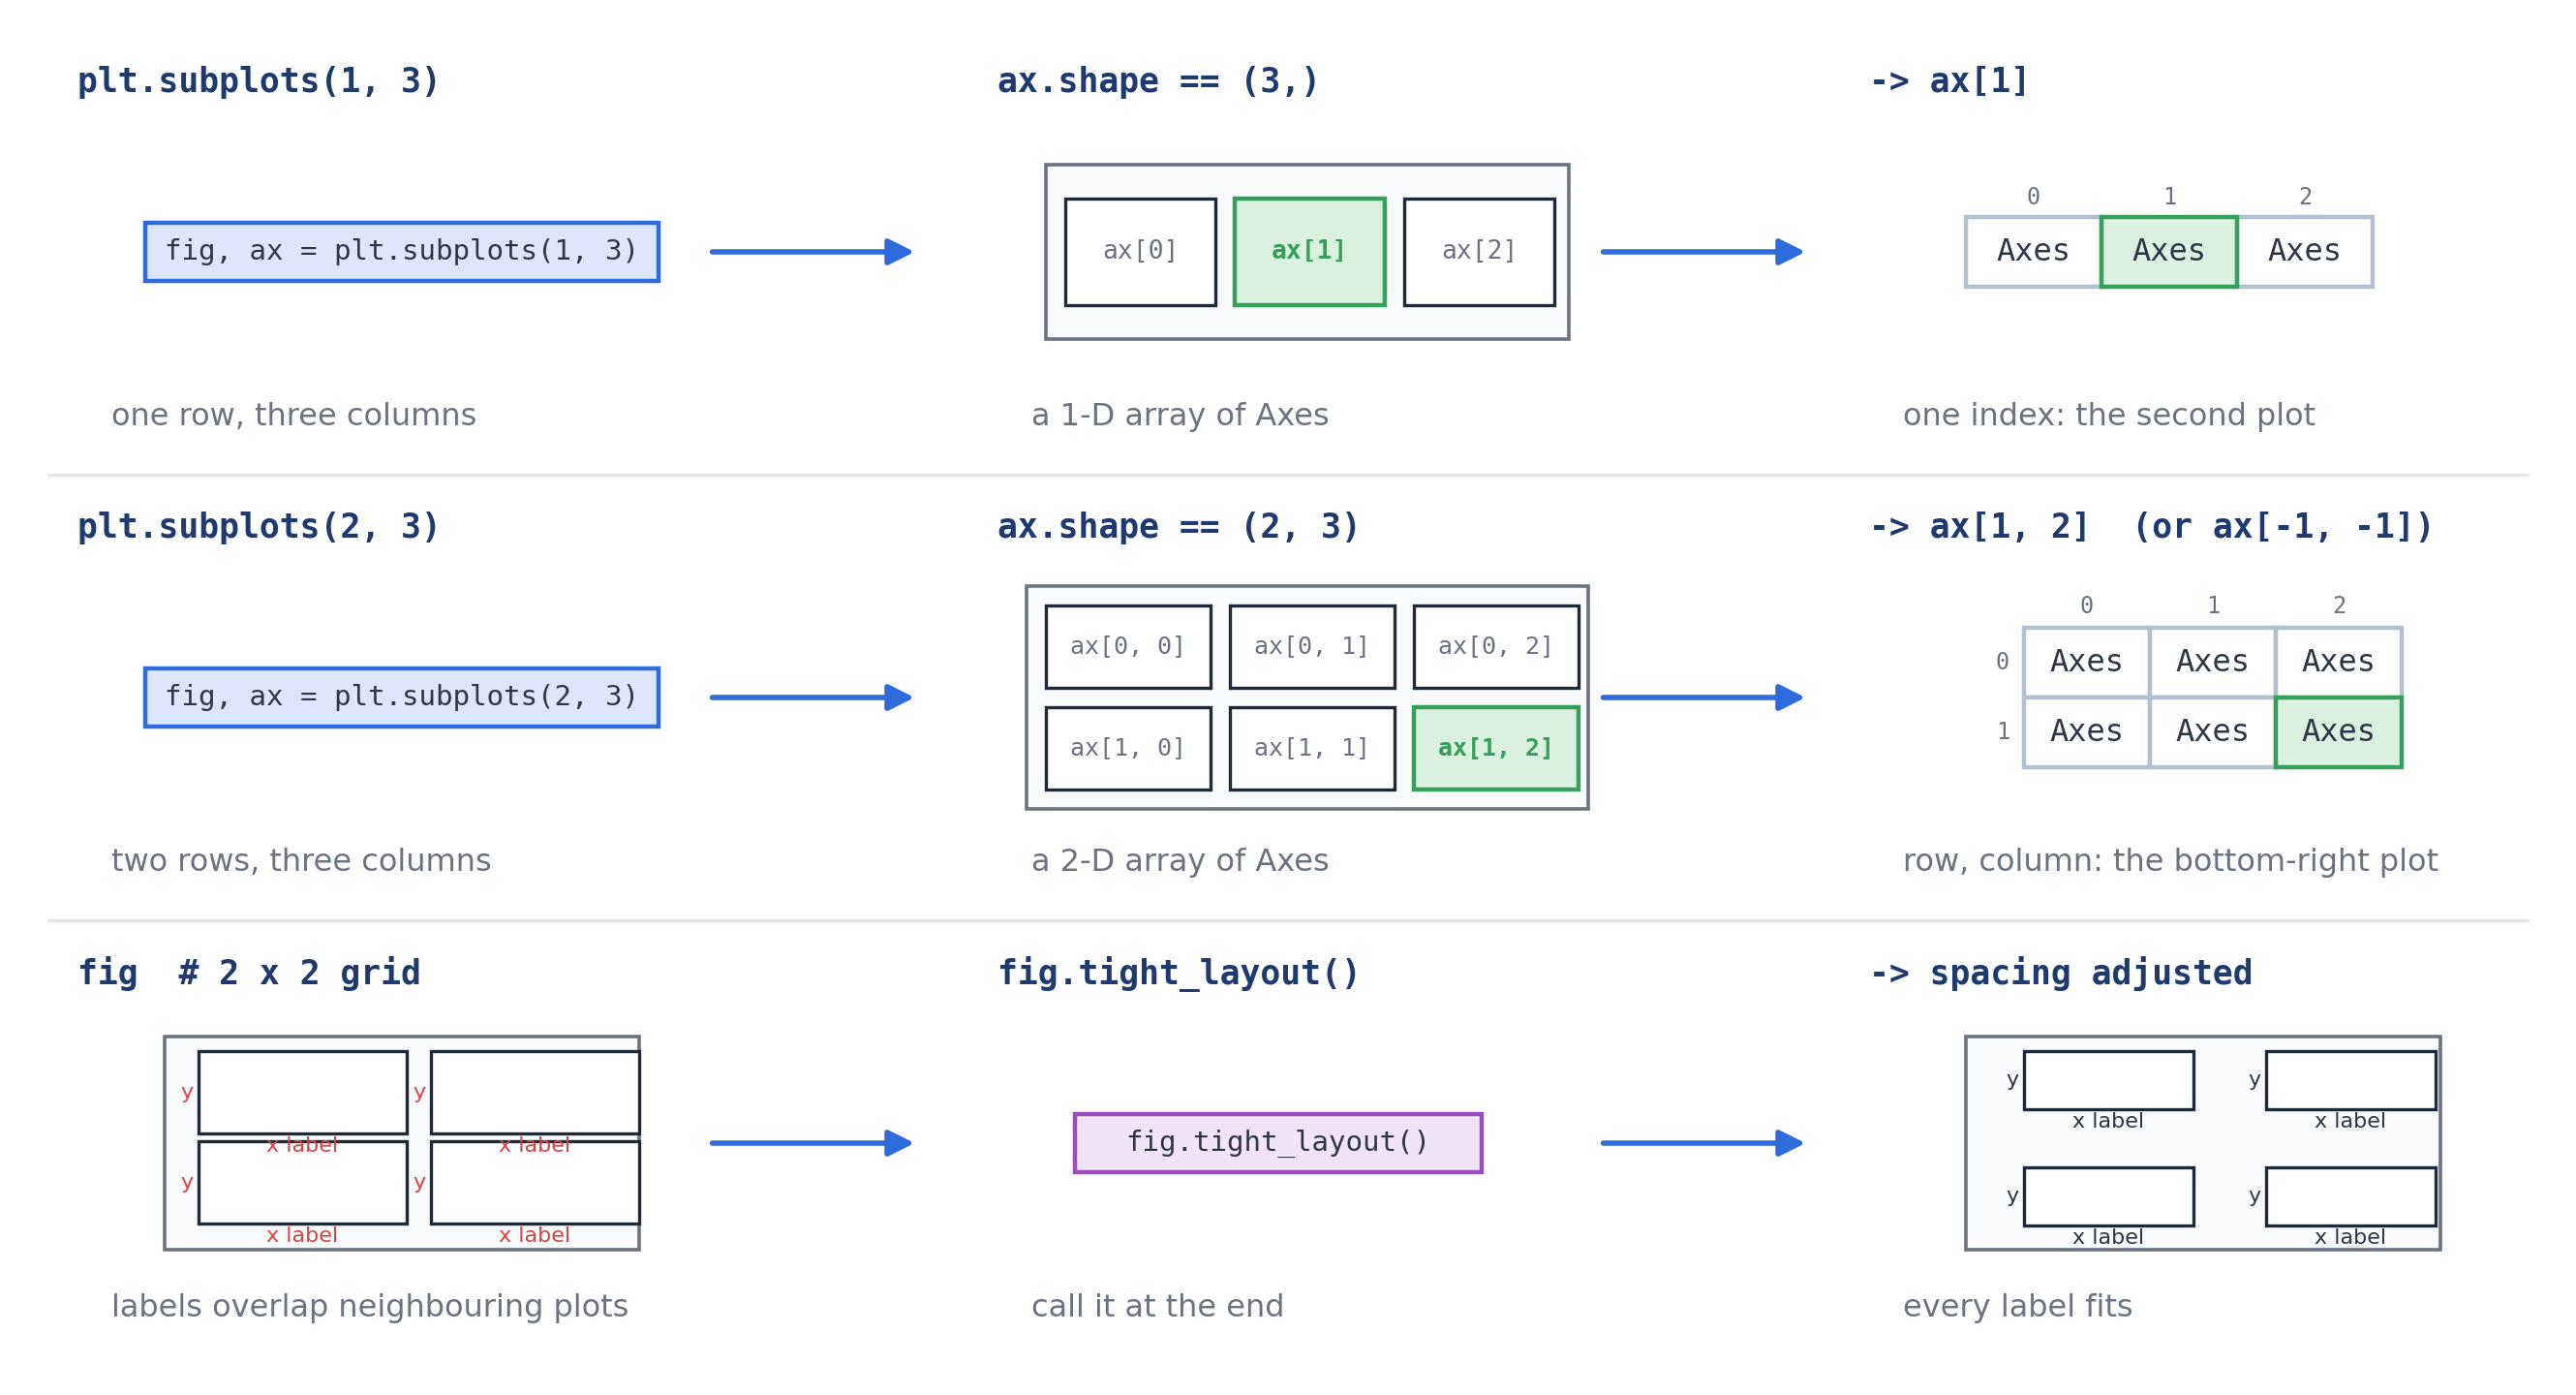
\includegraphics[width=1\textwidth]{contents/images/matplotlib/sub_subplots.png}
    \caption{Subplots: with one row, \texttt{ax} is a 1-D array indexed as \texttt{ax[j]}; with several rows and columns it is a 2-D array indexed as \texttt{ax[i, j]}. \texttt{fig.tight\_layout()} adjusts the spacing so that labels do not overlap.}
\end{figure}

\lstinputlisting[caption={Creating and managing 1D and 2D grids of subplots.}]{contents/listings/matplotlib/subplots.py}



\section{Plot Types}
Matplotlib provides various methods to visualize data. All of these methods are called directly on the \texttt{Axes} object (\texttt{ax}).

\subsection{Line and Scatter Plots}
\begin{itemize}
    \item \textbf{Line Plot (\texttt{ax.plot}):} Draws a sequence of points joined by segments, making it ideal for functions or time series[cite: 163, 171]. You can customize it using keyword arguments like \texttt{linestyle} (\texttt{'-'}, \texttt{'--'}, \texttt{':'}), \texttt{marker} (\texttt{'o'}, \texttt{'*'}), \texttt{color} (or \texttt{c}), and \texttt{label} (used to generate a legend).
    \item \textbf{Scatter Plot (\texttt{ax.scatter}):} Draws a cloud of independent points, useful for showing the relationship between two features. Unlike line plots, you can assign an individual color (\texttt{c}) and size/area (\texttt{s}) to every single point. Colors are usually mapped to numerical values using a colormap (\texttt{cmap}).
\end{itemize}

\begin{figure}[h]
    \centering
    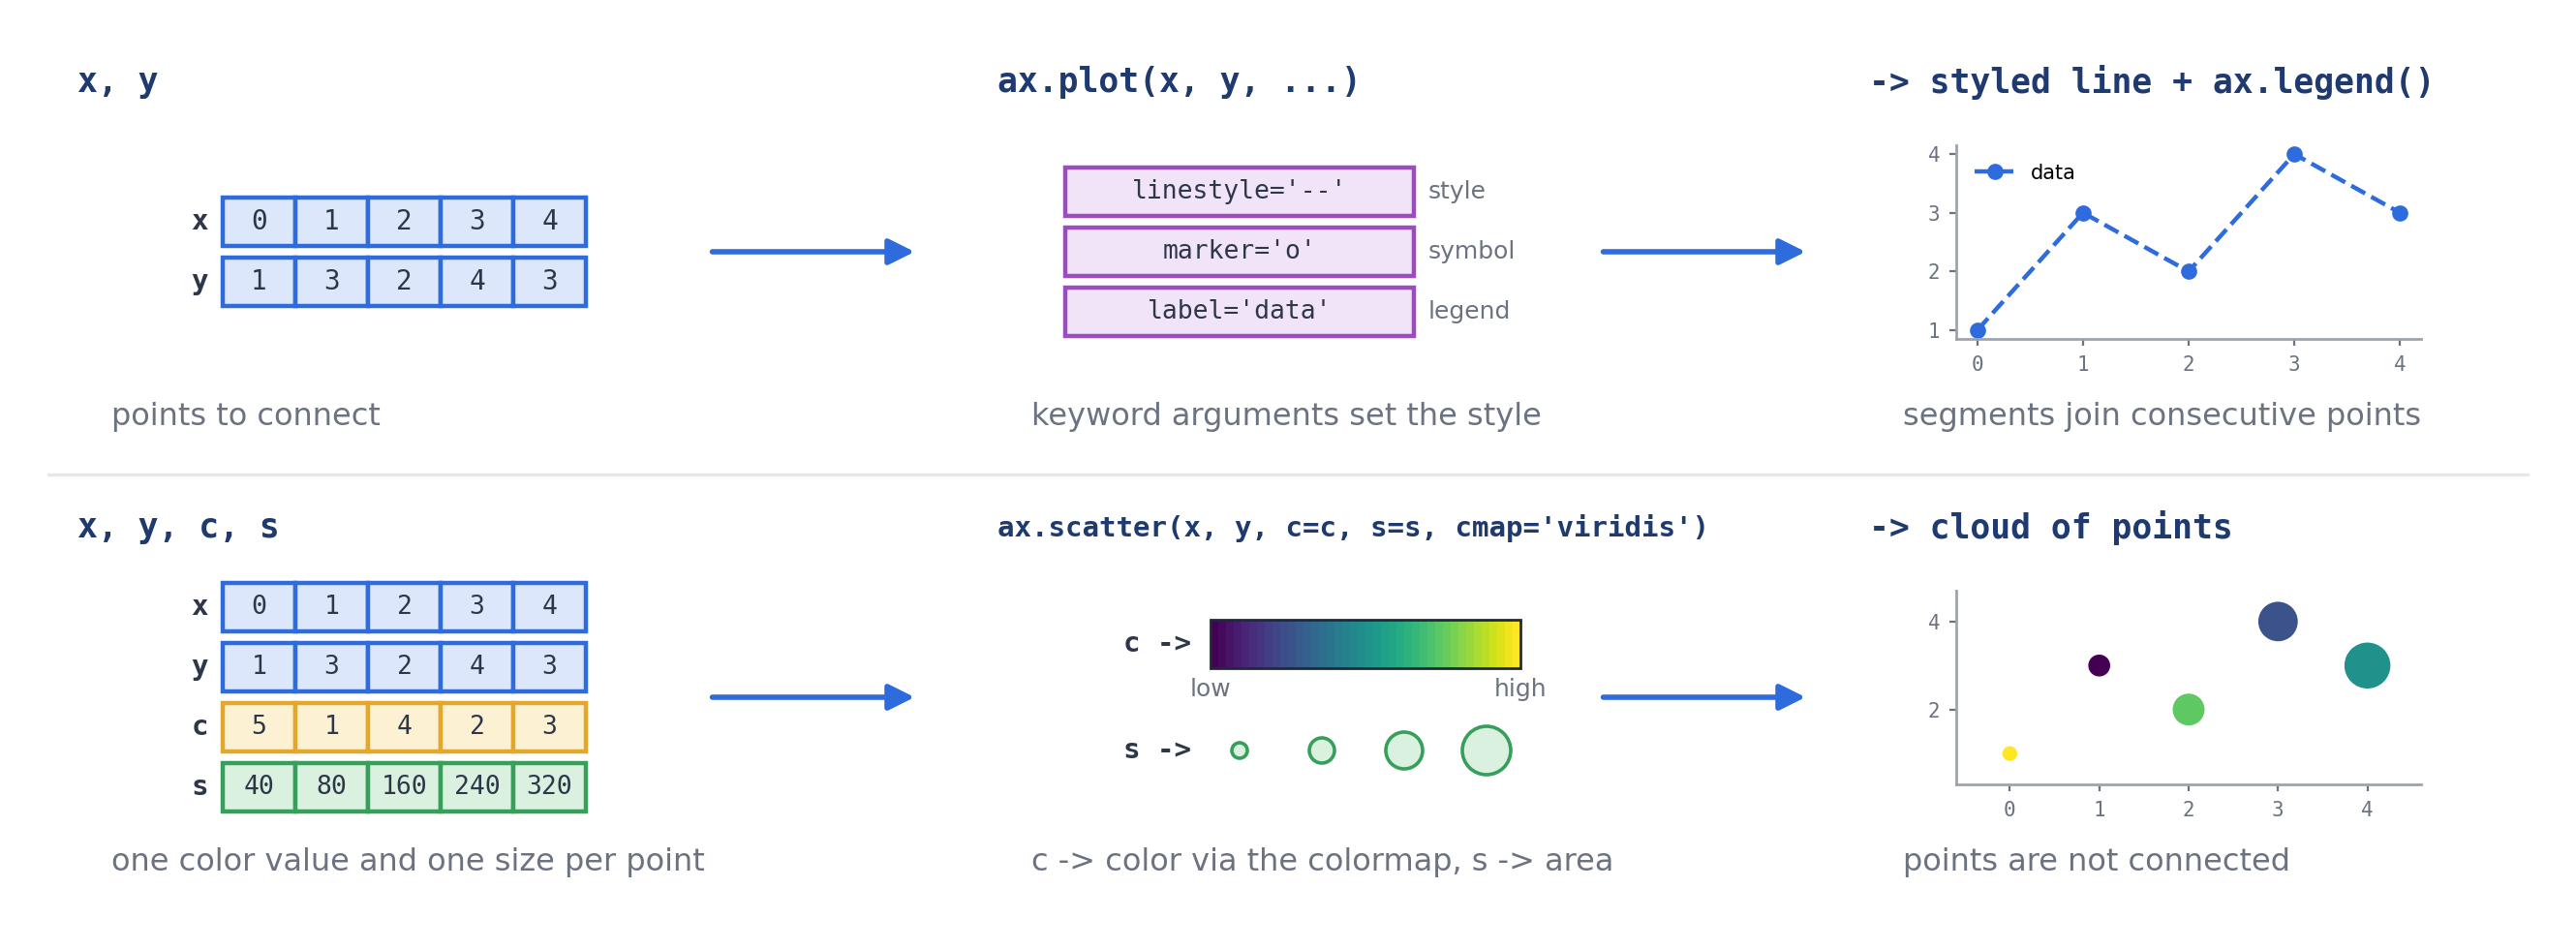
\includegraphics[width=1\textwidth]{contents/images/matplotlib/sub_line_scatter.png}
    \caption{Line and scatter plots: \texttt{ax.plot} joins consecutive points and is styled with keyword arguments such as \texttt{linestyle}, \texttt{marker} and \texttt{label}. \texttt{ax.scatter} draws unconnected points, each with its own color (\texttt{c}, mapped through \texttt{cmap}) and area (\texttt{s}).}
\end{figure}

\lstinputlisting[caption={Creating line plots and scatter plots with varying colors and sizes.}]{contents/listings/matplotlib/line_scatter.py}

\subsection{Bar Charts}
\begin{itemize}
    \item \textbf{Bar Chart (\texttt{ax.bar}):} Displays one numerical value per category. 
    \item To group multiple series of bars side-by-side, you can manually shift their positions along the x-axis (e.g., by subtracting or adding half the bar \texttt{width}) and update the ticks to show the category names.
\end{itemize}

\begin{figure}[h]
    \centering
    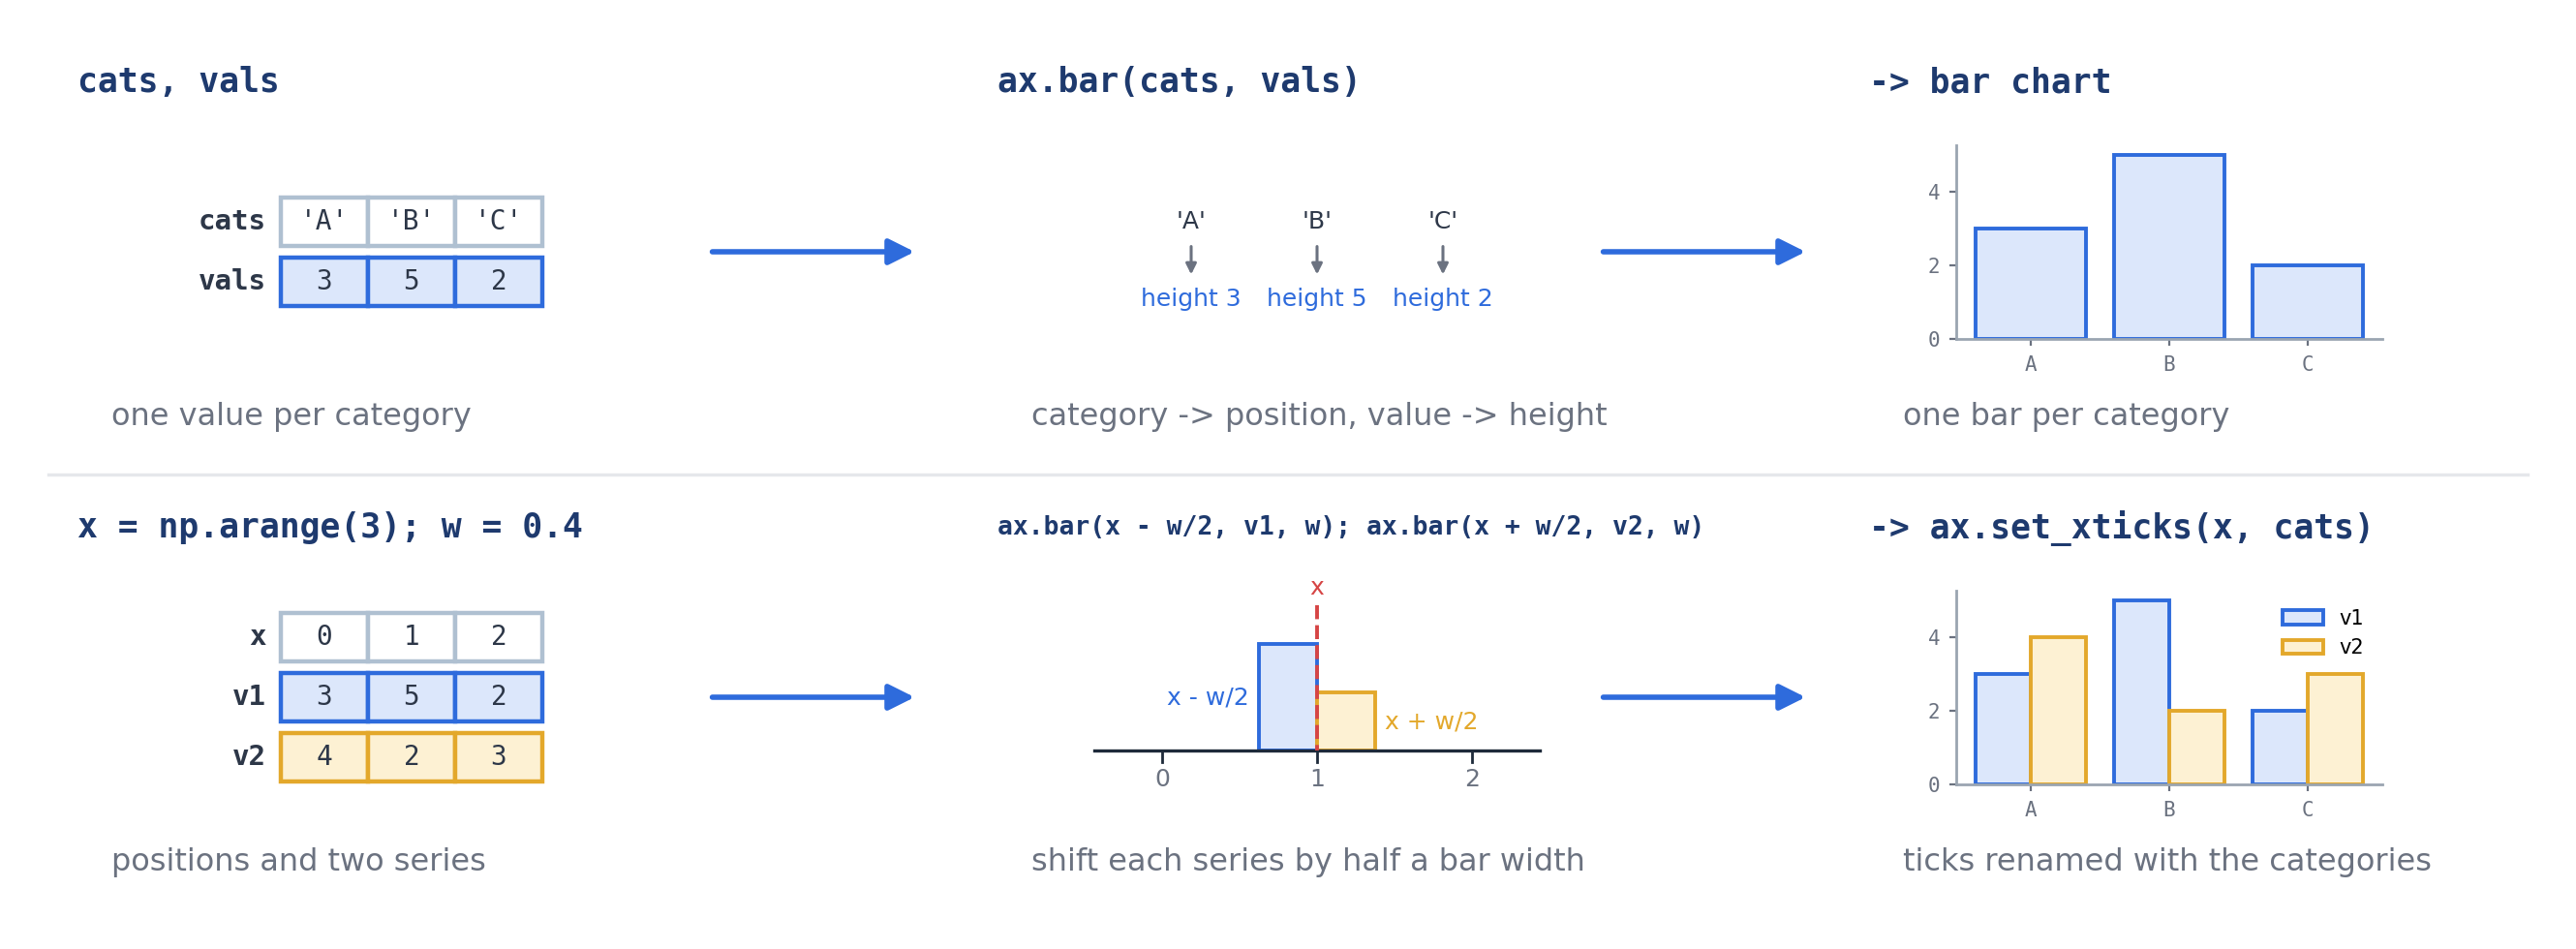
\includegraphics[width=1\textwidth]{contents/images/matplotlib/sub_bar.png}
    \caption{Bar charts: \texttt{ax.bar} draws one bar per category. To group two series, each is shifted by half a bar width around the integer positions \texttt{x}, and \texttt{ax.set\_xticks(x, cats)} puts the category names back on the axis.}
\end{figure}

\lstinputlisting[caption={Creating grouped bar charts.}]{contents/listings/matplotlib/bar.py}

\subsection{Histograms and Text Annotations}

\begin{figure}[h]
    \centering
    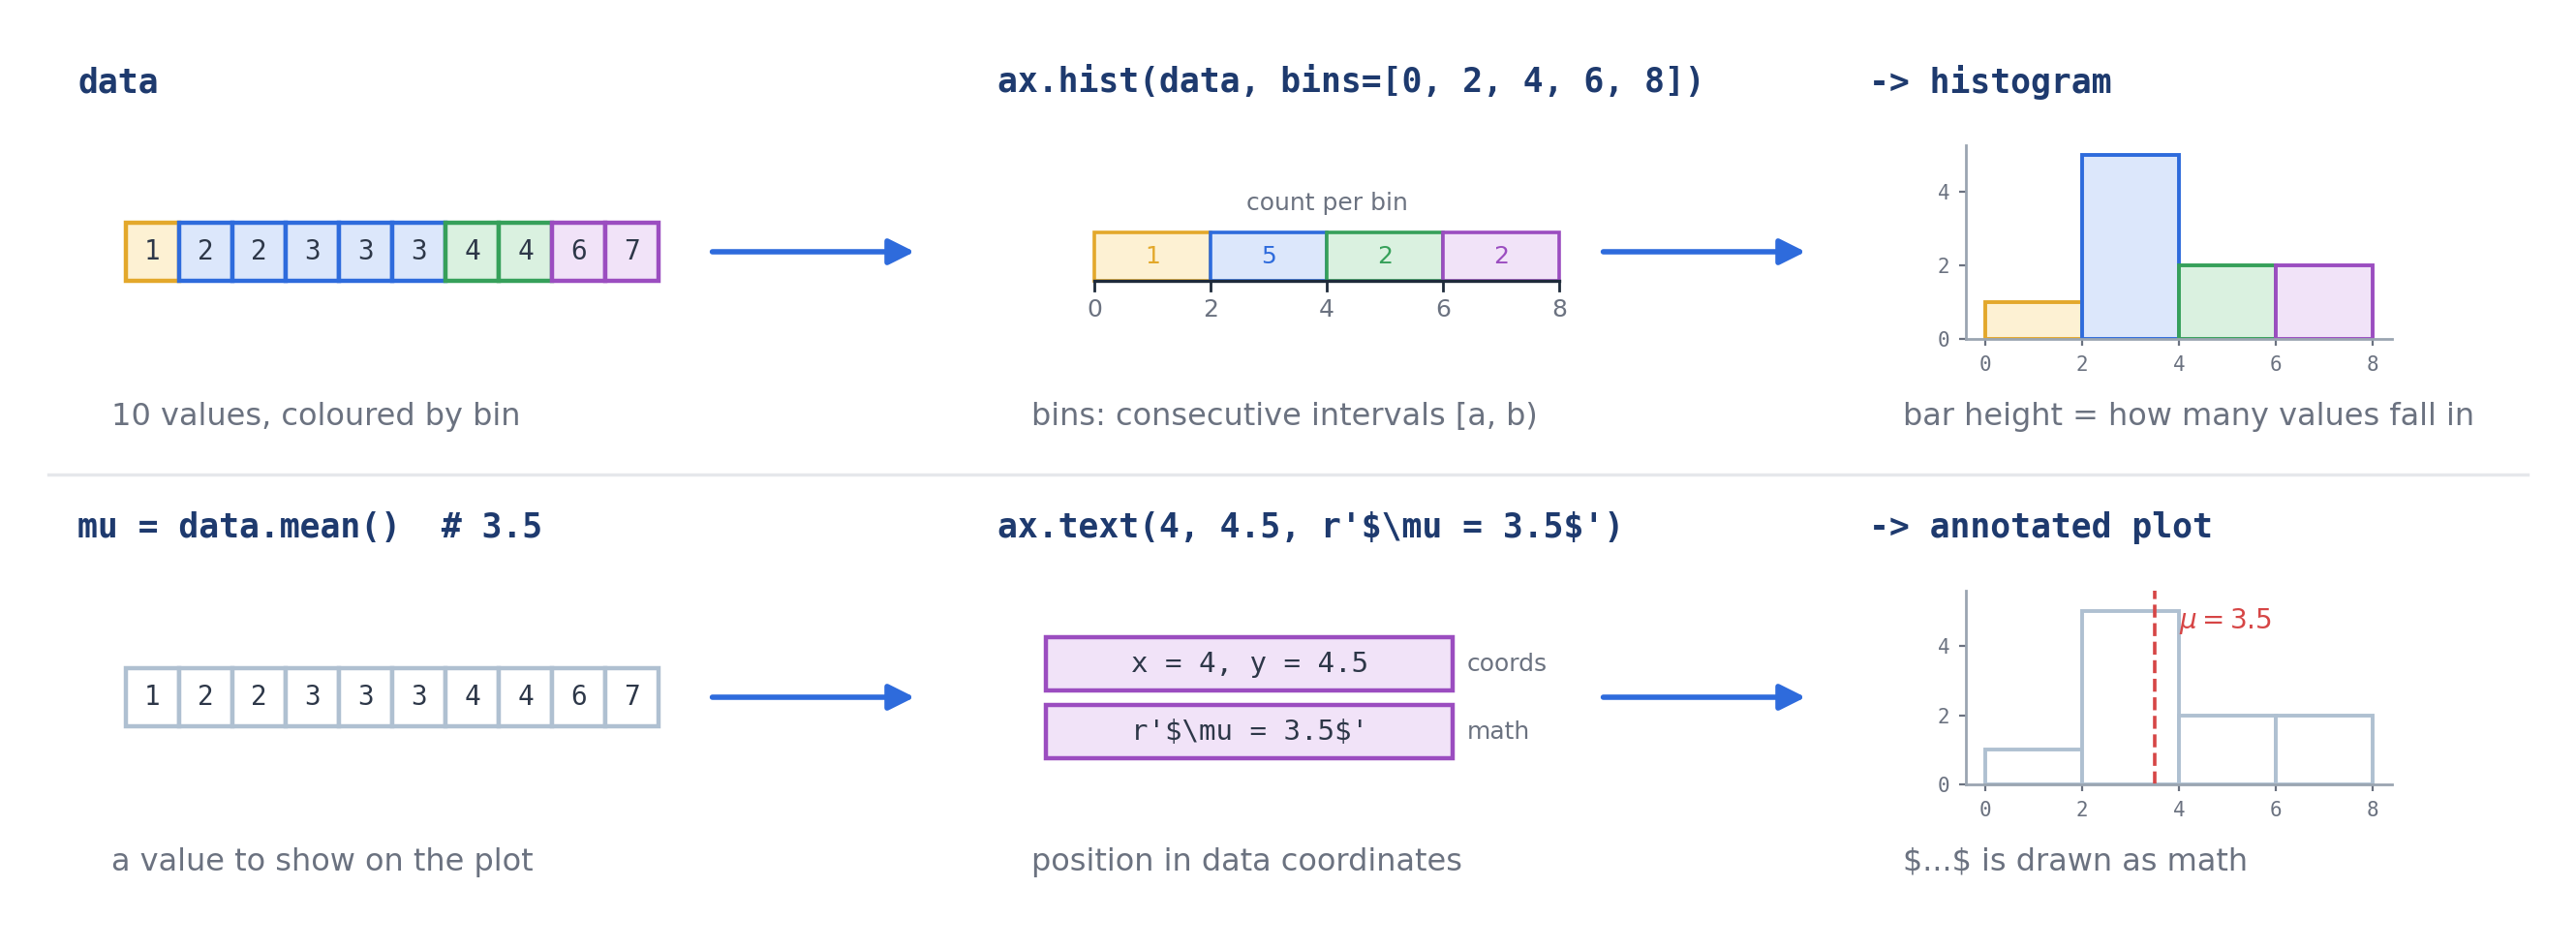
\includegraphics[width=0.85\textwidth]{contents/images/matplotlib/sub_hist_text.png}
    \caption{Histograms and annotations: \texttt{ax.hist} counts how many values fall into each bin (here with explicit edges), and \texttt{ax.text} writes a string at a position given in data coordinates, rendering the part between dollar signs as math.}
\end{figure}

\begin{itemize}
    \item \textbf{Histogram (\texttt{ax.hist}):} Shows the frequency distribution of a single variable, counting how many values fall into consecutive intervals (bins). The \texttt{bins} parameter can be an integer (to specify the number of equal bins) or a NumPy array defining the exact bin edges.
    \item \textbf{Annotations (\texttt{ax.text}):} You can write text directly on the plot by passing data coordinates (\texttt{x}, \texttt{y}). Matplotlib can render LaTeX math equations if the string is enclosed in dollar signs (e.g., \verb|$\mu$|).
\end{itemize}

\subsection{Box Plots}
\begin{itemize}
    \item \textbf{Box Plot (\texttt{ax.boxplot}):} Used to summarize and compare several distributions side-by-side.
    \item The central box extends from the first quartile (Q1) to the third quartile (Q3), with a line marking the median. 
    \item "Whiskers" extend outward to the farthest data points that fall within 1.5 times the Inter-Quartile Range (IQR). Any points beyond the whiskers are plotted as individual markers and are considered candidate outliers (fliers).
\end{itemize}

\begin{figure}[h]
    \centering
    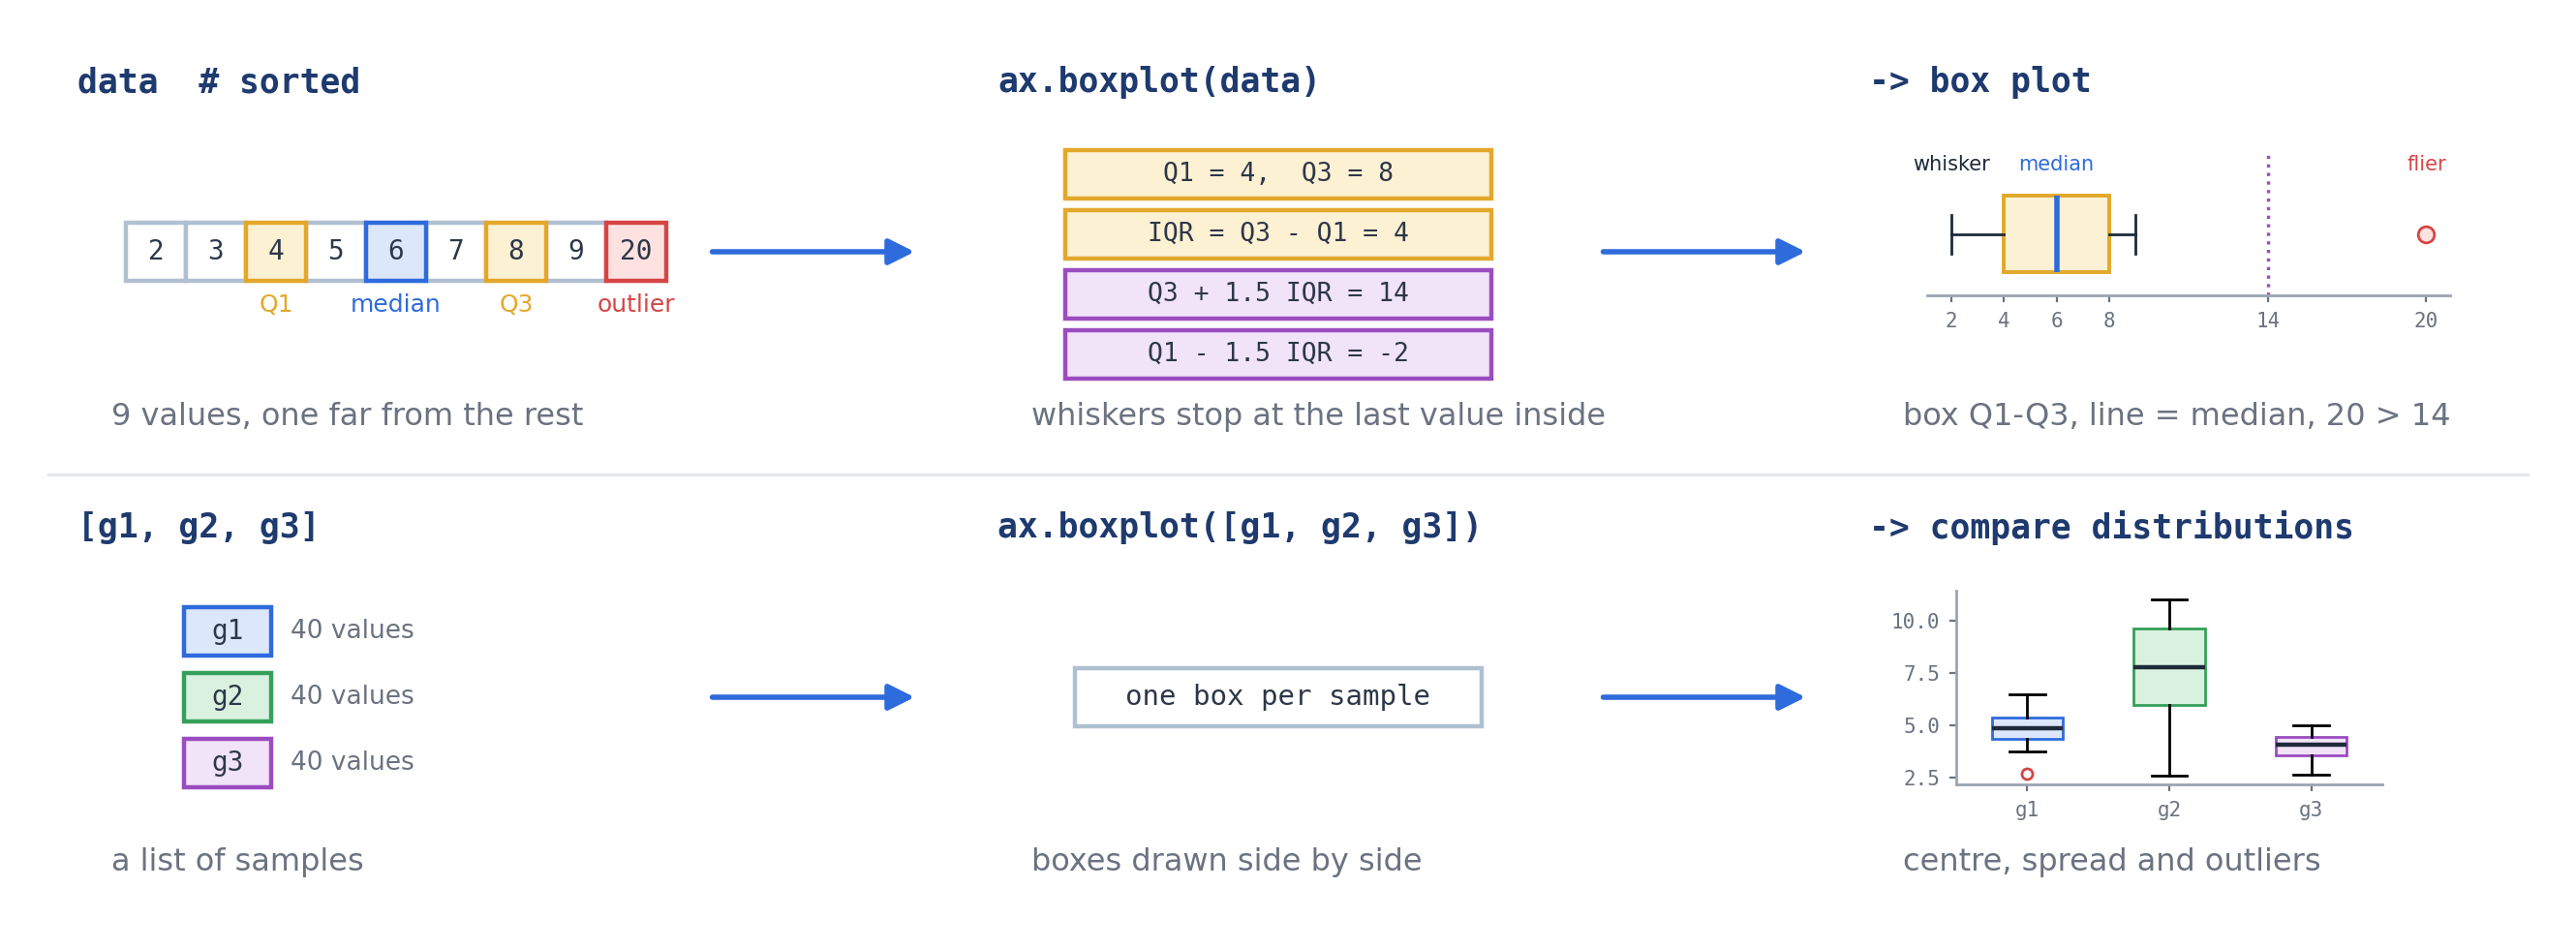
\includegraphics[width=1\textwidth]{contents/images/matplotlib/sub_boxplot.png}
    \caption{Box plots: the box spans Q1 to Q3 with a line at the median; the whiskers reach the farthest values within $1.5\,\mathrm{IQR}$ of the box, and values beyond are drawn as fliers. Passing a list of samples draws one box per sample for comparison.}
\end{figure}

\lstinputlisting[caption={Plotting histograms with text annotations and box plots.}]{contents/listings/matplotlib/hist_box.py}

\subsection{pandas Plotting Integration and Saving}

\begin{figure}[h]
    \centering
    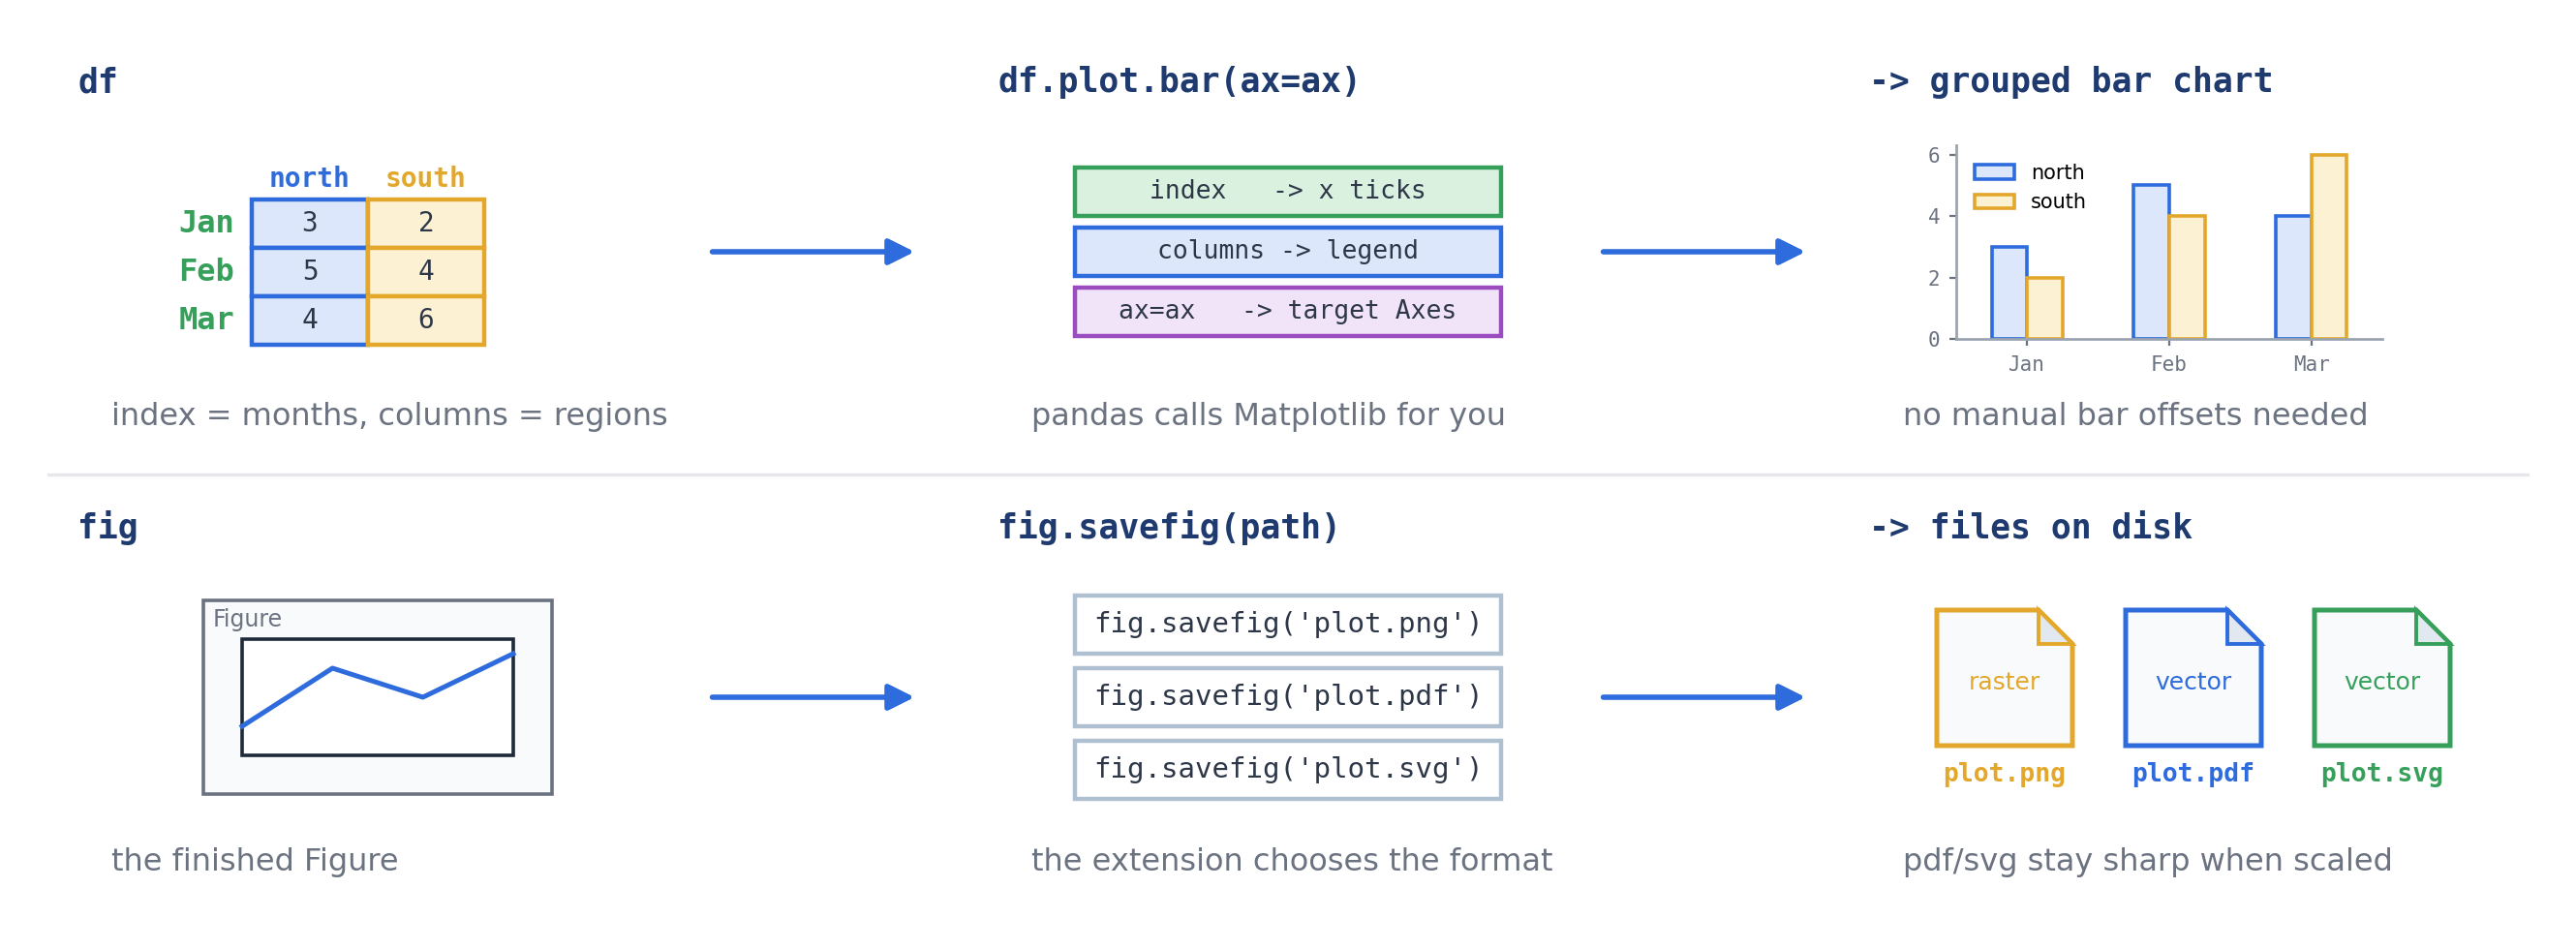
\includegraphics[width=1\textwidth]{contents/images/matplotlib/sub_pandas_plot.png}
    \caption{pandas plotting and saving: \texttt{df.plot.bar(ax=ax)} uses the index for the x-axis ticks and the column names for the legend, drawing on the given Axes. \texttt{fig.savefig} chooses the file format from the extension: PNG is a raster format, PDF and SVG are vector formats.}
\end{figure}

pandas Series and DataFrames have a built-in \texttt{.plot} accessor (e.g., \texttt{df.plot.bar()}) that automatically generates Matplotlib charts. It conveniently uses the DataFrame's index for the x-axis and its column names for the legend. By passing an \texttt{ax} argument (\texttt{ax=ax}), you can direct pandas to draw on your specific stateless Axes.

To save your final figure to disk, use \texttt{fig.savefig(path)}. Matplotlib automatically determines the file format based on the extension you provide (\texttt{.png}, \texttt{.pdf}, \texttt{.svg}, \texttt{.jpg}).







\end{document}
% -----------------------------------------------------------------
